%% This work is released under the LaTeX Project Public License, v1.3c or later.
% This template is made by Ethan Lu.
% Please use XeLaTeX engine!
\documentclass[lang=cn,zihao=-4,a4paper,fontset=windows]{beautybook}
% ---------------------------------------------------------------------------- %
%                            The Cover Theme Chosen                            %
% ---------------------------------------------------------------------------- %
\definecolor{coverbgcolor}{HTML}{e0e0e0}
\definecolor{coverfgcolor}{HTML}{1f3134} % The color of the background
\definecolor{coverbar}{HTML}{7c9092} % The color of the left bar
\definecolor{bottomcolor}{HTML}{2c4f54}
\definecolor{nuanbai}{HTML}{f5f5f5}
\coverstyle={ % 封面键值列表
    cover-choose=cn, % cn ; en ; enfig ; birkar
}
% ---------------------------------------------------------------------------- %
%                            The Cover Theme Chosen                            %
% ---------------------------------------------------------------------------- %
\mathstyle={ % 数学字体键值列表
    math-font=plain, %plain (默认数学字体); stix;  mtpro2
}
\RequirePackage{fontspec}
\setlist{nosep}
\usepackage{subcaption}
\setmainfont{XITS}
\setsansfont{DejaVu Sans}
\setmonofont{Latin Modern Mono}
\renewcommand{\partial}{∂}
%% First one
\mynewtheorem{
    defi={\textbf{Definition}}[section]{interior style={left color=ReD!8,right color=ReD!5!CyaN!50}, borderline west={1.5mm}{0mm}{ReD}},
    thm={\textbf{Theorem}}[section]{interior style={left color=CyaN!80!black!20,right color=CyaN!80!black!15!CyaN!50}, borderline west={1.5mm}{0mm}{CyaN!80!black}},
    lem={\textbf{Lemma}}[section]{interior style={left color=BluE!8,right color=BluE!5!CyaN!50}, borderline west={1.5mm}{0mm}{BluE}},
    prop={\textbf{Proposition}}[section]{interior style={left color=OrangE!8,right color=OrangE!5!CyaN!50}, borderline west={1.5mm}{0mm}{OrangE}},
    exam={\textbf{Example}}[chapter]{interior style={left color=DarkGreen!8,right color=DarkGreen!5!CyaN!50}, borderline west={1.5mm}{0mm}{DarkGreen}},
    cor={\textbf{Corollary}}[chapter]{interior style={left color=violet!8,right color=violet!5!CyaN!50}, borderline west={1.5mm}{0mm}{violet}},
}
\newtheorem*{remark}{\textbf{Remark}}
%% Second one
\makeatletter
\mynewtcbtheorem{
    % 这个 theorem 是环境名
    problem={
        counter=tcbprob, 
        the counter=\thesection.\arabic{tcbprob}, 
        name=Problem, % 它保存到 \theorem@name 里
        thmcolor=绛紫,
        autoref name=\bfseries Problem, 
        style={
        arc=3pt,breakable,enhanced,interior style={top color=绛紫!9 ,middle color=绛紫!6, bottom color=绛紫!3},boxrule=0pt,top=8mm,
        fuzzy shadow={-0.6mm}{0.6mm}{0mm}{0.3mm}{white!50!gray},% 上
        fuzzy shadow={0.6mm}{-0.6mm}{0mm}{0.3mm}{fill=white!40!gray},%下
        opacityframe=0, opacityback=0.98,
        fontupper=\itshape, step={tcbprob},
        before pre=\smallskip, after app=\smallskip,
        overlay unbroken=\my@theorem@overlay@unbroken{Problem\ \thetcbprob}{绛紫},
        overlay first=\my@theorem@overlay@first{Problem\ \thetcbprob}{绛紫},
        overlay last=\my@theorem@overlay@last{绛紫},
        }
    },
    lemma={
        counter=tcblem,
        the counter=\thesection.\arabic{tcblem},
        name=Lemma, 
        lemcolor=靛蓝, 
        autoref name=\bfseries Lemma,
        style={
        arc=0mm,breakable,enhanced,interior style={top color=靛蓝!9 ,middle color=靛蓝!6, bottom color=靛蓝!3},arc=3pt,boxrule=0pt,top=6mm,bottom=5mm,
        fuzzy shadow={-0.6mm}{0.6mm}{0mm}{0.3mm}{white!50!gray},% 上
        fuzzy shadow={0.6mm}{-0.6mm}{0mm}{0.3mm}{fill=white!40!gray},%下
        opacityframe=0, opacityback=0.98,
        fontupper=\itshape,step={tcblem},
        before pre=\smallskip, after app=\smallskip,
        overlay unbroken=\my@lemma@overlay@unbroken{\lemma@name\ \thetcblem}{\lemma@lemcolor},
        overlay first=\my@lemma@overlay@first{\lemma@name\ \thetcblem}{\lemma@lemcolor},
        overlay last=\my@lemma@overlay@last{\lemma@lemcolor},
        }
    },
    corollary={
        counter=tcbcor,
        the counter=\thesection.\arabic{tcbcor},
        autoref name=\bfseries Corollary,
        style={
        arc=0mm,breakable,enhanced,interior style={top color=茶色!9 ,middle color=茶色!6, bottom color=茶色!3},arc=3pt,boxrule=0pt,top=6mm,bottom=5mm,
        fuzzy shadow={-0.6mm}{0.6mm}{0mm}{0.3mm}{white!50!gray},% 上
        fuzzy shadow={0.6mm}{-0.6mm}{0mm}{0.3mm}{fill=white!40!gray},%下
        opacityframe=0, opacityback=0.98,
        fontupper=\itshape,step={tcbcor},
        before pre=\smallskip, after app=\smallskip,
        overlay unbroken=\my@lemma@overlay@unbroken{Corollary\ \thetcbcor}{茶色},
        overlay first=\my@lemma@overlay@first{Corollary\ \thetcbcor}{茶色},
        overlay last=\my@lemma@overlay@last{茶色},
        }
    },
    proposition={
        counter=tcbprop,
        the counter=\thesection.\arabic{tcbprop},
        autoref name=\bfseries Proposition,
        style={
        arc=0mm,breakable,enhanced,interior style={top color=黛绿!9 ,middle color=黛绿!6, bottom color=黛绿!3},arc=3pt,boxrule=0pt,top=6mm,bottom=5mm,
        fuzzy shadow={-0.6mm}{0.6mm}{0mm}{0.3mm}{white!50!gray},% 上
        fuzzy shadow={0.6mm}{-0.6mm}{0mm}{0.3mm}{fill=white!40!gray},%下
        opacityframe=0, opacityback=0.98,
        fontupper=\itshape,step={tcbprop},
        before pre=\smallskip, after app=\smallskip,
        overlay unbroken=\my@lemma@overlay@unbroken{Proposition\ \thetcbprop}{黛绿},
        overlay first=\my@lemma@overlay@first{Proposition\ \thetcbprop}{黛绿},
        overlay last=\my@lemma@overlay@last{黛绿},
        }
    },
    definition={
        counter=tcbdefi,
        the counter=\thesection.\arabic{tcbdefi},
        autoref name=\bfseries Definition,
        style={
        arc=0mm,breakable,enhanced,interior style={top color=茜色!9 ,middle color=茜色!6, bottom color=茜色!3},arc=3pt,boxrule=0pt,top=6mm,bottom=5mm,
        fuzzy shadow={-0.6mm}{0.6mm}{0mm}{0.3mm}{white!50!gray},% 上
        fuzzy shadow={0.6mm}{-0.6mm}{0mm}{0.3mm}{fill=white!40!gray},%下
        opacityframe=0, opacityback=0.98,
        fontupper=\normalsize,step={tcbdefi},
        before pre=\smallskip, after app=\smallskip,
        overlay unbroken=\my@lemma@overlay@unbroken{Definition\ \thetcbdefi}{茜色},
        overlay first=\my@lemma@overlay@first{Definition\ \thetcbdefi}{茜色},
        overlay last=\my@lemma@overlay@last{茜色},
        }
    },
    example={
        counter=tcbexam,
        the counter=\thesection.\arabic{tcbexam},
        autoref name=\bfseries Example,
        style={
        arc=0mm,breakable,enhanced,interior style={top color=黛绿!9 ,middle color=黛绿!6, bottom color=黛绿!3},arc=3pt,boxrule=0pt,top=6mm,bottom=5mm,
        fuzzy shadow={-0.6mm}{0.6mm}{0mm}{0.3mm}{white!50!gray},% 上
        fuzzy shadow={0.6mm}{-0.6mm}{0mm}{0.3mm}{fill=white!40!gray},%下
        opacityframe=0, opacityback=0.98,
        fontupper=\normalsize,step={tcbexam},
        before pre=\smallskip, after app=\smallskip,
        overlay unbroken=\my@lemma@overlay@unbroken{Example\ \thetcbexam}{黛绿},
        overlay first=\my@lemma@overlay@first{Example\ \thetcbexam}{黛绿},
        overlay last=\my@lemma@overlay@last{黛绿},
        }
    },
    Exercise={
        counter=tcbexer,
        the counter=\thechapter.\arabic{tcbexer},
        autoref name=\bfseries Exercise,
        style={
        arc=0mm,breakable,enhanced,interior style={top color=绛紫!9 ,middle color=绛紫!6, bottom color=绛紫!3},arc=3pt,boxrule=0pt,top=6mm,bottom=5mm,
        fuzzy shadow={-0.6mm}{0.6mm}{0mm}{0.3mm}{white!50!gray},% 上
        fuzzy shadow={0.6mm}{-0.6mm}{0mm}{0.3mm}{fill=white!40!gray},%下
        opacityframe=0, opacityback=0.9,
        fontupper=\normalsize,step={tcbexer},
        before pre=\smallskip, after app=\smallskip,
        overlay unbroken=\my@lemma@overlay@unbroken{Exercise\ \thetcbexer}{绛紫},
        overlay first=\my@lemma@overlay@first{Exercise\ \thetcbexer}{绛紫},
        overlay last=\my@lemma@overlay@last{绛紫},
        }
    },
    theorem={
        counter=tcbthm,
        the counter=\thesection.\arabic{tcbthm},
        autoref name=\bfseries Theorem,
        style={
        arc=0mm,breakable,enhanced,interior style={top color=黛绿!9 ,middle color=黛绿!6, bottom color=黛绿!3},arc=3pt,boxrule=0pt,top=6mm,bottom=5mm,
        fuzzy shadow={-0.6mm}{0.6mm}{0mm}{0.3mm}{white!50!gray},% 上
        fuzzy shadow={0.6mm}{-0.6mm}{0mm}{0.3mm}{fill=white!40!gray},%下
        opacityframe=0, opacityback=0.98,
        fontupper=\itshape,step={tcbthm},
        before pre=\smallskip, after app=\smallskip,
        overlay unbroken=\my@lemma@overlay@unbroken{Theorem\ \thetcbthm}{黛绿},
        overlay first=\my@lemma@overlay@first{Theorem\ \thetcbthm}{黛绿},
        overlay last=\my@lemma@overlay@last{黛绿},
        }
    },
    conjecture={
        counter=tcbconj,
        the counter=\thesection.\arabic{tcbconj},
        name=Conjecture, 
        lemcolor=靛蓝, 
        autoref name=\bfseries Conjecture,
        style={
        arc=0mm,breakable,enhanced,interior style={top color=靛蓝!9 ,middle color=靛蓝!6, bottom color=靛蓝!3},arc=3pt,boxrule=0pt,top=6mm,bottom=5mm,
        fuzzy shadow={-0.6mm}{0.6mm}{0mm}{0.3mm}{white!50!gray},% 上
        fuzzy shadow={0.6mm}{-0.6mm}{0mm}{0.3mm}{fill=white!40!gray},%下
        opacityframe=0, opacityback=0.98,
        fontupper=\itshape,step={tcbconj},
        before pre=\smallskip, after app=\smallskip,
        overlay unbroken=\my@lemma@overlay@unbroken{Conjecture\ \thetcblem}{靛蓝},
        overlay first=\my@lemma@overlay@first{Conjecture\ \thetcblem}{靛蓝},
        overlay last=\my@lemma@overlay@last{靛蓝},
        }
    },
}
\makeatother

%% --------参考文献
\RequirePackage[
backend=biber,
style=numeric,
sorting=nty
]{biblatex}
\addbibresource{ref.bib}

\indexsetup{level=\chapter*,noclearpage}
\makeindex[title={\sffamily References},columns=3,columnsep=15pt,columnseprule]
\makeindex

    \usepackage{listings}
    \lstset{
        basicstyle=\small\ttfamily,	
            keywordstyle=\color{NavyBlue}, 
            commentstyle=\color{gray!50!black!50},   	
            stringstyle=\rmfamily\slshape\color{red}, 	
        backgroundcolor=\color{gray!5},     
        frame=leftline,						
        framerule=0.5pt,rulecolor=\color{gray!80}, 
        numbers=left,				
            numberstyle=\footnotesize,	
            firstnumber=1,
            stepnumber=1,                  	
            numbersep=7pt,               	
        aboveskip=.25em, 			
        showspaces=false,               	
        showstringspaces=false,        
        keepspaces=true, 					
        showtabs=false,                 	
        tabsize=2,                     		
        captionpos=b,                   	
        flexiblecolumns=true, 			
        breaklines=true,                	
        breakatwhitespace=false,        	
        breakautoindent=true,			
        breakindent=1em, 			
        title=\lstname,				
        escapeinside=``,  		
        xleftmargin=1em,  xrightmargin=1em,     
        aboveskip=1ex, belowskip=1ex,
        framextopmargin=1pt, framexbottommargin=1pt,
            abovecaptionskip=-2pt,belowcaptionskip=3pt,
        extendedchars=false, columns=flexible, mathescape=true,
        texcl=true,
        fontadjust
    }%
% 设置1.25倍行距
\linespread{1.25}
\setlist[itemize]{itemsep=1pt, parsep=1pt} % 对所有itemize环境生效
\setlist[enumerate]{itemsep=1pt, parsep=1pt} % 对所有enumerate环境生效
\begin{document}
\thispagestyle{empty}
\title{ 学习与优化}
\subtitle{学习笔记}
\edition{First Edition}
\bookseries{ }
\author{夏同}
\pressname{Beautybook}
\presslogo{inner_pics/beautybooK-logo.png}
\coverimage{inner_pics/coverimage.jpg}%ivy-ge998908f8_1280.jpg
\makecover

\makeatletter
% ---------------------------------------------------------------------------- %
%                           The Sidebar Theme Chosen                           %
% ---------------------------------------------------------------------------- %
\definecolor{bg}{HTML}{e0e0e0}
\definecolor{fg}{HTML}{2c4f54}
\colorlet{outermarginbgcolor}{bg}
\colorlet{outermarginfgcolor}{fg}
% set the contents of the outer margin on even and odd pages for scrheadings, plain and scth
\oddoutermargin{\sffamily \leftmark} % Odd
\evenoutermargin{\sffamily\@title} % Even
% ---------------------------------------------------------------------------- %
%                           The Sidebar Theme Chosen                           %
% ---------------------------------------------------------------------------- %

% ---------------------------------------------------------------------------- %
%                         The images used in the title                         %
% ---------------------------------------------------------------------------- %
\titleimage{
  chapteroddimage={odd1,odd2,odd3,odd4,odd5,odd6,odd7,odd8,odd9,odd10,odd11,odd12,odd13,odd14,odd15,mid1,mid2,mid3,mid4,mid5,mid6,mid7,mid8,mid9,mid10,mid11},
%
  partoddimage={odd1,odd2,odd3,odd4,odd5,odd6,odd7,odd8,odd9,odd10,odd11,odd12,odd13,odd14,odd15,mid1,mid2,mid3,mid4,mid5,mid6,mid7,mid8,mid9,mid10,mid11},
%
  chapterevenimage={songeven,even1,even2,even3,even4,mid1,mid2,mid3,mid4,mid5,mid6,mid7,mid8,mid9,mid10,mid11},
%
  partevenimage={songeven,even1,even2,even3,even4,mid1,mid2,mid3,mid4,mid5,mid6,mid7,mid8,mid9,mid10,mid11},
}
\chapimage{\beautybook@chapterimagename} % 会自动改变
\partimage{\beautybook@partimagename}    % 会自动改变
\makeatother
% ---------------------------------------------------------------------------- %
%                         The images used in the title                         %
% ---------------------------------------------------------------------------- %

% ---------------------------------------------------------------------------- %
%                      The Color Chosen for The Magic Box                      %
% ---------------------------------------------------------------------------- %
\colorlet{framegolden}{fg} % The line color of the magic box
\colorlet{framegray}{bg!50} % The background color of the magic box
% ---------------------------------------------------------------------------- %
%                      The Color Chosen for The Magic Box                      %
% ---------------------------------------------------------------------------- %

\frontmatter
\pagenumbering{Roman}

{% Preface
% \addcontentsline{toc}{chapter}{Preface}
\chapter*{前言}
本书所讲解的的知识内容来自笔者在B站观看的课程《学习与优化》，讲课老师为华南理工大学龚老师。


\hfill
\begin{tabular}{lr}
    &--- 夏同\\ 
    &\today
\end{tabular}
\clearpage}


\tableofcontents\let\cleardoublepage\clearpage

\mainmatter
\pagenumbering{arabic}

\partabstract{\hspace*{2em} 深度学习，机器学习等知识是该课程的主要内容}
\part{深度学习}

\chapter{神经网络与深度学习基础}

\section{启发性思考}
深度学习的核心思想是模仿人脑处理信息的方式。人脑中约有860亿个神经元，每个神经元通过树突接收信号，在细胞体整合，若超过某个阈值则通过轴突释放信号（电脉冲）至其他神经元。这一“全有或全无”的激发模式启发了最早的数学模型——\textbf{人工神经元}（或称感知器）。

本章将系统学习：
\begin{itemize}
    \item 人工神经元的基本组成：\textbf{权重}、\textbf{偏置}、\textbf{激活函数}
    \item 几种经典激活函数（Sigmoid, tanh, ReLU）的特性与对比
    \item \textbf{前馈神经网络}的结构与矩阵表示
    \item \textbf{Softmax函数}及其温度系数的妙用
    \item 神经网络训练的完整流程：\textbf{前向传播}、\textbf{损失函数}、\textbf{梯度下降}与核心算法——\textbf{反向传播（Backpropagation, BP）}
\end{itemize}


\section{神经元：深度学习的基石}

\subsection{为什么需要神经元？}
人工神经网络的设计灵感源于对生物神经系统的简化模拟。在大脑中，数十亿个神经元通过复杂的连接处理信息：每个神经元接收来自其他神经元的信号，当这些信号的累积超过某个阈值时，该神经元被激活，并向下一级神经元传递自己的信号。模仿这一机制，我们可以构造一个简单的数学单元（人工神经元）作为深度学习模型的基本构件。它的目标是从输入数据中学习出有意义的特征表示，从而完成分类、回归等任务。

\subsection{类比人类神经元}
因此，为了构造人工神经元的数学模型，我们需要思考人类的行为，再进行类比。如果把神经元比作一个人在听取多方意见后做决定，那么权重就类似于你对每个朋友发言的“信任度”或“重视程度”。有些朋友（高权重）的话会极大地影响你的最终决定，而另一些朋友（低权重）则可有可无。权重可以是正的（朋友支持）也可以是负的（朋友反对），甚至为零（忽略）。

从数学上看，权重和输入的关系其实是一个简单的“加权求和”过程：我们把每个输入 $x_i$ 乘以对应的权重 $w_i$，再把所有乘积加起来，最后加上偏置 $b$。写成公式就是 $z = w_1 x_1 + w_2 x_2 + \dots + w_n x_n + b$。这个公式用向量符号可以简洁地表示为 $z = \mathbf{w} \cdot \mathbf{x} + b$，其中 $\mathbf{w} \cdot \mathbf{x}$ 表示两个向量对应分量相乘再相加，即“点积”。点积的几何意义可以理解为：向量 $\mathbf{x}$ 在向量 $\mathbf{w}$ 方向上的投影长度再乘以 $\mathbf{w}$ 的长度。换句话说，权重向量 $\mathbf{w}$ 指定了一个“方向”，而加权和 $z$ 的大小反映了输入 $\mathbf{x}$ 在这个方向上的“分量”。

有人会问，公式$z = \mathbf{w} \cdot \mathbf{x+ b}$中，后面的$\mathbf{b}$是什么呢？观察公式，我们会发现，即使没有任何外部信息（即所有输入 $x_i = 0$），神经元也可能有被激活的倾向，这就是偏置 $b$ 的作用。延续上面的类比，偏置可以看作你与生俱来的性格底色，或者在没有外界意见时的“预设立场”。如果偏置为正，那么即便没有输入信号，神经元也倾向于兴奋；反之，如果偏置为负，则需要较强的外部信号才能将其激活。从几何上讲，偏置使得决策边界不必通过原点，提供了平移的自由度，从而显著增强模型的表达能力。例如在二维平面中，若没有偏置，分类直线必须穿过原点，这显然过于局限；偏置允许我们将直线移动到任何位置。

那么权重和偏置如何决定一个分类决策呢？想象一个二维平面，每个输入点 $(x_1, x_2)$ 要么属于类别A，要么属于类别B。一个神经元可以学会用一条直线来划分这两个类别——这条直线就是所谓的“决策边界”（在高维空间中，它被称为“超平面”，其实就是直线、平面概念的推广）。权重向量 $\mathbf{w}$ 的方向正好垂直于这条直线，决定了直线的倾斜角度；而偏置 $b$ 决定了直线离开原点的距离。改变权重，就相当于旋转这条直线；改变偏置，就相当于平移它。训练神经网络的过程，就是通过不断微调这些权重和偏置，让这条直线（或超平面）能够恰好将不同类别的点分开，使得神经元的输出 $a = f(z)$ 尽可能地接近我们期望的标签（比如类别A输出1，类别B输出0）。这种调整靠的是从大量例子中“学习”：给网络看很多带标签的样本，让它自己摸索出最合适的直线位置。

然而，神经元最终是要组成神经网络的。倘若只有加权和与偏置，那无论堆叠多少层神经元，整个网络仍然等价于一个线性模型（因为线性函数的复合仍是线性的），永远无法模拟现实世界中千变万化的非线性现象。激活函数的引入打破了这一僵局，它给神经元注入了“灵魂”。

\begin{definition}[][神经元的数学模型]
一个典型的人工神经元接收 $n$ 个输入 $x_1, x_2, \ldots, x_n$（例如，一张图片的像素值或一条文本的词向量）。每个输入都对应一个可学习的参数，即“权重” $w_i$，它决定了该输入对神经元输出的重要性。此外，神经元还有一个额外的参数“偏置”$b$，它可以理解为神经元的“固有倾向”。首先，神经元计算输入的加权和（称为“预激活值”）：
\[
z = \sum_{i=1}^{n} w_i x_i + b
\]
再将 $z$ 送入一个非线性函数 $f$（称为“激活函数”），得到神经元的最终输出：
\[
a = f(z)
\]
\end{definition}

上文提到，如果没有非线性，无论神经元堆叠多少层，整个神经网络仍然等价于一个线性模型，无法学习复杂的模式。这是为什么呢？让我们从一个直观例子入手：假设我们想用一条直线将平面上的两类点分开。如果这两类点是线性可分的（比如被一条直线分开），那么一个简单的线性模型就足够了。但现实中的数据往往更复杂，比如经典的“异或”（XOR）问题：两个输入 $(0,0)$ 和 $(1,1)$ 属于一类，$(0,1)$ 和 $(1,0)$ 属于另一类。你无法用任何一条直线将它们分开，必须使用曲线或折线。线性模型（无论多少层线性变换的叠加）永远无法画出这样的曲线——因为线性变换的组合仍然是线性的。激活函数提供的正是这种“弯曲空间”的能力：它让神经元能够根据输入的不同，选择性地“激活”或“抑制”，从而在几何上对决策边界进行扭曲，使得原本纠缠的数据得以分离。

从数学上讲，激活函数使神经网络成为\textbf{通用函数逼近器}：只要网络足够宽（每层神经元足够多）或足够深（层数足够多），它就能以任意精度逼近任意复杂的连续函数。然而，要真正理解激活函数的作用，我们首先需要了解这些神经元是如何组织成网络的——因为激活函数不是孤立存在的，它是在每一层网络中对预激活值进行非线性变换的关键环节。

\section{神经网络的训练：让模型学会思考}

在上一节中，我们详细讨论了单个神经元的工作原理。但一个真正强大的模型需要将成千上万个这样的神经元组织起来，形成多层结构。这正是前馈神经网络的基本思想。

然而，在正式开始介绍多层网络的结构之前，我们需要先明确一个重要的概念：神经网络的“学习”并非完全自动——除了网络自身需要通过训练数据不断调整的权重和偏置（这些称为模型参数）之外，还有一些参数需要我们在训练开始前就人为设定，它们控制着整个学习过程的方方面面。这类参数被称为超参数。

\begin{definition}[][超参数（Hyperparameter）]
在机器学习中，超参数是指那些在训练开始前需要人为设定的参数，它们不通过训练数据自动学习得到，而是控制模型的训练过程和结构。与模型参数（如神经网络的权重和偏置）不同，超参数的值无法通过梯度下降等优化算法更新，通常需要根据经验、领域知识或通过搜索方法（如网格搜索、随机搜索）来确定。
常见超参数包括：
\begin{itemize}
    \item \textbf{学习率} $\eta$：控制参数更新的步长。
    \item \textbf{批次大小}（batch size）：每次训练使用的样本数。
    \item \textbf{迭代轮数}（epochs）：整个数据集被遍历的次数。
    \item \textbf{网络结构超参数}：隐藏层数量、每层神经元个数、激活函数类型等。
    \item \textbf{正则化参数}：如L1/L2正则化系数、Dropout概率。
    \item \textbf{优化器参数}：如动量系数、Adam的$\beta_1,\beta_2$等。
\end{itemize}
选择合适的超参数对模型性能至关重要，通常需要通过实验调优。
\end{definition}

理解了超参数的概念之后，我们再回过头来看神经网络本身的结构设计——例如隐藏层数量、每层神经元个数等，这些本身也是重要的超参数。下面我们就从最基本的网络结构开始，建立对多层前馈神经网络的数学描述。

\subsection{前馈神经网络结构的表示}

前馈神经网络（Feed-forward Neural Network）是最基本的神经网络结构，它由多层神经元组成，信息从输入层开始，经过若干隐藏层，最终到达输出层，整个过程是\textbf{单向流动}的，不存在循环或反馈（具有循环连接的网络属于另一类——循环神经网络）。每一层的神经元接收前一层所有神经元的输出作为输入，经过加权求和与激活函数后，将结果传递给下一层。这种层与层之间的全连接方式使得网络能够逐层提取和组合特征，从而学习到复杂的模式。

为了清晰地描述多层网络，并充分利用现代硬件的并行计算能力，我们采用矩阵形式来表示每一层的运算。假设网络共有 $L$ 层（通常将输入层视为第0层，输出层为第 $L$ 层），第 $l$ 层有 $d^{(l)}$ 个神经元。那么：
\begin{itemize}
    \item \textbf{权重矩阵} $W^{(l)} \in \mathbb{R}^{d^{(l)} \times d^{(l-1)}}$：其元素 $W_{ij}^{(l)}$ 表示第 $l-1$ 层第 $j$ 个神经元到第 $l$ 层第 $i$ 个神经元的连接权重。
    \item \textbf{偏置向量} $b^{(l)} \in \mathbb{R}^{d^{(l)}}$：每个神经元有一个偏置。
    \item \textbf{输入向量} $a^{(l-1)} \in \mathbb{R}^{d^{(l-1)}}$：即前一层的激活输出（对于输入层，$a^{(0)}$ 就是原始输入 $\mathbf{x}$）。
\end{itemize}
第 $l$ 层的计算可以统一写为：
\[z^{(l)} = W^{(l)} a^{(l-1)} + b^{(l)}, \quad a^{(l)} = f^{(l)}(z^{(l)})\]
其中 $f^{(l)}$ 是第 $l$ 层的激活函数（可以是Sigmoid、ReLU等）。这种矩阵形式简洁优雅，更重要的是，它可以直接映射到GPU上的大规模并行计算——整个层的运算被转化为矩阵乘法和向量加法，从而极大提升训练和推理速度。我们在反向传播中使用的符号正是基于这一表示，以便读者更深刻地理解此前推导中的 $W^{(l)}$、$z^{(l)}$、$a^{(l)}$ 的含义。

\subsubsection{输出层的特殊处理：Softmax函数}
在掌握了多层网络的结构之后，我们来看输出层的特殊处理。对于多分类任务（如图像分类、文本分类），我们希望模型输出一个概率分布，表示样本属于每个类别的可能性。这就需要一个能够将任意实数向量“转换”成合法概率分布的机制——Softmax函数应运而生。
假设输出层有 $K$ 个神经元，其预激活值（也称为 logits）为 $z = (z_1, z_2, \dots, z_K) \in \mathbb{R}^K$。Softmax函数定义为：
\[\text{Softmax}(z)_i = \frac{e^{z_i}}{\sum_{j=1}^{K} e^{z_j}}, \quad i = 1, 2, \dots, K\]
它具有两个关键性质：
\begin{itemize}
    \item \textbf{指数作用}：将实数映射为正数，并通过指数运算放大分数之间的差距——原本较高的得分会被进一步推高，较低的得分则被压低，这有助于突出模型对某一类别的倾向。
    \item \textbf{归一化}：所有输出之和为1，因此可以自然地解释为概率分布。
\end{itemize}
Softmax将线性输出转换为概率分布，这一特性使其成为分类任务输出层的标准选择。在接下来的损失函数部分，我们将看到如何利用这种概率输出定义合适的训练目标。

\subsubsection{温度系数：控制概率的“软硬”程度}
标准的Softmax可以看作一个特例，实际上我们可以引入一个额外的超参数——\textbf{温度系数} $T > 0$，来调节输出分布的平滑程度：
\[\text{Softmax}(z, T)_i = \frac{e^{z_i / T}}{\sum_{j=1}^{K} e^{z_j / T}}\]
\begin{itemize}
    \item 当 $T = 1$ 时，即为标准Softmax。
    \item 当 $T > 1$（高温）时，指数内部的数值被缩小，导致概率分布变得更“平坦”，各类别的概率差异减小。这相当于让模型变得“不确定”，输出更软的概率。高温Softmax在\textbf{知识蒸馏}中至关重要——教师网络用高温产生软化的概率分布作为学生网络的学习目标，从而传递更多信息。
    \item 当 $0 < T < 1$（低温）时，指数内部的数值被放大，概率分布变得更“尖锐”，高分的类别几乎独占总概率。当 $T \to 0^+$ 时，Softmax退化为argmax（输出one-hot向量），即完全确定的选择。
\end{itemize}
温度系数为我们提供了一种灵活控制模型置信度的工具，在模型压缩、知识迁移等领域有着广泛应用。

我们已经知道，神经网络通过调整权重和偏置来完成任务。但如何调整呢？首先需要量化网络表现的好坏。换句话说，训练一个神经网络，本质上就是找到一个最优的参数集合（所有权重和偏置），使得模型在给定数据上的表现尽可能好。这个过程可以被抽象为一个数学优化问题：我们定义一个函数来衡量模型当前的表现有多糟糕，然后不断地调整参数，让这个函数的值越来越小。

\subsection{第一步：定义损失函数}

\begin{remark}
    “猜对了，有奖励；猜错了，有惩罚。”
\end{remark}

为了量化模型预测的好坏，我们引入\textbf{损失函数}（Loss Function）的概念。损失函数 $L$ 接受模型的预测值 $\hat{y}$ 和真实标签 $y$，输出一个非负的数值，数值越小表示预测越准确。换句话说，损失函数就像一位严厉的裁判，给模型的表现打分，我们的目标就是让这个分数尽可能低。

然而，不同类型的问题需要不同的“裁判规则”。这就好比射击比赛和体操比赛的评分标准完全不同——射击看环数（数值差距），体操看动作规范（类别匹配）。在机器学习中，我们主要面对两类任务，它们各自有最常用的损失函数。

\subsubsection{回归任务：预测连续值}
这类问题的目标是预测一个具体的数值，比如房价、温度、股票价格。模型输出的是一个实数，我们需要衡量它和真实值之间的差距。最直观的方式就是计算它们的\textbf{差的平方}——差得越多，惩罚越大。这就是\textbf{均方误差（Mean Squared Error, MSE）}。假设有 $m$ 个样本，第 $i$ 个样本的真实值为 $y^{(i)}$，模型预测值为 $\hat{y}^{(i)}$，则
    \[
    J(W,b) = \frac{1}{2m} \sum_{i=1}^{m} (\hat{y}^{(i)} - y^{(i)})^2.
    \]
这里的 $\frac{1}{2}$ 是为了后续求导时与平方项的系数 2 抵消，使公式更简洁，不影响优化结果（因为乘以一个常数不会改变最小值的位置）。

\subsubsection{分类任务：预测离散类别}
这类问题的目标是判断一个样本属于哪个类别，比如识别图片中是猫还是狗，或者手写数字是0-9中的哪一个。模型输出的通常是一个概率分布，通俗来讲，就是“你有几成把握”（例如，70\%是猫，30\%是狗，0\%是鸟）。此时，平方误差就不太合适了——它无法很好地衡量两个概率分布之间的差异。

因此，在分类任务中，真实标签（即每个样本的正确类别）需要以另一种计算机能理解的方式表示。最直观的想法是用数字直接表示类别：比如用“1”代表猫，“2”代表狗，“3”代表鸟。但这种表示方式隐含了一个问题：数字之间的大小关系会被模型误解——难道猫和狗的距离比猫和鸟更近吗？显然不是。类别之间是平等的离散关系，没有数值上的大小顺序。我们可以引入数学中的“示性函数”，定义计算机的one-hot编码形式：
\begin{definition}[][one-hot编码]
在分类任务中，真实标签通常需要转换为一种便于模型处理的数值形式。假设共有 $K$ 个类别，并约定一个固定的顺序（例如猫、狗、鸟）。对于某个样本，若它属于第 $c$ 类，则其 one-hot 编码是一个长度为 $K$ 的向量，其中第 $c$ 个分量为 $1$，其余分量均为 $0$。形式化地：
\[y_k = \begin{cases}
1, & k = c,\\
0, & k \neq c,
\end{cases}\quad k = 1,2,\dots,K.
\]
这种表示方式有两个重要性质：
\begin{itemize}
    \item 它消除了类别之间的假想顺序，使每个类别在向量空间中处于平等地位；
    \item 它可以看作一个“退化的概率分布”——将全部概率质量 $1$ 赋予正确类别，其他类别概率为 $0$。
\end{itemize}
因此，在交叉熵损失等涉及概率度量的函数中，one-hot 编码能够自然地与模型输出的预测概率进行比较。
\end{definition}

有了one-hot编码，真实标签被表示为一个“退化”的概率分布——在正确类别上概率为1，其余为0。现在，模型输出的是预测概率分布 $\hat{y}_k$（通常由Softmax层产生）。我们的目标是让预测分布尽可能接近真实分布。但如何量化两个分布之间的“接近程度”呢？

让我们从一个直观的想法出发：对于每个样本，我们希望模型给正确类别的预测概率 $\hat{y}_c$ 尽可能大。因为如果模型总是把高概率赋给正确类别，说明它分类很准。对于整个数据集，一个自然的想法是把所有样本正确类别的预测概率乘起来，得到一个总的“信心值”：
\[\text{总信心} = \prod_{i=1}^{m} \hat{y}_{c_i}^{(i)}\]
这个乘积越大，说明模型整体上越自信且越正确。因此，我们可以把最大化这个乘积作为训练目标。然而，直接最大化乘积在数学上不太方便（连乘容易导致数值下溢，且求导复杂）。但我们可以利用一个技巧：由于对数函数是单调递增的，最大化乘积等价于最大化它的对数。于是：
\[\log\left( \prod_{i=1}^{m} \hat{y}_{c_i}^{(i)} \right) = \sum_{i=1}^{m} \log \hat{y}_{c_i}^{(i)}\]
现在变成了求和，容易处理。但我们通常习惯最小化损失函数，所以取负号，并除以样本数 $m$ 得到平均损失：
\[J = -\frac{1}{m} \sum_{i=1}^{m} \log \hat{y}_{c_i}^{(i)}\]
这就是“负对数似然损失”（Negative Log-Likelihood, NLL）。而由于真实标签是one-hot形式，这个表达式正好等于交叉熵损失：
\[J = -\frac{1}{m} \sum_{i=1}^{m} \sum_{k=1}^{K} y_k^{(i)} \log \hat{y}_k^{(i)}\]
因为 $y_k^{(i)}$ 只在 $k=c_i$ 时为1，其他为0，所以双重求和退化为上面的单重求和。这个表达式正是著名的\textbf{交叉熵损失}（Cross-Entropy Loss）。它与Softmax输出层是天作之合——当输出层使用Softmax时，交叉熵损失能够有效地度量预测分布与真实分布的差异，并且其梯度形式非常简洁，便于反向传播。从这个推导可以看出，交叉熵损失的本质就是“鼓励模型给正确类别赋予高概率”。当 $\hat{y}_c$ 接近1时，$\log \hat{y}_c$ 接近0，损失很小；当 $\hat{y}_c$ 远小于1时，$\log \hat{y}_c$ 是绝对值很大的负数，取负后变成很大的正数，从而对模型施加严厉惩罚。这正是分类任务所需的损失函数。

\begin{fancybox}
明确了损失函数之后，我们的目标就变得非常清晰：寻找使损失函数 $J(W,b)$ 最小的参数 $W$ 和 $b$。接下来的问题就是，如何高效地找到这些最优参数？这正是我们下一节要讨论的核心——梯度下降与反向传播。
\end{fancybox}

\subsection{第二步：梯度下降}

如何最小化损失函数？最经典的算法是\textbf{梯度下降}（Gradient Descent）。它的思想非常直观：想象你站在一座山上，周围大雾弥漫，看不见整座山的地形。你只能感受到脚下地面的倾斜程度。为了尽快下山，你会朝着最陡的向下方向迈出一小步，然后在新位置重复这个过程。最终，你就能到达山谷的底部。

有了直观的理解之后，我们现在尝试从数学上理解梯度下降，先回顾一下多元微积分中的几个基本概念：假设损失函数 $J$ 是一个关于多个参数（比如所有权重 $w_1, w_2, \dots$ 和偏置）的多元函数。在某一点 $\mathbf{p}$ 处，函数值的变化趋势由它的偏导数描述：$\dfrac{\partial J}{\partial w_i}$ 表示当其他参数固定时，稍微改变 $w_i$ 会引起 $J$ 变化多少。把所有偏导数组合成一个向量，就得到了该点的“梯度”，记作 $\nabla J(\mathbf{p})$。这个向量的方向指向函数值增长最快的方向，其长度表示增长率的快慢。

\begin{definition}[][梯度]
设 $J: \mathbb{R}^n \to \mathbb{R}$ 是一个多元函数，且在点 $\mathbf{p} = (p_1, p_2, \dots, p_n) \in \mathbb{R}^n$ 的某个邻域内所有一阶偏导数存在。则称向量
\[\nabla J(\mathbf{p}) = \left( \frac{\partial J}{\partial p_1}(\mathbf{p}), \frac{\partial J}{\partial p_2}(\mathbf{p}), \dots, \frac{\partial J}{\partial p_n}(\mathbf{p}) \right)\]
为函数 $J$ 在点 $\mathbf{p}$ 处的\textbf{梯度}。梯度的方向是函数在该点处方向导数最大的方向（即函数值增长最快的方向），其模长等于该方向的方向导数。几何上，梯度向量垂直于函数过该点的等值面（或等值线），并指向函数值增加的方向。
\end{definition}

现在我们要最小化 $J$，自然会想到朝着函数值下降的方向移动。从 $\mathbf{p}$ 点出发，沿着负梯度方向 $-\nabla J(\mathbf{p})$ 移动一小步，就能最有效地降低 $J$。为什么呢？根据泰勒展开的一阶近似：
\[J(\mathbf{p} + \Delta \mathbf{p}) \approx J(\mathbf{p}) + \nabla J(\mathbf{p}) \cdot \Delta \mathbf{p}\]
如果我们令 $\Delta \mathbf{p} = -\eta \nabla J(\mathbf{p})$，其中 $\eta > 0$ 是一个小正数，那么：
\[J(\mathbf{p} - \eta \nabla J) \approx J(\mathbf{p}) - \eta \|\nabla J\|^2 \leqslant J(\mathbf{p})\]
因为 $\|\nabla J\|^2$ 是非负的。所以沿着负梯度方向移动，可以保证（在步长足够小的前提下）函数值下降。这个 $\eta$ 就是学习率（learning rate），它控制着移动的步长。如果 $\eta$ 太小，下降会很慢；如果 $\eta$ 太大，泰勒近似可能失效，甚至导致函数值上升。

\begin{definition}[][学习率（Learning Rate）]
在梯度下降及其变种算法中，\textbf{学习率} $\eta > 0$ 用于控制参数更新的步长。它决定了当前迭代中沿负梯度方向移动的幅度。设 $J$ 为损失函数，$\nabla J(\theta)$ 为当前参数 $\theta$ 处的梯度，则参数更新规则为：
\[\theta_{\text{new}} = \theta_{\text{old}} - \eta \nabla J(\theta_{\text{old}})\]
学习率的选择至关重要：若 $\eta$ 过小，收敛速度缓慢；若 $\eta$ 过大，参数更新可能越过极小点，导致震荡甚至发散。实践中常采用自适应学习率方法（如 AdaGrad、Adam）或在训练过程中调整学习率（如学习率衰减）来提升优化效果。
\end{definition}

将上述思想应用到神经网络的所有参数上，就得到了梯度下降的更新规则：
\[W^{(l)} := W^{(l)} - \eta \frac{\partial J}{\partial W^{(l)}}, \qquad b^{(l)} := b^{(l)} - \eta \frac{\partial J}{\partial b^{(l)}}\]
这里 $\dfrac{\partial J}{\partial W^{(l)}}$ 表示对第 $l$ 层所有权重矩阵的偏导数（实际是一个矩阵，每个元素对应一个权重的偏导），$\dfrac{\partial J}{\partial b^{(l)}}$ 同理。整个过程就是不断重复：计算梯度，沿负方向更新，直到收敛到某个极小值点（可能是局部最小，也可能是全局最小）。

需要注意的是，实际训练中我们通常使用“小批量梯度下降”（mini-batch gradient descent），即每次从训练集中随机抽取一小批样本计算梯度，而不是用全部样本。这样能引入随机性，有助于逃离局部极小点。还可以利用向量化加速：

\begin{definition}[][向量化加速]
在深度学习的实现中，我们通常需要同时处理多个样本（例如一个小批量中的 $m$ 个样本）。如果采用逐样本循环的方式依次计算每个样本的梯度，不仅代码效率低下，而且无法充分利用现代硬件（尤其是GPU）的并行计算能力。而\textbf{向量化加速}（Vectorization）是指将循环操作改写为矩阵或张量运算，从而一次性完成所有样本的计算。例如，单个样本的前向传播涉及矩阵乘法 $\mathbf{z} = \mathbf{W}\mathbf{x} + \mathbf{b}$；对于 $m$ 个样本，我们可以将输入 $\mathbf{x}^{(1)}, \dots, \mathbf{x}^{(m)}$ 拼接成一个矩阵 $X$（每列是一个样本），那么所有样本的预激活值可以一步计算为 $Z = \mathbf{W}X + \mathbf{b}$（这里 $\mathbf{b}$ 通过广播机制与每列相加）。这样，原本需要循环 $m$ 次的操作变成了一次矩阵乘法。
\end{definition}

因此，小批量梯度下降中的“小批量”不仅提供了梯度估计的随机性，还使得向量化成为可能，从而在保证收敛效果的同时，极大加快了训练速度。

\subsection{第三步：计算梯度——反向传播}

现在的问题变成了：如何高效地计算损失函数 $J$ 对每一层每一个参数的偏导数 $\dfrac{\partial J}{\partial W^{(l)}}$ 和 $\dfrac{\partial J}{\partial b^{(l)}}$？神经网络是一个复杂的复合函数，直接求导几乎不可能，但我们可以利用微积分中的\textbf{链式法则}，从输出层开始，逐层向后传播误差信号，这就是\textbf{反向传播}（Backpropagation）算法。

反向传播并不是一个新的优化方法，它只是一个计算梯度的技巧。一旦我们通过反向传播算出了所有梯度，就可以用梯度下降（或它的各种改进版本，如Adam）更新参数。整个过程就是神经网络学习的核心。

为了简化表达，我们首先引入重要的中间变量。

\begin{definition}[][误差项，预激活值，激活值]
对于第 $l$ 层的第 $i$ 个神经元，定义其\textbf{预激活值} $z_i^{(l)}$ 为加权和加上偏置的结果，即 \[z_i^{(l)} = \sum_j W_{ij}^{(l)} a_j^{(l-1)} + b_i^{(l)}\]其中 $a_j^{(l-1)}$ 是上一层的\textbf{激活值}（即上一层的输出）。经过激活函数 $f$ 后得到本层的激活值 $a_i^{(l)} = f(z_i^{(l)})$。

定义该神经元的\textbf{误差项} $\delta_i^{(l)}$ 为损失函数 $J$ 对预激活值 $z_i^{(l)}$ 的偏导数：
\[\delta_i^{(l)} = \frac{\partial J}{\partial z_i^{(l)}}.\]
误差项 $\delta_i^{(l)}$ 衡量了该神经元对最终损失的“责任”大小：如果 $\delta_i^{(l)}$ 很大，说明该神经元的预激活值对损失的影响很大，调整它就非常重要。
\end{definition}

然后我们再来看反向传播的流程。

第一步，前向传播。给定一个输入样本 $x$，我们首先按照网络的前向顺序，逐层计算并保存每一层的预激活值 $z^{(l)}$ 和激活值 $a^{(l)}$（记 $a^{(0)} = x$）。这些值在后面反向传播中会反复用到。

接着，计算输出层的误差。首先回顾定义：误差项 $\delta_i^{(l)} = \dfrac{\partial J}{\partial z_i^{(l)}}$。对于输出层 $l = L$，我们要计算的就是 $\dfrac{\partial J}{\partial z_i^{(L)}}$。但是 $J$ 并不是 $z_i^{(L)}$ 的直接函数——$J$ 依赖于输出层的激活值 $a^{(L)}$，而 $a^{(L)}$ 又是通过激活函数 $f$ 从 $z^{(L)}$ 得到的。所以我们需要用链式法则把这两层关系连接起来。具体来说，对于输出层的第 $i$ 个神经元，有：
\[\delta_i^{(L)} = \frac{\partial J}{\partial z_i^{(L)}} = \frac{\partial J}{\partial a_i^{(L)}} \cdot \frac{\partial a_i^{(L)}}{\partial z_i^{(L)}}\]
这里 $\dfrac{\partial J}{\partial a_i^{(L)}}$ 是损失对第 $i$ 个输出激活值的偏导，而依据激活函数的定义：激活值 $a_i^{(L)}$ 是通过将激活函数 $f$ 应用到预激活值 $z_i^{(L)}$ 上得到的，即
\[a_i^{(L)} = f(z_i^{(L)})\]
这里，$f$ 是一个确定的函数（比如 Sigmoid、tanh 或 ReLU，后文详细展开说明），它接受一个实数输入，输出一个实数。当我们对 $a_i^{(L)}$ 关于 $z_i^{(L)}$ 求偏导时，本质上就是在问：“如果 $z_i^{(L)}$ 发生微小变化，$a_i^{(L)}$ 会变化多少？” 这正是导数 $\frac{d f(z)}{dz}$ 在 $z = z_i^{(L)}$ 处的值。因此：
\[\frac{\partial a_i^{(L)}}{\partial z_i^{(L)}} = f'(z_i^{(L)})\implies \delta_i^{(L)} = \frac{\partial J}{\partial z_i^{(L)}} = \frac{\partial J}{\partial a_i^{(L)}} \cdot \frac{\partial a_i^{(L)}}{\partial z_i^{(L)}}=\frac{\partial J}{\partial a_i^{(L)}}  f'(z_i^{(L)})\]
这里 $f'(z_i^{(L)})$ 就是激活函数 $f$ 在 $z_i^{(L)}$ 这一点的导数。因此，我们如果把所有神经元写在一起，就得到了向量形式的公式：
\[\delta^{(L)} = \nabla_{a^{(L)}} J \odot f'(z^{(L)})\]
其中 $\nabla_{a^{(L)}} J$ 是由所有 $\frac{\partial J}{\partial a_i^{(L)}}$ 组成的向量，$\odot$ 表示逐元素相乘。

\begin{definition}[][Hadamard积（逐元素相乘）]
设 $\mathbf{u} = (u_1, u_2, \dots, u_n)$ 和 $\mathbf{v} = (v_1, v_2, \dots, v_n)$ 是两个维度相同的向量。它们的\textbf{Hadamard积}（也称为逐元素乘积）记作 $\mathbf{u} \odot \mathbf{v}$，定义为一个同样维度的向量，其第 $i$ 个分量为对应分量的乘积：
\[
(\mathbf{u} \odot \mathbf{v})_i = u_i \cdot v_i, \quad i = 1, 2, \dots, n.
\]
这一运算也可推广到矩阵：对于两个同型矩阵 $A, B \in \mathbb{R}^{m \times n}$，其 Hadamard 积 $(A \odot B)_{ij} = A_{ij} B_{ij}$。
在反向传播中，Hadamard积常用于对向量进行逐元素的调制。例如，输出层误差公式 $\delta^{(L)} = \nabla_{a^{(L)}} J \odot f'(z^{(L)})$ 的含义是：将损失对每个输出激活值的偏导与对应神经元的激活函数导数逐元素相乘，从而得到每个预激活值的偏导。
\end{definition}

所以，输出层的误差由两部分组成——损失对输出的敏感度 $\nabla_{a^{(L)}} J$ 和激活函数本身的局部尺度 $f'(z^{(L)})$。接下来我们来看两个常见例子：
\begin{itemize}
    \item 如果使用均方误差损失且输出层没有激活函数（线性输出），则 $\nabla_{a^{(L)}} J = a^{(L)} - y$，因此
    \[
    \delta^{(L)} = (a^{(L)} - y) \odot 1 = a^{(L)} - y.
    \]
    \item 如果使用交叉熵损失且输出层采用 Softmax 激活，那么有一个著名的简化结果：$\nabla_{a^{(L)}} J = a^{(L)} - y$，所以 $\delta^{(L)}$ 同样等于 $a^{(L)} - y$。这个巧合大大简化了分类任务的实现。
\end{itemize}

有了输出层的误差，我们就可以利用链式法则，将误差向后一层一层地传播。我们首先从权重梯度的计算开始，然后自然地导出误差反向传播的递推关系。

\subsection{计算权重梯度}
考虑第 $l$ 层的权重 $W_{ij}^{(l)}$，它连接了第 $l-1$ 层的第 $j$ 个神经元（激活值为 $a_j^{(l-1)}$）和第 $l$ 层的第 $i$ 个神经元（预激活值为 $z_i^{(l)}$）。我们的目标是求损失 $J$ 对该权重的偏导数 $\dfrac{\partial J}{\partial W_{ij}^{(l)}}$。注意，$J$ 是通过 $z_i^{(l)}$ 依赖于 $W_{ij}^{(l)}$ 的，因为 $z_i^{(l)} = \sum_k W_{ik}^{(l)} a_k^{(l-1)} + b_i^{(l)}$。根据链式法则：
\[\frac{\partial J}{\partial W_{ij}^{(l)}} = \frac{\partial J}{\partial z_i^{(l)}} \cdot \frac{\partial z_i^{(l)}}{\partial W_{ij}^{(l)}}\]
第一项正是我们定义的误差项 $\delta_i^{(l)} = \frac{\partial J}{\partial z_i^{(l)}}$。第二项是 $z_i^{(l)}$ 对 $W_{ij}^{(l)}$ 的偏导，从 $z_i^{(l)}$ 的表达式可以看出，只有 $k=j$ 的那一项有贡献，因此
\[\frac{\partial z_i^{(l)}}{\partial W_{ij}^{(l)}} = a_j^{(l-1)}\implies \frac{\partial J}{\partial W_{ij}^{(l)}} =\frac{\partial J}{\partial z_i^{(l)}}\frac{\partial z_i^{(l)}}{\partial W_{ij}^{(l)}} = \delta_i^{(l)} a_j^{(l-1)}\]
现在要把所有这些偏导数组织成一个矩阵 $\dfrac{\partial J}{\partial W^{(l)}}$，这个矩阵的第 $i$ 行第 $j$ 列元素就是 $\delta_i^{(l)} a_j^{(l-1)}$。

为了用向量运算简洁地表达这个矩阵，我们注意到 $\delta^{(l)}$ 是一个列向量，长度为第 $l$ 层的神经元个数；$a^{(l-1)}$ 也是一个列向量，长度为第 $l-1$ 层的神经元个数。它们的外积 $\delta^{(l)} (a^{(l-1)})^{\mathsf{T}}$ 定义为：第一个向量（列）乘以第二个向量的转置（行），结果是一个矩阵，其第 $(i,j)$ 元素正好是 $\delta_i^{(l)}$ 乘以 $a_j^{(l-1)}$。这正是我们需要的。
\[\frac{\partial J}{\partial W^{(l)}} = \delta^{(l)} (a^{(l-1)})^{\mathsf{T}}\]
这里的转置符号 $(a^{(l-1)})^{\mathsf{T}}$ 将列向量变为行向量，从而通过矩阵乘法得到期望的矩阵。
类似地，对于偏置 $b_i^{(l)}$，有 $z_i^{(l)} = \sum_k W_{ik}^{(l)} a_k^{(l-1)} + b_i^{(l)}$，所以 $\dfrac{\partial z_i^{(l)}}{\partial b_i^{(l)}} = 1$，因此
\[\frac{\partial J}{\partial b_i^{(l)}} = \delta_i^{(l)}, \quad \text{即 } \frac{\partial J}{\partial b^{(l)}} = \delta^{(l)}\]
现在我们需要知道如何计算非输出层的误差项 $\delta^{(l)}$（$l < L$），因为上面权重梯度的表达式依赖于它。考虑第 $l$ 层的误差项 $\delta_i^{(l)} = \frac{\partial J}{\partial z_i^{(l)}}$。$J$ 对 $z_i^{(l)}$ 的依赖是通过下一层（第 $l+1$ 层）的所有预激活值 $z_j^{(l+1)}$ 实现的，因为 $z_j^{(l+1)} = \sum_k W_{jk}^{(l+1)} a_k^{(l)} + b_j^{(l+1)}$，而 $a_k^{(l)} = f(z_k^{(l)})$。应用链式法则：
\[
\delta_i^{(l)} = \sum_j \frac{\partial J}{\partial z_j^{(l+1)}} \cdot \frac{\partial z_j^{(l+1)}}{\partial z_i^{(l)}} = \sum_j \delta_j^{(l+1)} \cdot \frac{\partial z_j^{(l+1)}}{\partial z_i^{(l)}}.
\]
现在计算 $\frac{\partial z_j^{(l+1)}}{\partial z_i^{(l)}}$。从 $z_j^{(l+1)}$ 的表达式，$z_j^{(l+1)} = \sum_k W_{jk}^{(l+1)} f(z_k^{(l)}) + b_j^{(l+1)}$，对 $z_i^{(l)}$ 求偏导时，只有 $k=i$ 的那一项有贡献，且 $f(z_i^{(l)})$ 的导数为 $f'(z_i^{(l)})$，所以
\[
\frac{\partial z_j^{(l+1)}}{\partial z_i^{(l)}} = W_{ji}^{(l+1)} f'(z_i^{(l)}).
\]
代入上式：
\[
\delta_i^{(l)} = \sum_j \delta_j^{(l+1)} W_{ji}^{(l+1)} f'(z_i^{(l)}) = \left( \sum_j (W^{(l+1)})_{ji} \delta_j^{(l+1)} \right) f'(z_i^{(l)}).
\]
注意求和 $\sum_j (W^{(l+1)})_{ji} \delta_j^{(l+1)}$ 正是矩阵 $(W^{(l+1)})^{\mathsf{T}}$ 与向量 $\delta^{(l+1)}$ 乘积的第 $i$ 个分量。因此，对所有 $i$ 写为向量形式，我们得到反向传播的核心递推公式：
\[
\boxed{\delta^{(l)} = \left( (W^{(l+1)})^{\mathsf{T}} \delta^{(l+1)} \right) \odot f'(z^{(l)}) }.
\]

至此，我们完成了所有公式的推导。整个过程可以总结为：
\begin{itemize}
    \item 从输出层开始，先计算 $\delta^{(L)}$（根据损失函数和激活函数）；
    \item 然后利用递推公式，从后向前逐层计算 $\delta^{(l)}$；
    \item 最后用 $\delta^{(l)}$ 和上一层的激活值 $a^{(l-1)}$ 计算权重梯度 $\frac{\partial J}{\partial W^{(l)}}$ 和偏置梯度 $\frac{\partial J}{\partial b^{(l)}}$。
\end{itemize}

这些公式在代码中可以直接用矩阵运算实现，非常高效。它们的直观意义也很清晰：后一层的误差通过权重矩阵的转置“分配”回前一层，再乘以前一层激活函数的导数进行调制，从而得到前一层的误差。这正是“反向传播”名称的由来——误差信号从输出层反向流动到输入层。从直观上看，后一层的误差 $\delta^{(l+1)}$ 首先通过权重矩阵的转置 $(W^{(l+1)})^{\mathsf{T}}$“分配”回前一层——这相当于把错误按连接权重的大小分摊给每个前层神经元。然后乘以本层激活函数的导数 $f'(z^{(l)})$，用来修正该神经元当时的“敏感度”。如果某神经元当时处于饱和区（导数接近0），那么即使分摊到的错误很大，它也不会认为这是自己的责任，因为它的输出几乎不受输入影响。

一旦得到了 $\delta^{(l+1)}$，第 $l$ 层参数的梯度就可以用非常简洁的形式表达：
\[
\frac{\partial J}{\partial W^{(l)}} = \delta^{(l+1)} (a^{(l)})^{\mathsf{T}}, \qquad 
\frac{\partial J}{\partial b^{(l)}} = \delta^{(l+1)}
\]
注意这里 $\delta^{(l+1)}$ 是一个列向量，$(a^{(l)})^{\mathsf{T}}$ 是行向量，它们的乘积（外积）得到一个矩阵，正是权重梯度的每个元素。偏置的梯度就是误差本身，这也很直观：误差项已经衡量了预激活值对损失的影响，而偏置直接加在预激活值上，所以它的梯度自然就是 $\delta$。

有了梯度之后，我们就可以用梯度下降（或其变体）更新参数：
\[
W^{(l)} \leftarrow W^{(l)} - \alpha \frac{\partial J}{\partial W^{(l)}}, \qquad 
b^{(l)} \leftarrow b^{(l)} - \alpha \frac{\partial J}{\partial b^{(l)}}.
\]
在实际训练中，我们不会只用一个样本计算梯度（那样波动太大，且计算效率低），而是采用\textbf{小批量}（mini-batch）方式：每次选取一小批样本，分别计算每个样本的梯度，然后取平均作为该批次的最终梯度。这样做既利用了向量化加速，又引入了适当的噪声，有助于逃离局部极小点。

\begin{fancybox}
反向传播与梯度下降的结合，构成了神经网络训练的完整框架：
\begin{itemize}
    \item 前向传播计算预测值和中间变量；
    \item 反向传播计算所有参数的梯度；
    \item 梯度下降利用梯度更新参数；
    \item 不断重复直到损失收敛。
\end{itemize}
这个过程在深度学习中被称为“训练”或“学习”。理解它，你就掌握了神经网络的“引擎”。接下来，我们将在这个基础上讨论各种激活函数、优化技巧以及网络结构的设计。
\end{fancybox}




\section{常见的激活函数及其特点}
在前一节中，我们详细推导了神经网络训练的完整流程：前向传播计算预测值，反向传播计算梯度，梯度下降更新参数。在这个过程中，激活函数 $f$ 扮演着至关重要的角色——它引入非线性，并且它的导数 $f'(z)$ 直接出现在反向传播的误差递推公式 $\delta^{(l)} = ((W^{(l+1)})^{\mathsf{T}} \delta^{(l+1)}) \odot f'(z^{(l)})$ 中。因此，激活函数的选择直接影响着梯度能否有效地在深层网络中流动。

在深入具体的激活函数之前，我们先思考一个问题：什么样的函数适合作为神经元的激活函数？从数学和工程角度，理想的激活函数通常应具备以下性质：

\begin{itemize}
\item \textbf{非线性}：这是激活函数的根本。如果激活函数是线性的，那么无论堆叠多少层，整个网络仍然等价于一个线性模型，无法学习复杂的模式。非线性赋予了网络“表达”复杂函数的能力。
\item \textbf{可微性（或至少分段可微）}：神经网络的训练依赖于反向传播计算梯度，这要求激活函数在大多数点上有定义良好的导数（允许个别不可导点，如ReLU在0处，实际训练中不影响）。
\item \textbf{单调性}：单调的激活函数（即随着输入增大，输出也单调增大或减小）有助于损失函数在参数空间保持较好的形状，使优化过程更加稳定。
\item \textbf{有界性（非强制，但很有用）}：有界输出可以限制激活值的范围，防止数值爆炸。同时，如果输出范围在 $[0,1]$ 或 $[-1,1]$ 之间，可以方便地解释为概率或某种归一化的特征。
\item \textbf{计算简单}：在深度网络中，激活函数被调用的次数极其频繁。简单的运算（如比较大小、加减乘除）比复杂的运算（如指数、对数）快得多，能显著节省训练和推理时间。
\item \textbf{导数的尺度适中}：从反向传播的递推公式可以看出，误差信号每经过一层就要乘上该层激活函数的导数。如果导数太小，梯度会指数级衰减（梯度消失）；如果导数太大，梯度可能指数级爆炸（梯度爆炸）。因此，我们希望导数在大部分区域都不太小也不太大。
\end{itemize}

历史上，研究者们正是围绕这些性质不断探索，才有了从Sigmoid到ReLU的演进。下面我们逐一剖析几种经典激活函数，看看它们如何满足（或违背）这些要求，并因此被广泛采用或逐渐取代。

\begin{definition}[][Sigmoid函数：概率解释的经典选择]
Sigmoid函数是神经网络早期最常用的激活函数之一，其定义为：
\[
\sigma(z) = \frac{1}{1 + e^{-z}} \in (0, 1)
\]
\end{definition}
从几何上看，它将整个实数轴平滑地压缩到 $(0,1)$ 区间。当 $z$ 很大时，$\sigma(z)$ 趋近于1；当 $z$ 很小时，趋近于0；在 $z=0$ 附近，它近似线性。这个特性使得Sigmoid的输出天然适合解释为“激活概率”——例如，在二分类问题中，我们可以把输出理解为样本属于正类的概率。主要作为二分类问题的输出层激活函数，将线性输出转换为概率。在隐层中，Sigmoid已基本被更优的激活函数取代。人们将其作为激活函数的理由：
    \begin{enumerate}
        \item \textbf{非线性}：Sigmoid是光滑的非线性函数，满足激活函数的根本要求。
        \item \textbf{可微且导数简洁}：$\sigma'(z) = \sigma(z)(1-\sigma(z))$，已知输出即可得导数，计算方便。
        \item \textbf{有界且单调}：输出范围 $(0,1)$ 单调递增，有利于稳定训练。
        \item \textbf{概率解释}：值域恰好对应概率空间，使其在输出层成为自然选择。
    \end{enumerate}
但是，这个函数也有缺点，Sigmoid的输出范围是 $(0,1)$，始终大于0，平均值约为0.5。这意味着下一层神经元的输入全部是正数。这会给梯度下降带来一个麻烦：在更新权重时，每个权重的梯度方向会被限制——从权重更新公式 \[\dfrac{\partial J}{\partial W^{(l)}} = \delta^{(l+1)} (a^{(l)})^{\mathsf{T}}\]可以看出，梯度的符号完全由 $\delta^{(l+1)}$ 的符号决定，而 $a^{(l)}$ 全为正，因此所有权重的梯度符号都相同（要么全正，要么全负）。这导致权重更新路径像“锯齿”一样来回震荡，无法直接沿着最优方向下降，从而减慢了收敛速度。

\begin{definition}[][双曲正切函数]
为了缓解Sigmoid非零中心的问题，tanh函数被引入：
\[
\tanh(z) = \frac{e^{z} - e^{-z}}{e^{z} + e^{-z}} \in (-1, 1)
\]
它在形状上与Sigmoid相似，都是平滑的S形曲线，但输出范围变为 $(-1,1)$，均值为0。
\end{definition}
由于输出均值接近0，下一层的输入不会产生系统性偏移，从而避免了Sigmoid的“锯齿”问题，梯度下降的效率更高，收敛速度通常快于Sigmoid，而且同样具备非线性、可微、单调、有界等优点，且导数形式也很简洁：$\tanh'(z) = 1 - \tanh^2(z)$。

但是这两个激活函数都有相同的缺点，首先，公式中都包含指数运算 $e^{-z}$，而指数运算在计算机中比简单的加减法和比较操作要慢得多。在深度网络中，激活函数会被调用亿万次，即使是微小的计算开销也会累积成巨大的训练成本。

更重要的是，如果我们回忆反向传播的推导，误差信号从输出层向输入层传播时，每经过一层就要乘以该层激活函数的导数 $f'(z)$。对于Sigmoid函数，当 $|z|$ 较大时（例如 $z>5$ 或 $z<-5$），函数进入“饱和区”——曲线变得非常平坦，导数 $\sigma'(z)$ 趋近于0。在深层网络中，如果许多神经元都处于饱和区，误差信号经过它们时就会反复乘上很小的数。假设网络有 $L$ 层，每层导数平均为0.1，那么传到第一层时信号就变成了原来的 $0.1^L$，几乎为零。这意味着浅层神经元接收不到有效的更新指令，学习极其缓慢甚至停滞。这正是早期深度网络难以训练的主要原因，称为\textbf{梯度消失}（Vanishing Gradient）。同理，tanh也并未从根本上解决梯度消失问题。

梯度消失问题长期困扰着神经网络的发展，直到ReLU的出现带来了根本性的改变。

\begin{definition}[][线性整流单元ReLU]
线性整流单元（Rectified Linear Unit, ReLU）的定义极其简单：
\[
\text{ReLU}(z) = \max(0, z)
\]
它在正半轴是恒等映射，在负半轴恒为0。
\end{definition}
这个函数作为激活函数的优势如下：
\begin{enumerate}
    \item \textbf{计算极其高效}：只需一次比较操作，没有任何指数或除法运算，大大加快了前向和反向传播的速度。
    \item \textbf{有效缓解梯度消失}：在正半轴，ReLU的导数恒为1。这意味着误差信号在通过处于正半轴的神经元时可以无损地反向传播，不会像Sigmoid/tanh那样被衰减。即使网络很深，浅层神经元也能接收到足够强度的梯度信号进行更新。这是ReLU成为深度网络主流选择的最关键原因。
    \item \textbf{稀疏激活}：在负半轴，ReLU输出0，相当于让部分神经元“静默”。这种稀疏性有助于网络去冗余，使特征表示更具选择性。从生物学视角看，这类似于真实神经元“抑制”或“不响应”的状态。
    \item \textbf{收敛速度显著提升}：得益于梯度的良好流动和稀疏性，使用ReLU的网络通常比Sigmoid/tanh网络收敛快得多。
\end{enumerate}
\begin{table}[h]
\centering
\caption{激活函数对比}
\begin{tabular}{ccccc}
\toprule
\textbf{函数} & \textbf{输出范围} & \textbf{零中心} & \textbf{梯度消失} & \textbf{计算速度} \\
\midrule
Sigmoid & (0,1) & 否 & 严重 & 慢 \\
tanh & (-1,1) & \textbf{是} & 严重 & 慢 \\
ReLU & [0, $\infty$) & 否 & \textbf{缓解} & \textbf{极快} \\
\bottomrule
\end{tabular}
\end{table}
然而，正是ReLU这种“简单粗暴”的特性，也带来了新的挑战。ReLU的设计思路是在正区间完全保留信号，负区间完全阻断信号——这种非黑即白的处理方式在某些情况下会适得其反。具体来说，ReLU在实际应用中存在以下缺陷：
\begin{enumerate}
\item \textbf{死亡ReLU问题（Dying ReLU）}：这是ReLU最著名的隐患。当某神经元的输入总是落在负半轴（例如，由于初始化不当、学习率过大导致权重更新过猛），其输出恒为0，导数也恒为0，梯度无法流经此神经元。一旦陷入这种状态，该神经元将永久“死亡”，再也无法被激活。在实际训练中，如果学习率设置过高，可能相当比例的神经元会死亡，从而削弱模型容量。针对这一问题，研究者提出了各种改进变体，如Leaky ReLU（在负半轴保留一个小斜率）、ELU（指数线性单元）等，它们在负半轴仍允许少量梯度通过。
\item \textbf{输出非零中心}：ReLU的输出总是非负，仍存在Sigmoid式的偏移问题，但相比于梯度消失的改善，这一缺点通常可以接受。
\item \textbf{无上界}：ReLU的输出没有上限，如果某些神经元的输出变得非常大，那么在反向传播中，梯度也可能变得非常大，导致参数更新过猛，损失函数震荡甚至发散，这种现象称为\textbf{梯度爆炸}（Gradient Explosion）。不过，这一问题可以通过适当的参数初始化、较小的学习率，或者在梯度更新前将梯度的模长截断到一个合理范围——即\textbf{梯度裁剪}（Gradient Clipping）——来有效控制。
\end{enumerate}

针对上述问题，研究者们提出了多种ReLU的改进变体，试图在保留ReLU计算高效、梯度流畅等优点的同时，弥补其缺陷。在介绍这些变体之前，我们需要先明确一个概念：这些变体中往往包含一些需要人为设定的参数——例如负半轴的斜率、指数衰减的幅度等——它们控制着激活函数的形状，却不通过训练数据自动学习（除非特别设计）。这类参数在机器学习中被称为超参数（前文已经提及）。理解了超参数的概念，我们再来看ReLU的改进变体，就会发现它们正是在“如何设计这些可调参数”这一问题上做出了不同的探索：有的将参数固定为经验值（如Leaky ReLU），有的将参数也纳入学习过程（如PReLU），有的则设计了更复杂的函数形式（如ELU、GELU）。下面介绍几种最具代表性的变体。

\begin{itemize}
    \item \textbf{Leaky ReLU（带泄漏的线性整流单元）}：定义为 $f(z) = \max(\alpha z, z)$，其中 $\alpha$ 是一个小的正常数（通常取0.01）。它在负半轴不再恒为0，而是保留了一个微小的斜率，使得负值输入也能产生非零输出和梯度。这从根本上避免了神经元死亡的问题——即使输入长期为负，神经元仍能接收到微弱的更新信号，有机会“复活”。Leaky ReLU几乎不增加计算成本，且在很多任务上表现优于原始ReLU。其缺点是 $\alpha$ 需要手动设定，且取值对性能有一定影响。
    \item \textbf{PReLU（Parametric ReLU，参数化线性整流单元）}：PReLU将Leaky ReLU中的负半轴斜率 $\alpha$ 变为可训练的参数，让网络在训练过程中自行学习每个通道（或每个神经元）最适合的斜率值。数学形式与Leaky ReLU相同，但 $\alpha$ 不再固定。这种方法增加了少量参数，但赋予了网络更大的灵活性，在图像分类等任务上取得了比ReLU更好的效果。需要注意的是，PReLU在负半轴仍是线性函数，因此计算依然高效。
    \item \textbf{ELU（Exponential Linear Unit，指数线性单元）}：定义为
    \[
    f(z) = \begin{cases}
        z, & z > 0, \\
        \alpha (e^z - 1), & z \leq 0,
    \end{cases}
    \]
    其中 $\alpha > 0$ 是一个超参数（通常取1）。ELU在正半轴保持ReLU的线性，在负半轴则采用指数衰减的形式，使输出平滑地趋近于 $-\alpha$。这一设计有两个优点：一是负半轴的输出均值更接近0，有助于缓解偏移问题；二是导数在 $z=0$ 处连续（左导数为 $\alpha$，右导数为1，需设置 $\alpha=1$ 才连续），且负半轴的梯度不会像Leaky ReLU那样突然跳变，可能使优化更稳定。缺点是计算中涉及指数运算，比ReLU稍慢。
    \item \textbf{GELU（Gaussian Error Linear Unit，高斯误差线性单元）与SiLU（Sigmoid Linear Unit）}：GELU定义为 $f(z) = z \cdot \Phi(z)$，其中 $\Phi(z)$ 是标准正态分布的累积分布函数；SiLU（也被称为Swish）定义为 $f(z) = z \cdot \sigma(z)$，其中 $\sigma(z)$ 是Sigmoid函数。两者形式相似，都是将输入乘以其自身的“门控”值，形成一种平滑的非单调激活函数。这类函数在负半轴不是简单的线性或指数形式，而是先略为负值再回升，产生一个微小的负向突起。这种非单调性被证明有助于模型学习更复杂的特征。GELU和SiLU在BERT、GPT等Transformer架构中成为默认选择，表现出优异的性能。它们的缺点是计算相对复杂（涉及Sigmoid或正态分布函数），且缺乏直观的几何解释。
\end{itemize}

\section*{本章小结}

本章从生物神经元的启发出发，逐步构建了现代深度学习的基础模块。我们首先学习了单个神经元的数学模型——通过对输入进行加权求和（预激活值）再施加非线性激活函数，得到神经元的输出。权重决定了每个输入的影响力，偏置则提供了平移自由度。

为了处理复杂任务，我们将神经元组织成多层前馈网络，并用矩阵形式简洁地描述了信息的前向传播：
\[
z^{(l)} = W^{(l)} a^{(l-1)} + b^{(l)}, \quad a^{(l)} = f^{(l)}(z^{(l)}).
\]
对于分类问题，输出层常用 Softmax 函数将原始得分转换为概率分布，并且可以通过温度系数调节分布的“软硬”程度，这一技巧在知识蒸馏中尤为重要。

有了网络结构，我们需要量化模型的表现——损失函数应运而生：回归任务常用均方误差（MSE），其简洁形式便于梯度计算；分类任务则从“最大化正确类别的预测概率”出发，自然地导出了交叉熵损失，它与 Softmax 输出层形成了完美的组合。

接下来，我们面临的核心问题是如何找到使损失最小的参数。梯度下降给出了优化框架：沿着损失函数梯度的反方向更新参数，学习率控制步长。而反向传播则利用链式法则，高效地计算出每一层参数的梯度，其核心递推公式为：
\[
\delta^{(l)} = \big((W^{(l+1)})^{\mathsf{T}} \delta^{(l+1)}\big) \odot f'(z^{(l)}).
\]
这一公式清晰地揭示了误差信号如何从输出层反向传播到输入层。

最后，我们深入探讨了激活函数的选择。理想的激活函数应具备非线性、可微（或分段可微）、单调、适中的导数尺度等性质。从早期的 Sigmoid、tanh 到革命性的 ReLU，再到各种改进变体（Leaky ReLU、PReLU、ELU、GELU 等），每一步演进都在试图更好地平衡梯度流动、计算效率和表达能力。

通过本章的学习，你已经掌握了神经网络的“引擎”——前向传播、损失函数、梯度下降与反向传播的工作原理。这为后续深入理解更复杂的网络结构（如卷积神经网络、循环神经网络）以及各种优化技巧奠定了坚实的基础。在下一章中，我们将探讨如何让网络训练得更快、更稳定，并介绍一些防止过拟合的常用方法。

\chapter{从拟合数据到泛化世界}


深度学习的核心目标不仅仅是让模型在训练数据上表现优异，更重要的是能够在\textbf{未见过的数据}上做出准确预测。这就像学生在期末考试中遇到新题时能灵活运用所学知识，而不是只会机械地重复做过的练习题。模型的这种能力被称为\textbf{泛化能力}——它衡量了模型从有限训练样本中学习到的规律能否推广到更广泛的真实世界。

然而，训练一个高泛化能力的模型并非易事。我们常常面临这样的困境：模型可能在训练集上近乎完美，但一到新数据就错误百出。这种现象就像学生死记硬背了所有习题答案，却无法应对稍有变化的考题。为了诊断和解决这类问题，我们需要一套系统的方法来评估模型性能、诊断常见训练问题，并最终提升模型的泛化能力。本章将沿着这条路径，从最基本的模型评估开始，逐步深入探讨过拟合、欠拟合的本质，并介绍正则化、超参数调优等关键技术。最后，我们将回顾深度学习从简单神经网络到现代先进架构的发展历程，看看研究者们是如何一步步提升模型泛化能力的。

\section{模型性能评估：不只是看训练分数}

在开始训练之前，我们必须先回答一个根本问题：如何知道一个模型的好坏？最直接的想法是用训练数据来检验——如果模型在训练集上预测准确，不就说明它学得很好吗？可惜，这个逻辑存在致命缺陷：模型可能只是把训练样本的答案背了下来，而没有真正理解背后的规律。这就好比一个学生只会做原题，考试时题目稍一变化就束手无策。

因此，我们需要一种能够模拟“考试”的评估机制，在训练过程中保留一部分模型从未见过的数据，用它们来检验模型的真实能力。这正是数据集划分的核心思想。

\subsection{数据集的单次划分}

为了客观评估模型的泛化能力，我们将手头的数据集划分为三个互斥的部分，每个部分扮演不同的角色：

\begin{itemize}
\item \textbf{训练集（Training Set）}——模型的“教科书”。模型通过训练集学习参数（权重和偏置），不断调整自己以拟合这些样本。训练集越大，模型接触的规律越丰富，但仅靠训练集无法判断它是否真正理解了规律。
\item \textbf{验证集（Validation Set）}——模型的“模拟考试”。在训练过程中，我们定期用验证集测试模型的表现，并根据验证集上的性能来做出一系列重要决策：
\begin{enumerate}
\item \textbf{超参数调优}：选择合适的学习率、网络层数、每层神经元数量等。这些参数无法通过训练直接学习，需要根据验证效果人为调整。
\item \textbf{模型选择}：比较不同架构（如不同层数的网络）在验证集上的表现，选出最有潜力的模型。
\item 随着训练的进行，模型在训练集上的表现通常会越来越好，但在验证集上的表现可能先上升后下降。当验证集性能开始下滑时，说明模型开始过度适应训练集中的偶然模式，此时应该停止训练。这种在验证性能恶化前及时“刹车”的策略就是“早停法”（后文还会进一步展开）。
\end{enumerate}
\item \textbf{测试集（Test Set）}——模型的“期末考试”。在整个训练和调优过程中，测试集被严格隔离，只在最终评估时使用一次。它的作用是对模型泛化能力给出\textbf{无偏估计}——因为测试集从未参与任何训练或决策，所以它能够公正地反映模型在真实新数据上的表现。之所以只能使用一次，是因为任何基于测试结果的调整都会泄露信息，使最终评估变得乐观（相当于让学生先看了考题再去考试）。
\end{itemize}

\begin{remark}
    黄金法则：测试集必须与训练集、验证集完全隔离，在整个模型开发流程的最后才使用一次。任何根据测试集结果进行的修改（包括调整超参数、重新训练等）都会导致对泛化能力的过高估计。
\end{remark}

综上所述，我们强调了训练集、验证集、测试集的划分原则，并给出了黄金法则。然而，这种单次划分方式依赖于一个隐含假设：训练集和验证集能够较好地代表整体数据分布。当数据量有限时，这个假设可能不成立——一次随机的划分可能恰好使验证集过于简单或过于困难，导致评估结果不可靠。为了应对这一问题，统计学习提供了一种更稳健的策略，即K-折交叉验证。下面我们就来详细介绍这种方法。

\subsection{K-折交叉验证：小数据集的救星}

上述单次划分方法简单直接，但在数据量有限时可能存在问题：划分的随机性可能导致验证集不能很好地代表整体数据分布，从而使得评估结果不稳定。例如，某次划分中验证集恰好全是简单样本，模型在验证集上的表现就会偏高；反之则可能偏低。为了缓解这一问题，统计学习提供了一种更稳健的策略——K-折交叉验证。\textbf{算法流程}如下：
\begin{enumerate}
\item 将训练数据（不包含测试集）随机划分为K个大小相似的互斥子集，称为“折”，通常K取5或10。
\item 进行K次循环，在第i次迭代中：
\begin{itemize}
\item 使用第i折作为验证集；
\item 使用其余K-1折合并作为训练集。
\end{itemize}
\item 记录每次迭代在验证集上的性能指标（如准确率、均方误差）。
\item 将K次迭代得到的指标取平均值，作为模型性能的最终评估。
\end{enumerate}

K-折交叉验证的最大优势在于对有限数据的充分利用。在单次划分中，每个样本要么属于训练集，要么属于验证集，只能扮演一个角色；而在K-折交叉验证中，每个样本都有机会在K-1次迭代中作为训练数据帮助模型学习，并恰好有一次作为验证数据检验模型性能。这种“轮岗制”的设计几乎用尽了数据集中的所有信息，使得最终的性能评估更加可靠。此外，由于最终结果是K次评估的平均值，单次划分可能带来的随机波动被有效平滑——某次划分中验证集恰好偏简单或偏困难的情况，在多次平均后会被抵消，从而得到对模型泛化能力的更稳定估计。

当然，这种稳健性需要以计算成本为代价。K-折交叉验证需要训练K次模型，总训练时间是单次划分的K倍。当模型本身训练时间较长（例如深度网络在大数据集上训练）时，这一成本可能变得难以承受。因此，在实际应用中需要根据数据量做出权衡：如果数据量充足（例如数万样本以上），单次划分通常已经足够可靠，无需额外计算；而对于几千甚至几百的小样本问题，K-折交叉验证则是更值得推荐的选择，它用计算时间换取了评估结果的可靠性。无论采用哪种方式，最终目的都是同一件事：在模型部署到真实世界之前，尽可能准确地预测它在新数据上的表现。


\section{诊断模型问题：欠拟合与过拟合}

我们已经介绍了如何通过数据集划分和K-折交叉验证来可靠地评估模型性能。然而，评估本身不是目的——真正的目标是理解模型为何表现不佳，并找到改进的方向。当我们发现模型在验证集上的表现不理想时，通常可以从两个根本问题入手：模型太简单，没能学到数据中的规律；或者模型太复杂，把训练数据中的噪声也一并记住了。

\begin{definition}[][噪声（Noise）]
在机器学习中，\textbf{噪声}指数据中存在的随机波动、测量误差或不可复现的偶然因素。这些因素并非数据背后的真实规律，而是干扰模型学习的无关信息。噪声可能来源于传感器误差、人工标注错误、数据采集过程中的随机扰动等。当模型过于复杂时，它会倾向于记住这些噪声，从而导致过拟合——模型在训练数据上表现优异，但在新数据上泛化能力下降。
\end{definition}

有些读者可能觉得，后一种情况可能有点反直觉——在上一章“构建神经网络”时，也许会有人认为，模型越复杂、层数越多、神经元数量越大，表达能力就越强，性能自然越好。然而，现实往往比直觉更微妙——模型复杂度的提升并非越高越好，它可能走向另一个极端。这就是“过拟合”。

\subsection{过拟合（Overfitting）}

在上一节构建神经网络时，我们往往有一个直觉：模型越复杂，层数越多，神经元数量越大，它的表达能力就越强，性能自然越好。这个直觉本身没有错，但它忽略了一个重要的问题——模型是在有限的数据上训练的。让我们仔细思考一下：如果一个模型足够强大，强大到能够记住训练集中每一个样本的每一个细节，会发生什么？

\begin{remark}
想象这样一个场景：你让一个记忆力超群的学生准备考试。他不仅记住了课本上的所有例题，还把习题册上每一道题的答案都背了下来，甚至连印刷模糊的地方也强行记住了。结果在模拟考试（验证集）中，遇到稍有变化的题目，他就不知所措；而期末考试（测试集）更是惨不忍睹。这就是过拟合的生动写照——模型把训练数据中的每一个细节都背了下来，包括那些不该记住的偶然性和噪声。
\end{remark}

这就是过拟合的生动写照。回到我们的神经网络，当模型容量过大时，它本质上具备了“死记硬背”的能力。它不仅能学到数据背后的真实规律，还能把训练数据中的每一个偶然波动、每一个异常点都牢牢记住。这些偶然因素在新数据中并不会重现，因此模型在测试集上表现糟糕。简单来说，过拟合的本质，是模型把数据中的“偶然”当成了“必然”。当模型有了超强的记忆力（复杂度高），面对有限的、有瑕疵的数据（样本少、有噪声）时，它就倾向于记住所有细节，最终学到的不是普适的规律，而是一个只适用于训练集的、充满噪声的“完美答案”。

那么，为什么一个复杂的模型更容易走向过拟合？让我们从几个角度来思考。

首先考虑模型本身。如果一个网络只有一层、几个神经元，它的“记忆力”非常有限，只能学到最粗略的模式——就像一个小学生只能记住简单的加减法。但如果网络有几十层、成千上万的神经元，它的表达能力就极强，足以拟合极其复杂的函数，甚至能够精确通过每一个训练数据点。这种过强的表达能力反而成了问题：它分不清哪些是真正的规律，哪些是偶然的噪声。

再来看训练数据。如果数据量非常大，比如有百万张图片，那么模型即使很强，也很难记住每一个样本，因为样本之间的共性会迫使它去学习真正的规律。但如果我们只有几百个样本，一个复杂的网络完全可以把它们一个个背下来，所以数据量越少，过拟合的风险就越大。最后是数据本身的质量。真实世界的数据往往带有噪声：有些图片可能标注错了，有些样本可能因为采集问题而异常。当模型容量过大时，它会把这些噪声也当作正常模式来学习，进一步恶化过拟合。

现在我们可以总结过拟合产生的几个关键因素了：模型的容量过大，以至于能够记住训练数据中的偶然模式而非真实规律；训练数据不足，使得模型有机会去钻牛角尖；数据本身存在噪声，给了模型“学坏”的空间。这三个因素常常交织在一起，共同导致过拟合。而识别过拟合也很简单——
当模型过拟合时，它会表现出典型的特征：训练误差极低（甚至为零），但验证误差却很高。从学习曲线上看，随着训练进行，训练误差持续下降，而验证误差先下降后反弹——这正是我们之前提到的早停法的用武之地。两者之间的差距越大，过拟合越严重。解决过拟合的核心思路是限制模型的表达能力，或增加数据的多样性。下面介绍几种最常用的方法，它们统称为正则化技术。

\begin{definition}[][正则化（Regularization）]
正则化是指一类用于防止模型过拟合、提升泛化能力的技术总称。其核心思想是对模型施加某种约束，限制其复杂度，使得模型不能过于“死记硬背”训练数据中的每一个细节（包括噪声），而必须学习更具一般性的规律。进而提高模型的鲁棒性。
\end{definition}
这里有必要向读者介绍什么是“鲁棒性”：
\begin{definition}[][鲁棒性（Robustness）]
鲁棒性是指模型在面对输入数据的微小变化、噪声、扰动或未见过的情况时，仍能保持稳定输出和良好性能的能力。一个鲁棒的模型不会因为输入中的细微干扰（如图像的轻微旋转、光照变化或随机噪声）而产生剧烈的预测波动。在机器学习中，鲁棒性常与泛化能力紧密相关——鲁棒性强的模型往往也能更好地泛化到新数据，因为它学到的是数据的本质特征，而非表面的偶然模式。
\end{definition}
在后文中，我们会进一步揭示正则化其中的原理与具体的数学逻辑。
\begin{enumerate}
\item \textbf{获取更多训练数据}：这是最有效的方法。更多数据能帮助模型区分真实规律与偶然噪声。当无法直接收集新数据时，可以通过\textbf{数据增强}来变相扩充数据集——例如对图像进行旋转、翻转、缩放、添加微小噪声等操作，让模型接触到更多样化的模式。
\item \textbf{简化模型结构}：减少网络层数、每层神经元数量，或者使用参数共享机制（如卷积神经网络），降低模型容量，使其没有能力去记住噪声。
\item \textbf{L1/L2正则化}：在损失函数中添加与权重大小相关的惩罚项。L1正则化会迫使一些权重变为0，产生稀疏解；L2正则化则让所有权重都趋向于较小的值。两者都限制了模型的自由度，防止某些特征被过度依赖。
\item \textbf{Dropout}：这是神经网络特有的一种正则化技术。在训练过程中，每次迭代随机丢弃一部分神经元（及其连接），迫使网络不能过度依赖某些特定神经元，而必须学习冗余的分布式表示（后文详细展开）。可以形象地理解为：每次训练时，网络都变成一个“瘦身版”，不同版本的网络共同学习，最终集成为更鲁棒的模型。
\item \textbf{早停法}：这是我们之前简要提及的策略。随着训练轮数增加，训练误差持续下降，但验证误差先降后升。当验证误差开始连续多轮上升时，说明模型开始过度拟合训练数据中的噪声，此时应立即停止训练，并返回验证误差最低时的模型参数。早停法无需修改损失函数或网络结构，实现简单却非常有效。
\end{enumerate}

这里有必要详细的介绍“早停法”。有心关注目录的读者应该注意到，后面我们将学习L1正则化、L2正则化和Dropout。这些方法都是在训练过程中对模型施加某种约束，来防止过拟合。但你可能已经注意到，它们都依赖于一个前提：我们需要知道什么时候该停止训练。如果训练时间太短，模型还没学到足够的知识（欠拟合）；如果训练时间太长，模型又开始记忆噪声（过拟合）。那么，有没有一种方法能自动判断“该停了”？这正是早停法的作用。

在介绍早停法之前，我们需要先理解一个概念：epoch。在训练神经网络时，我们通常不会一次只用一个样本更新参数，而是分批次（batch）进行。每遍历完一次整个训练集，称为一个epoch。例如，如果训练集有1000个样本，我们每次用100个样本（batch size=100），那么一个epoch就是10次参数更新。我们可以把epoch理解为“一轮完整的训练”。

\begin{definition}[][早停法（Early Stopping）]
早停法是一种在训练过程中监控验证集误差、并适时终止训练的策略。具体做法是：
\begin{enumerate}
\item 每完成一个epoch（或每隔几个epoch），计算当前模型在验证集上的误差。
\item 记录验证误差的历史最小值，并保存对应的模型参数。
\item 如果验证误差连续多个epoch没有下降到历史最低值（甚至开始上升），则停止训练。
\item 返回验证误差最低时保存的模型作为最终模型。
\end{enumerate}
\end{definition}
其原理很简单：随着训练进行，训练误差通常持续下降，但验证误差往往先降后升。当验证误差开始反弹时，说明模型开始过度拟合训练数据中的噪声，此时应该“刹车”。早停法无需修改模型结构或损失函数，实现简单，是实践中非常有效的正则化手段。

从早停法的原理中，读者或许已经能自己总结出它的优点和潜在问题。让我们顺着刚才的思路再想一想。既然早停法是根据验证误差的表现来决定何时停止，那我们就不需要提前设定一个固定的训练轮数（epoch数）了——模型会自动在验证误差最低点附近“刹车”。这样一来，既不会因为训练不足而欠拟合，也不会因为训练过度而过拟合。这种自适应能力，让早停法变得非常简单而有效：它不改变模型结构，不增加计算量，却解决了训练时长这个看似棘手的问题。

不过，读者可能也注意到，早停法依赖一个额外的验证集。这意味着我们不得不从原本就不多的训练数据中分出一部分，专门用来监控误差。对于数据量本来就小的任务，这可能会让模型“吃不饱”，反而影响训练效果。此外，早停法的“刹车”时机依赖于一个超参数——通常叫耐心（patience），即连续多少轮验证误差不下降才停止。如果耐心设得太小，模型可能在验证误差正常波动时就仓促停止，错失更好的性能；如果耐心设得太大，又可能等到过拟合已经很严重才刹车。这个参数的设置，本身也需要通过验证集来调优，又引入了一层复杂性。

通过这样的思考，读者或许就能自己梳理出早停法的优缺点了：它自动决定训练时长，简单高效，但需要验证集，且依赖一个需要额外调优的耐心参数。

早停法让我们在不改变模型结构的情况下，用验证集来自动决定何时停止训练。但这只是防止过拟合的一种手段。更多的时候，我们希望在训练过程中就对模型施加持续的约束，让它在学习时就不那么“自由”。这些约束通常体现在损失函数中，或者体现在网络的训练方式里。但由于欠拟合还未介绍，我们将在欠拟合介绍完之后，再将介绍三种最常用的正则化技术：L1正则化、L2正则化和Dropout。

\subsection{欠拟合}

理解了过拟合之后，我们再看另一个极端：当模型过于简单时，会发生什么？

回到之前的类比。如果一个学生只记了几个最基础的公式，遇到稍微综合一点的题目就束手无策——他不是背得太多，而是根本没学到足够的知识。这就是欠拟合的写照：模型的表达能力太弱，连训练数据中的基本规律都无法捕捉。

当模型欠拟合时，它在训练集上的误差和验证集上的误差都居高不下，而且两者相差不大。这意味着模型甚至没能很好地学习训练数据中的基本模式，更不用说泛化到新数据了。

那么，是什么导致了欠拟合呢？让我们从模型的“能力”角度来思考。每个模型都有其固定的表达能力，这取决于它的结构和参数数量。如果模型的表达能力太弱，就像用一把直尺去拟合一条弯曲的曲线，无论怎么调整直尺的斜率和截距，都难以贴合数据点——因为直尺只能画出直线，而曲线需要更灵活的工具。在神经网络中，表达能力不足可能表现为层数太少、每层神经元数量不够，或者网络结构设计得不合理，导致模型无法捕捉数据中的复杂关系。

除了模型本身的结构限制，还有一些外部因素也可能导致欠拟合。例如，如果在训练过程中我们对模型施加了过于严格的限制——比如强制所有权重都保持很小的数值——那么模型就无法自由地调整参数来拟合数据。这种限制通常是为了防止模型过度适应训练数据中的偶然波动而故意引入的，但如果限制得太死，模型反而学不到任何东西，连基本规律都会被忽略。

另一个常见原因是训练不够充分。也许模型还没来得及收敛，我们就过早停止了训练。虽然这种情况严格来说不属于模型能力不足，但在表现上和欠拟合很相似：训练误差和验证误差都还很高，而且两者相差不大。

既然找到了原因，我们就可以对症下药。解决欠拟合的核心思路是增强模型的拟合能力。具体来说，可以尝试以下几种方法：
\begin{itemize}
\item 增加模型复杂度：这是最直接的手段。对于神经网络，可以增加隐藏层的数量或每层的神经元数量，让模型有更强的表达能力来拟合复杂的函数。
\item 使用更丰富的特征：在传统机器学习中，可以引入多项式特征、交互特征等；在深度学习中，可以设计更合适的网络结构（如卷积层、循环层）来提取更有用的信息。
\item 减少正则化强度：如果当前使用了较强的正则化（如L1/L2惩罚、Dropout等），可以适当降低其强度，减少对模型的约束，让它有更多自由去拟合数据。
\item 延长训练时间：如果模型尚未收敛，可以继续训练，观察误差是否持续下降。不过需要注意的是，这仅适用于训练不充分的情况，如果模型本身容量不足，延长训练时间也无济于事。
\end{itemize}

现在我们可以清晰地看到，欠拟合和过拟合是模型复杂度谱系上的两个极端：
\begin{itemize}
\item \textbf{欠拟合}：模型太简单 → 训练误差高，验证误差高 → 需要增强能力（增加复杂度、减少约束）。
\item \textbf{过拟合}：模型太复杂 → 训练误差低，验证误差高 → 需要限制能力（简化结构、加强约束）。
\end{itemize}

理想的模型恰好位于两者之间的平衡点：它有足够的容量学习数据中的真实规律，但又不至于强大到记住噪声。这个平衡点并非理论计算可得，而是需要通过验证集反复实验来寻找——这正是机器学习实践中“调试”的艺术。验证集的价值正在于此：它帮助我们实时监控模型的状况，判断当前是欠拟合还是过拟合，从而指导我们做出正确的调整。

在机器学习中，模型的泛化能力取决于它能否在拟合训练数据的同时，保持对新数据的适应能力。左图反映了模型复杂度与误差之间的关系，右图则展示了训练过程中训练误差与验证误差的演变——这正是我们之前提到的早停法的依据。

\begin{figure}[h]
\centering
\begin{subfigure}{0.45\textwidth}
\centering
\begin{tikzpicture}[scale=0.8]
\draw[->] (0,0) -- (4,0) node[right] {模型复杂度};
\draw[->] (0,0) -- (0,3) node[above] {误差};
\draw[blue, thick] plot[smooth] coordinates {(0.2,2.5) (2,0.8) (3.8,2.3)};
\draw[red, thick] plot[smooth] coordinates {(0.2,0.7) (1.5,0.4) (3.8,1.8)};
\node[blue] at (3.5,2.5) {训练误差};
\node[red] at (3.5,1.3) {测试误差};
\draw[dashed] (2,0) -- (2,3);
\node at (2, -0.3) {最佳复杂度};
\end{tikzpicture}
\caption{误差随模型复杂度的变化}
\end{subfigure}
\hfill
\begin{subfigure}{0.45\textwidth}
\centering
\begin{tikzpicture}[scale=0.8]
\draw[->] (0,0) -- (4,0) node[right] {训练轮数};
\draw[->] (0,0) -- (0,3) node[above] {误差};
\draw[blue, thick] plot[smooth] coordinates {(0.2,2.2) (1,1.5) (2,1.2) (3,0.9) (3.8,0.8)};
\draw[red, thick] plot[smooth] coordinates {(0.2,2.3) (1,1.7) (1.5,1.5) (2,1.6) (2.5,1.9) (3.8,2.4)};
\draw[dashed] (1.5,0) -- (1.5,3);
\node[blue] at (3.2,1.1) {训练误差};
\node[red] at (3.2,2.1) {测试误差};
\node at (1.5, -0.3) {早停点};
\end{tikzpicture}
\caption{早停法的原理}
\end{subfigure}
\caption{欠拟合与过拟合的图示}
\end{figure}

\section{偏差-方差权衡：统计学习理论的视角}

在上一节中，我们深入探讨了过拟合和欠拟合这两种常见问题。我们了解到，模型过于简单会导致欠拟合（连训练数据都学不好），而模型过于复杂又会导致过拟合（死记硬背训练数据，泛化能力差）。这自然引出一个问题：是否存在一个理论框架，能够帮助我们更深刻地理解这种现象？答案是肯定的，这就是统计学习理论中的偏差-方差权衡。

\begin{remark}
想象一下，你试图击中一个靶心（真实规律）。每次射击相当于用不同的训练数据训练一个模型，然后让它对新样本进行预测。这些预测结果会在靶子上形成一个分布。这个分布可以从两个维度来评价：系统性偏离靶心的程度（偏差）和结果的分散程度（方差）。
\end{remark}

让我们从最直观的问题出发：对于一个固定的输入 \(x\)，我们训练出来的模型给出的预测 \(\hat{f}(x)\) 与真实值 \(y\) 之间到底有多大差距？这个差距不仅取决于模型本身，还取决于训练数据的随机性以及数据中固有的噪声。为了系统地分析这个问题，我们引入期望误差的概念，并一步步拆解它。

假设真实的数据生成过程为 \(y = f(x) + \varepsilon\)，其中 \(f(x)\) 是确定性的真实函数，而 \(\varepsilon\) 是均值为 \(0\)、方差为 \(\sigma^2\) 的随机噪声，且 \(\varepsilon\) 与训练数据独立。我们用 \(\hat{f}(x)\) 表示在一个随机抽取的训练集上训练得到的模型在 \(x\) 处的预测值。由于训练集是随机的，\(\hat{f}(x)\) 也是一个随机变量。

我们希望衡量模型在固定点 \(x\) 处的期望平方误差：
\[
\text{Err}(x) = \mathbb{E}\big[(y - \hat{f}(x))^2\big],
\]
这里的期望同时针对训练集的随机性和噪声 \(\varepsilon\)。
为了拆解这个误差，我们引入一个重要的参考点：模型预测的期望值 \(\mathbb{E}[\hat{f}(x)]\)，即用无数个不同的训练集训练出的模型在 \(x\) 处预测的平均值。现在，我们在 \((y - \hat{f})\) 中同时加减这个期望值：
\[
y - \hat{f} = (y - \mathbb{E}\hat{f}) + (\mathbb{E}\hat{f} - \hat{f}).
\]
将两边平方：
\[
(y - \hat{f})^2 = (y - \mathbb{E}\hat{f})^2 + (\mathbb{E}\hat{f} - \hat{f})^2 + 2(y - \mathbb{E}\hat{f})(\mathbb{E}\hat{f} - \hat{f}).
\]
接下来对等式两边取期望。由于期望是线性算子，我们可以逐项处理。注意到 \(\mathbb{E}[\mathbb{E}\hat{f} - \hat{f}] = 0\)，因为 \(\mathbb{E}\hat{f}\) 是常数，其期望等于自身。现在考虑交叉项的期望：
\[
\mathbb{E}\big[(y - \mathbb{E}\hat{f})(\mathbb{E}\hat{f} - \hat{f})\big].
\]
将 \(y = f + \varepsilon\) 代入，则 \(y - \mathbb{E}\hat{f} = (f - \mathbb{E}\hat{f}) + \varepsilon\)。于是交叉项变为：
\[
\mathbb{E}\big[((f - \mathbb{E}\hat{f}) + \varepsilon)(\mathbb{E}\hat{f} - \hat{f})\big] = \mathbb{E}\big[(f - \mathbb{E}\hat{f})(\mathbb{E}\hat{f} - \hat{f})\big] + \mathbb{E}\big[\varepsilon(\mathbb{E}\hat{f} - \hat{f})\big].
\]
在第一项中，\(f - \mathbb{E}\hat{f}\) 是常数（相对于训练集的随机性），因此可以提到期望外面：
\[
\mathbb{E}\big[(f - \mathbb{E}\hat{f})(\mathbb{E}\hat{f} - \hat{f})\big] = (f - \mathbb{E}\hat{f})\,\mathbb{E}[\mathbb{E}\hat{f} - \hat{f}] = (f - \mathbb{E}\hat{f})\cdot 0 = 0.
\]
第二项中，由于噪声 \(\varepsilon\) 与训练数据独立，从而与 \(\hat{f}\) 独立，所以也与 \(\mathbb{E}\hat{f} - \hat{f}\) 独立。因此：
\[
\mathbb{E}\big[\varepsilon(\mathbb{E}\hat{f} - \hat{f})\big] = \mathbb{E}[\varepsilon] \cdot \mathbb{E}[\mathbb{E}\hat{f} - \hat{f}] = 0 \cdot 0 = 0.
\]
由此可见，整个交叉项的期望为零。于是我们得到：
\[
\mathbb{E}[(y - \hat{f})^2] = \mathbb{E}[(y - \mathbb{E}\hat{f})^2] + \mathbb{E}[(\mathbb{E}\hat{f} - \hat{f})^2].
\]
现在分解第一项。将 \(y = f + \varepsilon\) 代入：
\[
y - \mathbb{E}\hat{f} = (f - \mathbb{E}\hat{f}) + \varepsilon.
\]
平方后取期望：
\[
\mathbb{E}[(y - \mathbb{E}\hat{f})^2] = \mathbb{E}\big[(f - \mathbb{E}\hat{f})^2\big] + \mathbb{E}[\varepsilon^2] + 2\mathbb{E}\big[(f - \mathbb{E}\hat{f})\varepsilon\big].
\]
由于 \(f - \mathbb{E}\hat{f}\) 是常数，而 \(\varepsilon\) 均值为零且与 \(\hat{f}\) 独立，第三项为零。同时 \(\mathbb{E}[\varepsilon^2] = \sigma^2\)。因此：
\[
\mathbb{E}[(y - \mathbb{E}\hat{f})^2] = (f - \mathbb{E}\hat{f})^2 + \sigma^2.
\]
第二项 \(\mathbb{E}[(\mathbb{E}\hat{f} - \hat{f})^2]\) 正是 \(\hat{f}(x)\) 的方差，记为 \(\text{Var}(\hat{f}(x))\)。于是我们最终得到：
\[
\text{Err}(x) = (f(x) - \mathbb{E}[\hat{f}(x)])^2 + \text{Var}(\hat{f}(x)) + \sigma^2.
\]
注意到 \((f(x) - \mathbb{E}[\hat{f}(x)])^2\) 正是模型预测的期望与真实值之差的平方，即通常所说的“偏差的平方”，记作 \([\text{Bias}(\hat{f}(x))]^2\)。因此，我们可以将这个结果写成更常见的形式：
\[
\underbrace{\mathbb{E}[(y - \hat{f}(x))^2]}_{\text{泛化误差}} = \underbrace{[\text{Bias}(\hat{f}(x))]^2}_{\text{偏差}} + \underbrace{\text{Var}(\hat{f}(x))}_{\text{方差}} + \underbrace{\sigma^2}_{\text{不可约减误差}}.
\]
这个分解揭示了三个来源：
\begin{itemize}
\item 第一项 \([\text{Bias}(\hat{f}(x))]^2\) 称为“偏差的平方”（Bias²），它刻画了模型平均预测与真实函数值的系统性偏离。模型过于简单时，偏差往往较大，对应欠拟合。
\item 第二项 \(\text{Var}(\hat{f})\) 称为“方差”（Variance），它衡量了模型对训练数据波动的敏感程度。模型过于复杂时，方差通常较高，对应过拟合。
\item 第三项 \(\sigma^2\) 是“不可约减误差”（Irreducible Error），它源自数据固有的噪声，任何模型都无法消除。
\end{itemize}

因此，泛化误差是偏差、方差和噪声之和。在模型选择时，我们面临一个权衡：增加模型复杂度通常能降低偏差，但会提高方差；反之，降低复杂度可以减少方差却可能增大偏差。理想模型需要在这两者之间找到最佳平衡点，这正是偏差-方差权衡的核心思想。

\section{正则化}

在上一节中，我们深入探讨了过拟合的成因，并认识到限制模型复杂度是防止过拟合的关键。然而，直接简化模型结构（如减少层数或神经元数量）虽然有效，但可能过于粗暴——它会同时降低模型的表达能力，甚至导致欠拟合。那么，有没有一种更“温柔”的方式，既能保留模型的容量，又能抑制其过度拟合的倾向呢？答案是肯定的，这就是正则化技术。正则化的核心思想是在训练过程中对模型施加某种约束，迫使它不能过于自由地拟合数据中的每一个细节。最常见的实现方式是在损失函数中加入一个与模型参数（主要是权重）相关的惩罚项，从而在最小化原始损失的同时，也鼓励模型选择较小的权重。

在介绍正则化的具体形式之前，我们先思考一个问题：为什么要在损失函数中加入一个惩罚项？这个惩罚项究竟惩罚的是什么？回忆过拟合的本质：模型过于复杂，为了完美拟合训练数据（包括噪声），某些权重会变得非常大。大的权重意味着模型对输入的变化极其敏感——输入稍微改变，输出就会剧烈波动，这正是方差高、泛化能力差的体现。因此，如果我们能限制权重的数值范围，不让它们变得太大，就能抑制模型的复杂程度，降低过拟合的风险。

那么，如何量化“权重的大小”呢？最直观的想法就是计算所有权重的绝对值之和，或者平方和。这个和越小，说明权重整体越“小”，模型越简单。于是，我们把这个和作为一项额外的损失加入到原来的损失函数中，让模型在优化时必须同时考虑两个目标：一是拟合训练数据（让原始损失小），二是保持权重小（让惩罚项小）。这样，模型就不得不在两者之间寻求平衡，而不是一味地追求完美拟合数据。

基于这个思想，我们得到带正则化的目标函数：
\[
J_{\text{reg}}(W, b) = J(W, b) + \lambda \cdot R(W)
\]
其中 \(R(W)\) 就是衡量权重大小的“惩罚项”，而 \(\lambda > 0\) 是一个超参数，用来调节惩罚的强度。如果 \(\lambda\) 很大，模型会更倾向于选择很小的权重，哪怕牺牲一些拟合精度；如果 \(\lambda\) 很小，正则化的影响就弱，模型更专注于拟合数据。

常见的惩罚项有两种：一种是所有权重绝对值之和，另一种是所有权重平方和。它们分别对应两种经典的正则化方法——L1与L2正则化。从表面上看，两者都只是对权重大小的不同度量方式，似乎只是数学形式的微小差异。然而，正是这个差异导致了它们在效果上的天壤之别：L1正则化倾向于产生稀疏解——即许多权重被精确地压缩为零，而L2正则化则让所有权重都变小但不归零。

这种稀疏性在实际应用中有着重要意义：当一个模型只有少数特征具有非零权重时，我们不仅得到了更简洁的模型，还能自动识别出哪些特征是真正关键的。这就像从一堆杂物中挑出最重要的几件，扔掉其余无关的东西。那么，为什么绝对值之和会导致稀疏，而平方和却不会？这背后有着深刻的数学原因。让我们从一个最简单的一维情形开始，逐步揭开L1正则化稀疏性的秘密。

\subsection{L1正则化}

为了真正理解L1正则化为何能产生稀疏解，我们需要从数学上深入探究其机理。假设我们只有一个参数 \(w\)，原始的损失函数为 \(J(w) = (w - w_0)^2\)，其中 \(w_0\) 可以理解为不加正则时使 \(J\) 最小的最优解（例如通过最小二乘法得到）。现在加上L1正则化，目标函数变为：
\[
J_{\text{reg}}(w) = (w - w_0)^2 + \lambda |w|.
\]
我们希望找到使 \(J_{\text{reg}}(w)\) 最小的 \(w\)。由于绝对值函数在 \(w=0\) 处不可导，我们需要分区间讨论：
\begin{itemize}
\item 当 \(w > 0\)时，\(|w| = w\)，所以 \(J_{\text{reg}}(w) = (w - w_0)^2 + \lambda w\)。对 \(w\) 求导并令其为零：
  \[  2(w - w_0) + \lambda = 0 \quad \Rightarrow \quad w = w_0 - \frac{\lambda}{2}  \]  这个解必须满足 \(w > 0\)，即 \(w_0 - \frac{\lambda}{2} > 0\)。此时候选点为 \(w = w_0 - \lambda/2\)。
\item 当 \(w < 0\) 时，\(|w| = -w\)，所以 \(J_{\text{reg}}(w) = (w - w_0)^2 - \lambda w\)。求导：
  \[  2(w - w_0) - \lambda = 0 \quad \Rightarrow \quad w = w_0 + \frac{\lambda}{2}  \]
  这要求 \(w < 0\)，即 \(w_0 + \frac{\lambda}{2} < 0\)。
\item 当 \(w = 0\) 时，我们直接计算 \(J_{\text{reg}}(0) = w_0^2\)。
\end{itemize}
现在，我们需要比较这些候选点（以及可能的边界）的函数值，找出全局最小值。通过分析可以发现（读者可自行验证），当 \(|w_0| \le \lambda/2\) 时，\(w=0\) 处的函数值小于或等于其他候选点的函数值，因此最优解就是 \(w=0\)。当 \(w_0 > \lambda/2\) 时，最优解为 \(w = w_0 - \lambda/2\)；当 \(w_0 < -\lambda/2\) 时，最优解为 \(w = w_0 + \lambda/2\)。

这个结果告诉我们一个关键事实：如果不加正则时的最优解 \(w_0\) 本身绝对值小于某个阈值 \(\lambda/2\)，那么加上L1正则化后，最优解会被直接压缩到0。换句话说，L1正则化对那些“不重要”的参数（即本身就很小的参数）施加了一个“软阈值”，将它们精确地置为零。这正是稀疏性的雏形。

在高维情况下，每个权重都会面临类似的抉择，但问题更复杂，因为权重之间通过原始损失函数相互耦合。不过，我们可以利用凸优化中的最优性条件（次梯度条件）来严格刻画L1正则化解的性质。

考虑一般的带L1正则化的损失函数：
\[
J_{\text{reg}}(\mathbf{w}) = J(\mathbf{w}) + \lambda \sum_{i=1}^n |w_i|,
\]
其中 \(J(\mathbf{w})\) 是原始损失函数（通常为凸函数，例如线性回归的平方损失）。由于绝对值函数在零点不可导，我们需要引入次梯度的概念。对于函数 \(|w_i|\)，它在 \(w_i\) 处的次导数为：
\[
\partial |w_i| = 
\begin{cases}
\{1\}, & w_i > 0,\\
\{-1\}, & w_i < 0,\\
[-1, 1], & w_i = 0.
\end{cases}
\]
那么，\(\mathbf{w}^*\) 是全局最优解的充要条件是：存在次梯度 \(\mathbf{g} \in \partial (\lambda \sum |w_i|)\) 使得
\[
\nabla J(\mathbf{w}^*) + \mathbf{g} = \mathbf{0}.
\]
这里 \(\nabla J(\mathbf{w}^*)\) 是原始损失函数在 \(\mathbf{w}^*\) 处的梯度（假设可微）。将条件按每个分量写出，即对于每个 \(i\)，存在 \(\xi_i \in \partial |w_i^*|\) 使得
\[
\dfrac{\partial J}{\partial w_i}(\mathbf{w}^*) + \lambda \xi_i = 0.
\]
现在，分情况讨论：
\begin{itemize}
\item 如果 \(w_i^* > 0\)，则 \(\xi_i = 1\)，条件变为 \(\dfrac{\partial J}{\partial w_i}(\mathbf{w}^*) = -\lambda\)。
\item 如果 \(w_i^* < 0\)，则 \(\xi_i = -1\)，条件变为 \(\dfrac{\partial J}{\partial w_i}(\mathbf{w}^*) = \lambda\)。
\item 如果 \(w_i^* = 0\)，则 \(\xi_i \in [-1, 1]\)，条件变为存在某个 \(\xi_i \in [-1,1]\) 使得 \(\dfrac{\partial J}{\partial w_i}(\mathbf{w}^*) + \lambda \xi_i = 0\)，即 \(\dfrac{\partial J}{\partial w_i}(\mathbf{w}^*) \in [-\lambda, \lambda]\)。
\end{itemize}
这个条件给出了一个极其重要的结论：在最优解处，如果某个权重的梯度绝对值小于 \(\lambda\)，那么该权重必然为零；反之，如果某个权重非零，那么其梯度的绝对值必须等于 \(\lambda\)，且符号与权重相反。

上述最优性条件揭示了L1正则化产生稀疏解的数学本质：它相当于为每个权重设置了一个“软阈值”。具体来说，在优化过程中，原始损失函数对每个权重的梯度 \(\dfrac{\partial J}{\partial w_i}\) 驱动着权重的更新。如果某个特征对降低损失贡献很小，那么其梯度绝对值也会较小。当梯度绝对值小于 \(\lambda\) 时，最优性条件强制该权重为零，因为只有这样才能让次梯度 \(\xi_i\) 在 \([-1,1]\) 内选取一个值来抵消梯度。换句话说，L1正则化会“淘汰”那些对损失影响微弱的特征，将它们精确地置为零。

相反，如果一个特征确实重要，其梯度绝对值会超过 \(\lambda\)，那么它就会被保留为非零值，并且其大小会被调整到使梯度恰好等于 \(\pm \lambda\) 的位置。因此，\(\lambda\) 就像是一个阈值，只有“足够重要”的特征才能存活下来。

这种机制使得L1正则化天然地具备特征选择能力，最终得到一个稀疏模型——即大部分权重为零，只有少数关键特征的非零权重。这正是L1正则化被称为“Lasso”（Least Absolute Shrinkage and Selection Operator）的原因：它既能收缩系数（shrinkage），又能进行特征选择（selection）。

通过这一数学推导，我们不仅理解了L1正则化为何能产生稀疏解，还明白了 \(\lambda\) 作为阈值的作用：它控制着稀疏化的强度，\(\lambda\) 越大，阈值越高，被压缩为零的权重就越多，模型越稀疏。读者现在可以清楚地看到，L1正则化的稀疏性并非偶然，而是由最优性条件所决定的必然结果。

\subsection{L2正则化}

理解了L1正则化如何通过绝对值惩罚产生稀疏解之后，我们再来看看另一种经典的L2正则化。它的惩罚项是权重的平方和，形式简洁，却在深度学习中被广泛应用。与L1不同，L2正则化不会将权重压缩到零，而是让所有权重都变小、变得更均匀。这一节，我们将从几何直观出发，逐步深入数学推导，最终理解L2正则化的内在机理。

\subsubsection*{几何视角：先“看到”L1与L2的本质差异}

我们当前的优化目标是：
\[
\min_W J(W) + \lambda \|W\|^2
\]
这是一个无约束优化问题——我们可以在整个权重空间中任意搜索，只是每找到一个点都要在损失函数上加上一个与权重平方成正比的惩罚。但读者可能会想：有没有可能换一种视角来看待这个问题？比如，我们能不能把“加上惩罚”理解为“限制搜索范围”？答案是肯定的。事实上，对于每一个 \(\lambda > 0\)，都存在一个常数 \(C\)（与 \(\lambda\) 成反比），使得上述无约束优化问题等价于下面的约束优化问题：
\[
\min_W J(W) \quad \text{subject to} \quad \|W\|^2 \le C
\]
也就是说，我们不再允许在整个空间中自由搜索，而是只能在一个以原点为圆心、半径为 \(\sqrt{C}\) 的球内寻找使 \(J(W)\) 最小的点。

为什么两者等价？这需要用到优化理论中的拉格朗日乘子法来理解。考虑约束优化问题：
\[
\min_W J(W) \quad \text{s.t.} \quad \|W\|^2 \le C
\]
这是一个不等式约束问题。我们可以引入一个非负的拉格朗日乘子 \(\mu \ge 0\)，构造拉格朗日函数：
\[
\mathcal{L}(W, \mu) = J(W) + \mu (\|W\|^2 - C)
\]
拉格朗日函数将约束条件“吸收”进了目标函数。根据KKT条件，最优解 \(W^*\) 必须满足：
\begin{itemize}
\item 梯度条件：\(\nabla J(W^*) + 2\mu W^* = 0\)（对 \(W\) 求导为零）；
\item 互补松弛条件：\(\mu (\|W^*\|^2 - C) = 0\)；
\item 可行性：\(\|W^*\|^2 \le C\)。
\end{itemize}
互补松弛条件意味着：如果最优解落在球的内部（即 \(\|W^*\|^2 < C\)），则乘子 \(\mu\) 必须为零；如果最优解落在球的边界上（即 \(\|W^*\|^2 = C\)），则 \(\mu > 0\)。现在考虑两种情况：
\begin{itemize}
\item 解在内部：此时 \(\mu = 0\)，梯度条件变为 \(\nabla J(W^*) = 0\)。这意味着不加任何约束的最优解本身就在球内，此时约束不起作用。
\item 解在边界：此时 \(\mu > 0\)，梯度条件为 \(\nabla J(W^*) = -2\mu W^*\)。这正是我们熟悉的“梯度与权重方向相反”的形式。
\end{itemize}
再看无约束优化问题 \(\min_W J(W) + \lambda \|W\|^2\)，它的最优性条件（直接求导）是：
\[
\nabla J(W^*) + 2\lambda W^* = 0
\]
这与上述第二种情况的梯度条件完全一致，只需令 \(\mu = \lambda\)。同时，由于 \(\mu > 0\)，互补松弛条件自动保证 \(\|W^*\|^2 = C\)，也就是说 \(C\) 与 \(\lambda\) 的关系由解本身决定。

因此，两个问题是等价的：对于每个 \(\lambda\)，存在一个 \(C\)（即最优解对应的 \(\|W^*\|^2\)）使得约束优化问题的最优解与无约束优化问题的最优解相同。反之，对于每个 \(C\)，如果最优解在边界上，则存在对应的 \(\lambda\)（即拉格朗日乘子）使得两者等价。

这个推导告诉我们:L2正则化本质上是在限制权重的“能量” \(\|W\|^2\) 不能太大，只允许在一个球内搜索最优解。有了这个等价关系，几何解释就不再是比喻，而是严格的数学事实。现在我们可以“看到”L2正则化的作用：权重空间是一个高维空间，原始损失函数 \(J(W)\) 的等高线是一圈圈椭球面，椭球的中心是未正则化的最优解（可能离原点很远）。我们被限制在一个以原点为圆心、半径为 \(\sqrt{C}\) 的球内寻找解。那么最优解就是球面与椭球面相切的那一点。

这个球是什么形状？它是一个光滑的球面，没有任何棱角。这意味着切点通常不会落在坐标轴上——除非椭球被拉得极其细长且恰好沿着某个轴方向。一般情况下，切点会落在某个所有坐标都非零的位置。

现在对比L1正则化。类似地，L1正则化 \(\min J(W) + \lambda \|W\|_1\) 可以等价于约束优化问题 \(\min J(W)\) subject to \(\|W\|_1 \le C\)。而 \(\|W\|_1 \le C\) 在二维中是一个菱形，在高维中是旋转的立方体。这个形状有突出的尖角，正好落在坐标轴上。这个形状差异直接决定了两种正则化的本质区别：
\begin{itemize}
\item 菱形（L1）有尖角：当损失函数的等高线向外膨胀时，它很容易先碰到菱形的尖角。而尖角对应着某些坐标为零的点——这就是稀疏解的几何来源。
\item 圆形（L2）光滑无角：切点通常不在轴上，因此所有权重都非零，但整体被压缩在球内。
\end{itemize}
读者现在可以理解：L1和L2的差异，根源在于 \(\|W\|_1\) 和 \(\|W\|_2\) 定义的几何形状不同。前者有尖角，后者光滑（这个几何直觉不是空想，而是由拉格朗日乘子法严格支撑的等价关系转化而来）。有了这个直观认识，我们再来做数学推导，就会更有方向感。

\subsubsection*{从一维情形出发：L2做了什么？}

现在，让我们用数学来验证上面的直觉。考虑最简单的一维情形。假设原始损失函数为 \(J(w) = (w - w_0)^2\)，其中 \(w_0\) 是无正则时的最优解。加入L2正则化后，目标函数变为：
\[
J_{\text{reg}}(w) = (w - w_0)^2 + \frac{\lambda}{2} w^2
\]
这是一个关于 \(w\) 的二次函数，处处可导。我们自然要问：这个新函数的最小值点在哪里？它与原来的 \(w_0\) 有什么关系？求导并令其为零：
\[
2(w - w_0) + \lambda w = 0 \quad \Rightarrow \quad w(2 + \lambda) = 2w_0 \quad \Rightarrow \quad w = \frac{2w_0}{2 + \lambda} = \frac{w_0}{1 + \lambda/2}.
\]
记 \(\lambda' = \lambda/2\)，则最优解为 \(w = \frac{w_0}{1 + \lambda'}\)。这个简洁的公式告诉了我们两件重要的事：
\begin{itemize}
\item 无论 \(w_0\) 是多少，正则化后的最优解 \(w\) 都不会等于零，除非 \(w_0\) 本身就是零。
\item 新解 \(w\) 是原解 \(w_0\) 按比例缩小的结果，收缩因子为 \(\frac{1}{1 + \lambda'}\)。\(\lambda\) 越大，收缩越厉害；\(\lambda\) 越小，解越接近原始 \(w_0\)。
\end{itemize}
这就是“权重衰减”这个名字的由来——每个权重都被朝着零的方向衰减，但永远达不到零（除非原本就是零）。读者可以尝试自己代入几个数值：比如 \(w_0 = 5\)，\(\lambda = 1\)，那么新解 \(w = 5/(1+0.5) \approx 3.33\)；如果 \(w_0 = 0.1\)，那么新解 \(w = 0.1/(1+0.5) \approx 0.067\)。无论原来多大或多小，都被压缩了。

\subsubsection*{高维情形：所有特征都被保留但削弱}

从一维我们看到了规律，但实际模型有成千上万个权重。这时读者可能会想：在高维情况下，L2正则化会带来怎样的效果？会不会像L1那样，某些特征被完全剔除？

让我们用一个经典的例子来感受。考虑线性回归问题，原始损失函数为平方误差 \(J(W) = \|XW - y\|^2\)，其最小二乘解为 \(W = (X^TX)^{-1}X^Ty\)。加入L2正则化后，目标函数变为：
\[J_{\text{reg}}(W) = \|XW - y\|^2 + \lambda \|W\|^2\]
其中 \(\|W\|^2 = \sum w_i^2\)。这个优化问题的解可以通过求导得到：
\[\nabla_W J_{\text{reg}} = 2X^T(XW - y) + 2\lambda W = 0\implies (X^TX + \lambda I)W = X^Ty\]
因此，正则化解为：
\[W = (X^TX + \lambda I)^{-1} X^Ty\]
与普通最小二乘解相比，这里在 \(X^TX\) 的对角线上加了 \(\lambda\)。这个变化有什么意义？首先，它使得矩阵 \(X^TX + \lambda I\) 总是可逆的，即使 \(X^TX\) 本身奇异（比如特征数量多于样本数量时），这增加了数值稳定性。其次，这个解的特点是对每个权重都进行了收缩，但不会将任何一个权重精确地变为零。换句话说，所有特征都保留了，但它们的贡献都被均匀地削弱。

读者可能会疑惑：为什么这个解不会产生零？观察 \((X^TX + \lambda I)^{-1}\)，它是一个正定矩阵，乘以 \(X^Ty\) 后得到的向量通常所有分量都不为零，除非数据本身有特殊结构。这与L1正则化完全不同——L1会在解中硬生生地插入许多零。

\subsubsection*{从优化过程看：权重衰减的直观理解}

上面的解析解让我们看到了最终结果，但神经网络通常用梯度下降训练。这时读者可能会问：在训练过程中，L2正则化是如何一步步起作用的？

从梯度下降的角度，L2正则化的效果更加直观。在每次参数更新时，我们需要计算损失函数对权重的梯度。对于带L2正则的目标函数，梯度为：
\[
\frac{\partial J_{\text{reg}}}{\partial w_i} = \frac{\partial J}{\partial w_i} + \lambda w_i.
\]
现在，写出梯度下降的更新规则：
\[
w_i \leftarrow w_i - \eta \left( \frac{\partial J}{\partial w_i} + \lambda w_i \right) = (1 - \eta \lambda) w_i - \eta \frac{\partial J}{\partial w_i}.
\]
观察这个式子，我们可以发现一个有趣的细节：每一步更新中，权重都会先乘以一个小于1的因子 \((1 - \eta \lambda)\)，这相当于对权重做了一个“衰减”。即使原始损失函数的梯度为零（比如已经达到局部极小），权重也会被这个衰减因子不断拉向零。正是这种指数衰减的特性，让所有权重都倾向于保持较小的数值。
\begin{remark}
读者可以想象：如果 \(\lambda = 0.01\)，学习率 \(\eta = 0.1\)，那么每步更新权重会先衰减到原来的 \(1 - 0.001 = 0.999\) 倍。经过1000次迭代，权重会被衰减到原来的约0.37倍。这种温和但持续的压力，迫使模型不能过度依赖任何特征。
\end{remark}
和L1一样，\(\lambda\) 控制着正则化的强度。\(\lambda\) 越大，惩罚越重，权重收缩得越厉害，模型越简单，但可能欠拟合；\(\lambda\) 越小，正则化效果越弱，模型越接近原始的无正则化模型，但可能过拟合。

在实际应用中，通常需要通过验证集搜索合适的 \(\lambda\) 值。一个常见的做法是尝试一系列数量级的取值，如 \([10^{-4}, 10^{-3}, 0.01, 0.1, 1]\)，观察验证集上的表现。读者可以想象这个过程就像调节水龙头：水流太小（λ太小）可能不够用（过拟合），水流太大（λ太大）又可能浪费（欠拟合），需要找到刚好合适的那个位置。

这就是为什么在深度学习框架中，L2正则化常被称为“权重衰减”（weight decay）——因为它确实让权重每步都衰减一点点。读者现在应该能理解，这个名称背后对应着清晰的数学过程。

\subsection{小结:L1与L2正则化的对比}

通过前面的推导，我们已经从数学上揭示了L1和L2正则化的内在机理。现在，让我们把这两种方法放在一起，从多个角度进行对比，以便更清晰地理解它们各自的特性及适用场景。

\begin{table}[h]
\centering
\caption{L1与L2正则化对比}
\begin{tabular}{lccc}
\toprule
\textbf{类型} & \textbf{惩罚项 $R(W)$} & \textbf{数学形式} & \textbf{效果} \\
\midrule
L1正则化（Lasso） & \(\lambda \sum_{i=1}^n |w_i|\) & 绝对值之和 & \textbf{稀疏化}：将不重要特征的权重压缩到0 \\
L2正则化（Ridge） & \(\frac{\lambda}{2} \sum_{i=1}^n w_i^2\) & 平方和 & \textbf{权重衰减}：使所有权重更小、更平均 \\
\bottomrule
\end{tabular}
\end{table}

\subsubsection*{直观理解}

想象你正在拟合一组数据点。如果模型权重可以任意大，它就能产生非常陡峭的曲线，从而精确穿过每一个点——即使这些点包含噪声。这种过度的灵活性正是过拟合的根源。正则化通过在损失函数中加入权重惩罚，迫使模型在“拟合数据”和“保持小权重”之间做出权衡。
\begin{itemize}
\item L2正则化:鼓励所有权重都向零靠近，但不强制为零。这相当于让模型的决策边界更加平滑，减少对个别特征的过度依赖。它像是一种“均匀压缩”，让所有特征都贡献一点，但谁也不许“出风头”。
\item L1正则化:更加“极端”：它倾向于将不重要的特征权重直接压缩到零，从而实现特征选择，只保留最关键的特征参与预测。它像是一种“优胜劣汰”，让不重要的特征彻底消失。
\end{itemize}
从偏差-方差的角度看，正则化通过引入一些偏差（迫使权重变小），换取方差的大幅降低，从而使总体泛化误差减小。L2在保持所有特征的同时压缩权重，L1则通过剔除特征来更大幅度地降低方差。

\subsubsection*{几何解释}

我们在L2正则化部分已经通过拉格朗日乘子法建立了等价约束视角：L2正则化相当于在权重空间施加了一个球形约束 \(\|W\|^2 \le C\)，而L1正则化则对应菱形约束 \(\|W\|_1 \le C\)（在二维中是菱形，高维中是旋转立方体）。这两个约束区域的形状差异决定了最优解的位置：
\begin{itemize}
\item L1的菱形有尖角：当损失函数的等高线向外膨胀时，它很容易先碰到菱形的尖角。尖角正好落在坐标轴上，这意味着某些权重被压缩为零。这正是L1产生稀疏解的几何根源。
\item L2的圆形光滑无角：切点通常不在坐标轴上，因此所有权重都非零，但整体被限制在球内，所有特征都被保留但数值缩小。
\end{itemize}
读者可以闭上眼睛想象：一个椭圆（损失等高线）在膨胀过程中，如果遇到菱形，它很可能先碰到那个突出的角；如果遇到圆形，它只能平滑地相切于某个不在轴上的点。这个几何直觉正是两种正则化本质差异的直观体现。

\subsubsection*{梯度视角}

从梯度下降的动态过程中，我们也能看到两者的区别：
\begin{itemize}
\item L2正则化的梯度更新为 \(w \leftarrow w - \eta \frac{\partial J}{\partial w} - \eta \lambda w\)。每一步权重都会减去自身的一个比例，相当于不断“衰减”，但永远不会变成精确的零（除非初始就是零）。这种衰减是平滑且持续的。
\item L1正则化的梯度更新涉及符号函数：\(w \leftarrow w - \eta \frac{\partial J}{\partial w} - \eta \lambda \cdot \text{sign}(w)\)。对于绝对值很小的权重，这个恒定的惩罚项会反复将其推向零，一旦到达零，由于次梯度的范围包含零，权重就可能“停”在那里，难以再被激活。
\end{itemize}
因此，L1的更新机制更“暴力”，能直接制造零；L2的更新更“温和”，只是让权重变小。

\subsubsection*{如何选择 \(\lambda\)？}

无论L1还是L2，\(\lambda\) 都是控制正则化强度的关键超参数。\(\lambda\) 过小，正则化效果微弱，模型仍可能过拟合；\(\lambda\) 过大，模型会被过度约束，导致欠拟合。通常需要通过验证集进行调优，尝试一系列数量级的 \(\lambda\)（如 \(10^{-4}, 10^{-3}, 0.01, 0.1, 1\)），观察验证误差的变化，选择使验证误差最小的值。这个过程就像调节水龙头：水流太小（λ太小）可能不够用（过拟合），水流太大（λ太大）又可能浪费（欠拟合），需要找到刚好合适的那个位置。

\subsubsection*{适用场景}

\begin{itemize}
\item L2正则化 是深度学习中更常见的选择。它能让所有权重保持非零，保留所有特征的贡献，适用于大多数情况，尤其是当所有特征都可能对预测有用时（例如图像识别中每个像素都有一定信息）。L2的平滑收缩特性还能增强数值稳定性，防止矩阵奇异。
\item L1正则化 更适合用于特征选择的场景，例如当特征维度极高（如文本分类中的词袋模型）且我们希望得到一个可解释的稀疏模型时。L1能自动筛选出关键特征，剔除无关噪声，从而简化模型、提高可解释性。在深度学习中，L1有时会与L2结合使用，形成弹性网络（Elastic Net）正则化，兼顾两者的优点。
\end{itemize}

通过这一节的学习，我们系统地掌握了L1和L2正则化的数学原理、几何意义和实际应用。这两种看似相似的惩罚项，因为一个选择了绝对值、一个选择了平方，导致它们在解的性质上产生了天壤之别。L1追求稀疏，L2追求平滑；L1适合特征选择，L2适合通用约束。在实际建模中，我们可以根据问题的特点选择合适的方法，甚至可以组合使用，以达到最佳效果。

\subsection{Dropout：训练时随机丢弃神经元}

在上一节中，我们学习了如何通过L1和L2正则化约束权重大小来防止过拟合。这两种方法本质上是在目标函数中增加惩罚项，让模型不敢把“赌注”全押在少数几个特征上。然而，读者可能会想：除了限制权重大小，还有没有其他思路来抑制过拟合？比如，我们能不能让网络在训练时“故意忘记”一些东西，迫使它学会更多样化的表示？这正是Dropout的思想来源。

Dropout由Hinton等人于2012年提出，是一种与L1/L2截然不同的正则化技术。它不修改损失函数，也不直接限制权重大小，而是在训练过程中随机“关闭”一部分神经元，让网络在每一轮迭代中都使用一个不同的子结构。这种方法简单却极其有效，现已成为深度学习的标准组件之一。

\begin{remark}
想象一个团队正在合作完成一个项目。如果每次开会都只有几个核心成员发言，其他人只是附和，那么整个团队就会过度依赖这几个人。一旦其中一人请假，项目就可能陷入瘫痪。相反，如果每次开会都随机让一部分成员缺席，迫使其他成员必须站出来承担更多责任，那么久而久之，每个人都会变得更能独当一面，团队的整体协作能力也会更强。
\end{remark}

Dropout做的事情与此类似。在神经网络中，如果某些神经元总是被激活，它们之间就可能形成“共适应”关系——即某些神经元专门负责检测特定特征，其他神经元依赖它们的结果。这种依赖关系在训练数据上表现很好，但在新数据上很容易失效（过拟合）。Dropout通过在每次训练迭代中随机丢弃一些神经元，打破了这种固定搭配，迫使每个神经元都必须学会独立地做出贡献。

\subsubsection*{Dropout的具体操作}

在训练阶段，对于网络的每一层，我们预先设定一个丢弃概率 \(p\)（通常取0.2～0.5）。在每个训练步骤（即每个batch）中：
\begin{itemize}
    \item 对每个神经元，以概率 \(p\) 将其输出临时设为0（即“丢弃”）；
    \item 以概率 \(1-p\) 保留其输出不变。
\end{itemize}
被丢弃的神经元不参与前向传播，也不参与反向传播（即它们的权重不会被更新）。因此，每一次迭代中，网络的实际结构都不同——相当于每次从原始网络中随机采样出一个“瘦身版”的子网络。

需要注意的是，Dropout只在训练阶段启用。在测试阶段（或部署后），我们希望使用完整的网络，以获得最稳定的预测。但此时有一个问题：训练时，每个神经元的输出平均只保留了 \((1-p)\) 的比例，而测试时所有神经元都处于激活状态，这会使得测试时的输出期望值偏大。为了补偿这种偏差，通常有两种做法：
\begin{itemize}
    \item 在训练时缩放：将每个神经元的输出除以 \(1-p\)，使得训练时的期望输出与测试时一致。
    \item 在测试时缩放：保持训练时不变，在测试时将所有神经元的输出乘以 \(1-p\)。
\end{itemize}
大多数深度学习框架采用第一种方式（即在训练时自动缩放），用户只需设置一个 `dropout` 概率即可，无需手动处理缩放。

那么，为什么这种随机丢弃神经元的操作能够防止过拟合呢？让我们站在模型的角度，顺着它的学习过程想一想，或许自己就能发现答案。

\begin{remark}
想象一下，你是一个神经元，每次训练时都有50\%的概率被“关掉”（即输出为零）。这意味着你不能指望任何同伴每次都与你协同工作——因为下次训练时，你依赖的那个同伴可能恰好被丢弃了。于是，你被迫学会一种更“独立”的技能：无论哪些同伴在场，你都能做出有意义的贡献。久而久之，你不再与特定神经元形成固定的“小团体”，而是发展出更普适的能力。
\end{remark}

那么，如果我们把视角拉回到整个网络，这种随机丢弃究竟是如何帮助它对抗过拟合的呢？让我们顺着这个思路，一步一步往深处想。

首先，思考一个没有Dropout的网络。为了在训练数据上取得好成绩，神经元之间会逐渐形成一种“默契”：比如，神经元A专门负责检测某种局部特征，神经元B负责另一种，而神经元C只有在A和B同时激活时才确认“这是目标”。这种固定搭配在训练数据上表现得天衣无缝，因为它恰好捕捉到了样本中的特定组合模式。但问题在于，现实世界的数据往往不会如此规整——当目标物体被部分遮挡、角度稍有变化时，这个组合就可能失效。这正是过拟合的典型表现：模型记住了训练数据中的偶然巧合，而非普适规律。

现在，加入Dropout。由于任何神经元都有可能随时被丢弃，网络再也无法依赖这种固定的组合了。因为A和B不知道对方下次是否还在，它们必须学会独立地识别更基础、更分散的特征。这样一来，模型被迫放弃了对训练数据中特定模式的“死记硬背”，转而学习更本质、更通用的表示。这是Dropout对抗过拟合的第一层智慧。

或许你还会注意到另一个细节：每次训练时，被丢弃的神经元不同，所以每一轮实际运行的网络都是完整网络的一个随机子结构。整个训练过程，相当于在同时训练无数个不同的子网络——尽管它们共享大部分权重。这些子网络各有侧重，就像一群水平参差不齐的“弱分类器”。训练结束后，我们用完整的网络进行预测，这等价于让所有子网络一起投票，取平均结果。集成学习告诉我们，多个弱分类器的平均通常比单个强分类器更稳定、泛化能力更强。Dropout用这种隐式集成的方式，在不增加计算成本的前提下，实现了模型方差的显著降低。这是第二层智慧。

再往深处想，如果一个神经元承载了极其重要的特征，网络会不会为了保护它而降低它的丢弃概率？不会，因为丢弃是随机的。这意味着任何神经元都有可能被关掉，网络不能把“赌注”全押在少数几个神经元上。于是，信息被迫分散存储到大量神经元中，每个特征被分解成多个神经元共同表示。即使其中一些被丢弃，剩余神经元依然能部分恢复信息。这种分散表示让模型在面对新数据时更加稳健，不易因个别单元的波动而崩溃。这是第三层智慧。

\begin{figure}[h]
\centering
\begin{tikzpicture}[
    neuron/.style={circle, draw, minimum size=0.8cm},
    dropout/.style={circle, draw, minimum size=0.8cm, fill=red!20}
]
% 原始网络
\begin{scope}[shift={(0,0)}]
\foreach \i in {1,...,4} {
    \node[neuron] (in\i) at (0,-\i*1.2) {};
    \node[neuron] (out\i) at (2,-\i*1.2) {};
    \draw[->] (in\i) -- (out\i);
}
\node at (1,-6) {标准网络};
\end{scope}

% Dropout网络
\begin{scope}[shift={(4,0)}]
\foreach \i in {1,...,4} {
    \ifnum\i=2
        \node[dropout] (in\i) at (0,-\i*1.2) {};
    \else
        \node[neuron] (in\i) at (0,-\i*1.2) {};
    \fi
    \ifnum\i=3
        \node[dropout] (out\i) at (2,-\i*1.2) {};
    \else
        \node[neuron] (out\i) at (2,-\i*1.2) {};
    \fi
    \ifnum\i=2
        \draw[dashed, gray] (in\i) -- (out\i);
    \else
        \draw[->] (in\i) -- (out\i);
    \fi
}
\node at (1,-6) {Dropout（训练时）};
\node[red] at (0,-2.4) {×};
\node[red] at (2,-3.6) {×};
\end{scope}
\end{tikzpicture}
\caption{Dropout示意图}
\end{figure}

从最初“迫使神经元独立”的直觉，到“隐式集成模型”的洞察，再到“分散存储信息”的深层机制，Dropout用最简单的随机丢弃，让网络自己学会了一种更鲁棒的生存策略。同时隐式地集成了无数个子模型，从而有效对抗过拟合。这比单纯限制权重大小似乎多了一层“智慧”——它不像L1/L2那样直接修改目标函数，而是让网络自己学会了如何变得更稳健，从结构层面重塑了学习方式。这种巧妙的思路，正是深度学习在实践中充满魅力的体现。

理解了Dropout为什么能防止过拟合之后，我们自然会面临一个实际问题：这个随机丢弃的概率 \(p\) 应该设多大？有没有经验法则？其实，\(p\) 和 L1/L2 中的 \(\lambda\) 一样，都是一个需要根据验证集来调整的超参数。不过，我们可以从一些常见实践出发，找到合理的起点。

\subsubsection{如何选择丢弃概率？}

对于隐藏层，一个常用的起点是 \(p = 0.5\)，即每个神经元有一半的概率被丢弃。这相当于每次训练只用了一半的神经元，强制网络学习冗余的表示——因为没有任何神经元可以“偷懒”。对于输入层，我们通常不会丢弃太多特征，因为原始输入往往已经包含了关键信息，所以 \(p\) 一般取较小的值，比如 0.2 或 0.1。如果网络非常宽（神经元很多），可以使用稍大的 \(p\) 来加强正则化；如果网络本身就比较窄，\(p\) 就要适当减小，否则容易把模型“削”得太弱，导致欠拟合。

和 L2 正则化中的 \(\lambda\) 一样，\(p\) 的最终取值需要通过验证集实验来确定：\(p\) 越大，正则化越强，模型越不容易过拟合，但可能欠拟合；\(p\) 越小，正则化越弱，模型可能仍会过拟合。这就像给模型穿衣服——穿得太少（p太小）容易着凉（过拟合），穿得太多（p太大）又可能捂出汗（欠拟合），需要根据实际情况调整到最舒适的状态。

\subsubsection*{实践中的几个小细节}

除了选择 \(p\) 值，实际应用中还有几个细节值得注意。

首先，Dropout 最常用于网络的隐藏层（即神经元之间密集连接的那些层），因为它能有效打破神经元之间的共适应。在网络的输入层，我们通常不轻易丢弃特征，因为原始输入已经包含了关键信息；在输出层，我们更不会丢弃，因为我们需要完整的输出信号。所以实践中，Dropout 一般只加在中间层。

另外，如果你同时使用其他正则化技术（比如 L2 正则化），需要注意它们之间的配合。L2 正则化让权重变小，Dropout 让特征更分散，两者可以互补。但它们的强度需要平衡——如果 L2 的 \(\lambda\) 设得很大，权重已经被严重压缩，Dropout 可能就不需要那么强了；反之亦然。通常的做法是先从一种方法入手，找到合适的强度，再加入另一种微调。

还有一个很直观的提醒：如果模型本身已经很小（比如只有几十个神经元），使用 Dropout 可能会让模型容量严重不足，导致欠拟合。因为每次训练都要丢弃一部分神经元，实际参与学习的神经元就更少了。这时应谨慎使用 Dropout，或者选择很小的 \(p\)（比如 0.1）。Dropout 在容量充足的网络中才能真正发挥威力。

\subsubsection*{与 L1/L2 正则化的关系}

现在，我们有了三种不同的防止过拟合的方法：L1 正则化（绝对值惩罚）倾向于把不重要的特征权重直接清零；L2 正则化（平方惩罚）让所有权重都变小；而 Dropout 则是通过随机丢弃神经元来迫使学习分散表示。它们从不同角度切入，却都指向同一个目标——限制模型的复杂度，提升泛化能力。

有意思的是，它们之间不是互斥的，而是可以互补的。L2 正则化能让权重更平滑，Dropout 能让特征更分散，两者结合往往比单独使用效果更好。这也是为什么很多深度学习模型会同时采用 L2 正则化和 Dropout。当然，这种组合也需要通过验证集来调节各自的强度——比如调大了 \(\lambda\)，可能就需要调小一点 \(p\)，反之亦然。

至此，我们已经系统地学习了三种经典的过拟合应对方法。它们各自有独特的机理，但又可以和谐共存。在下一节中，我们将把这些技术放到更大的框架里，讨论如何通过超参数调优将它们组合起来，找到那个让模型既不过拟合也不欠拟合的“黄金平衡点”。

在上一节中，我们学习了三种防止过拟合的利器——L1正则化、L2正则化和Dropout。它们分别从约束权重、平滑决策边界、迫使网络学习分散表示的角度，解决了深度网络最容易“钻牛角尖”的问题。正是这些技术的出现，让训练深层网络变得可行。

但读者可能会好奇：这些技术是怎么被提出来的？在它们诞生之前，研究者们经历了哪些困惑和突破？我们如今看到的卷积层、残差连接、批归一化等现代架构，又是如何一步步演化而来的？了解这段历史，不仅是为了满足好奇心，更是为了理解“为什么要这样设计”——每一项新技术背后，都对应着某个曾经难以逾越的障碍。

因此，在深入更复杂的网络结构之前，让我们先回到神经网络发展的源头，看看它是如何从最初的简单模型，经过寒冬、复兴，最终演变成今天深度学习的壮阔图景。

\section{从神经网络到深度学习}

\subsection{发展历程}
在深度学习发展的漫长岁月里，研究者们经历了无数次希望与失望的轮回。让我们从最开始的朴素想法讲起，看看这条通往现代深度学习之路是怎样一步步铺就的。

\subsubsection*{早期探索（1940s-1980s）}

1943年，神经生理学家McCulloch和数学逻辑学家Pitts共同提出了一个简化的人工神经元模型——M-P神经元。这个模型用数学描述了生物神经元的工作方式：接收多个输入，加权求和，然后根据是否超过阈值决定是否“激活”。虽然只是一个简单的数学抽象，但它为后来的人工神经网络奠定了基础。

十多年后，1958年，Rosenblatt在M-P神经元的基础上设计了感知机（Perceptron）。感知机可以看作一个单层神经网络，能够学习简单的线性分类任务，例如区分两张图片是否不同。这一发明在当时引起轰动，人们一度以为找到了模拟智能的钥匙。

然而，好景不长。1969年，人工智能领域的先驱Minsky和Papert出版了《Perceptrons》一书，用严谨的数学证明了一个令人沮丧的结论：单层感知机无法解决像异或（XOR）这样简单的非线性问题。这意味着，靠单个线性层永远无法划分出某些数据模式。这个结论犹如一盆冷水，浇灭了人们对神经网络的热情，整个研究领域进入了长达十几年的“寒冬”。

\subsubsection*{复兴前夜（1980s-2006）}

沉寂近二十年后，1986年，Rumelhart、Hinton等人发表了一篇划时代的论文，重新点燃了希望。他们提出了反向传播算法——一种能够高效计算多层网络梯度的方法。这样一来，网络可以通过梯度下降自动调整所有层的参数，不再受限于单层结构的局限。

理论上，只要网络足够深、足够宽，它就能拟合任意复杂的函数。但实践中，人们很快遇到了新的难题：计算资源有限、可用数据稀少，更重要的是，深层网络训练时容易出现梯度消失或梯度爆炸——靠近输入层的参数几乎无法更新，而靠近输出层的参数则剧烈震荡。这些问题让深层网络的训练变得极其困难。

\subsubsection*{复兴之年（2006）}

直到2006年，Hinton和他的学生终于找到了突破口。他们在一篇题为《A Fast Learning Algorithm for Deep Belief Nets》的论文中，提出了一种巧妙的策略：逐层贪婪预训练。具体做法是，先不急着把整个深层网络端到端训练，而是逐层、孤立地训练每一层的参数，让每一层都学会数据中某种有意义的表示；最后再用反向传播对整个网络进行微调。这种方法使得训练深度网络第一次变得可行，也标志着“深度学习”这个名称正式登上了历史舞台。

\subsubsection*{爆发之年（2012）}

如果说2006年是深度学习的“诞生之年”，那么2012年就是它的“成年礼”。这一年，由Hinton团队设计的AlexNet在ImageNet大规模图像识别竞赛中一鸣惊人，将错误率从上一届冠军的26\%直接砍到了15\%，领先优势之大，让整个计算机视觉界为之震动。

AlexNet的成功并非偶然。它融合了多项关键创新：使用ReLU激活函数缓解梯度消失；引入Dropout随机丢弃神经元防止过拟合；利用GPU并行计算加速训练。更重要的是，它向世人证明：从数据中自动学习到的特征，可以超越任何手工设计的特征。自此，深度学习开始席卷学术界和工业界，卷积神经网络、循环神经网络、生成对抗网络……一个个新架构如雨后春笋般涌现，我们熟悉的现代深度学习时代，由此拉开序幕。

\subsection{深度学习的四大支柱}

在了解了深度学习跌宕起伏的发展历程之后，我们不禁要问：究竟是什么力量让这个领域在短短十几年间从边缘走向中心，从一个学术分支变成驱动现代科技的核心引擎？回顾2006年之后的每一次突破，我们可以清晰地看到，深度学习并非依赖单一魔法，而是建立在四个坚实的支柱之上：数据、算力、算法和开源生态。它们相互支撑，共同造就了今天的深度学习。

\subsubsection*{数据：深度学习的燃料}
\begin{remark}
想象一下，一个孩子要认识什么是“猫”，需要反复观察大量不同形态、不同角度、不同光照下的猫。
\end{remark}
神经网络也是如此，它需要海量的样本来捕捉数据背后的真实规律。在2000年代之前，研究者们通常只能在几千张图片的小数据集上训练模型，网络容量稍大就会过拟合。而2012年AlexNet之所以能大获成功，一个关键前提是ImageNet数据集的诞生——它包含1400多万张标注图片，覆盖了2万多个类别。正是这种大规模数据，让深层网络有了施展拳脚的舞台。

如今，互联网每天产生海量文本、图像、视频，这些数据成为训练更强大模型的无尽燃料。可以说，数据量决定了模型性能的上限——没有足够的数据，再好的算法也无能为力。

\subsubsection*{算力：深度学习的引擎}

有了数据，还需要足够强大的算力来处理它们。2000年之前，研究者们只能在CPU上训练神经网络，而CPU的并行能力有限，训练一个中等规模的网络可能需要数周甚至数月。2006年以后，GPU（图形处理器）开始被引入深度学习领域。GPU拥有数千个计算核心，能够并行执行大量矩阵运算，这正是神经网络训练最需要的。

AlexNet在2012年使用了两个GPU训练了六天，这在当时已是惊人的速度。而今天，我们不仅有更强大的GPU（如NVIDIA的A100、H100），还有专门为深度学习设计的TPU（张量处理器），以及云计算平台提供的弹性算力。一个大型模型（如GPT系列）的训练可能需要数千张GPU并行工作数周，但正是这种巨大的计算能力，使得现代大模型的诞生成为可能。

\subsubsection*{算法：深度学习的智慧}

仅有数据和算力是不够的，还需要聪明的算法来引导模型学习。过去十五年里，算法层面的创新层出不穷，每一点进步都在帮助网络训练得更快、更稳、更好。
\begin{itemize}
\item 激活函数：从Sigmoid到ReLU的转变，解决了深层网络中梯度消失的难题。
\item 正则化：L1/L2正则化、Dropout等技术有效抑制了过拟合，让网络能够从有限数据中学到更普适的规律。
\item 优化器：从朴素的SGD（随机梯度下降）到带动量的SGD，再到自适应学习率的Adam、AdamW等优化器，让参数更新更加稳定高效。
\item 网络架构：从全连接网络到卷积神经网络、循环神经网络，再到残差网络（ResNet）、Transformer等，不断突破表示能力的极限。
\end{itemize}
这些算法的组合，让研究者能够设计出更深、更宽、更智能的网络，充分挖掘数据和算力的潜力。

\subsubsection*{开源生态：深度学习的土壤}

如果说数据、算力、算法是深度学习的三驾马车，那么开源生态就是让这辆马车能跑起来的道路。2000年代之前，研究者们往往需要从头实现论文中的算法，复现成本极高。2015年之后，TensorFlow、PyTorch等开源框架相继出现，它们封装了底层的矩阵运算、自动微分、并行计算，让研究者可以用几行代码就构建复杂的神经网络。

更重要的是，开源文化让知识和代码得以自由流动。一篇论文发表后，作者往往会公开代码；一个模型训练完成后，预训练权重会被分享；各种教程、博客、在线课程如雨后春笋般涌现。这种开放与共享，极大地降低了入门门槛，加速了研究和应用的迭代。

\begin{table}[h]
\centering
\caption{深度学习的四大支柱}
\begin{tabular}{p{0.22\textwidth}p{0.35\textwidth}p{0.35\textwidth}}
\toprule
\textbf{支柱} & \textbf{内容} & \textbf{意义} \\
\midrule
\textbf{数据} & 
大规模标注数据（ImageNet等），互联网产生海量数据 &
燃料，数据量决定模型性能上限 \\
\textbf{算力} &GPU并行计算，TPU专用芯片，云计算平台
 &
引擎，使训练深层网络成为可能 \\
\textbf{算法} &
新激活函数（ReLU），正则化（Dropout），优化器（Adam），新架构（ResNet）
 &
智慧，提升模型性能与训练稳定性 \\
\textbf{开源生态} &TensorFlow, PyTorch &
土壤，加速研究与应用普及 \\
\bottomrule
\end{tabular}
\end{table}

这四大支柱并非孤立存在，它们相互促进、螺旋上升：更多数据催生更大模型，更大模型需要更强算力，更强算力推动算法创新，新算法又需要开源生态快速落地；而开源生态中的代码和思想，又反过来激发了更多研究和应用。正是这种正向循环，让深度学习在短短十余年间完成了从边缘到主流的跃迁，并持续推动着人工智能的边界不断向前延伸。

\subsection{为什么叫“深度学习”？}

在上一节中，我们梳理了深度学习崛起的四大支柱——数据、算力、算法、开源生态。它们共同撑起了这场技术革命，让神经网络从一个被遗忘的学术分支，变成了驱动现代人工智能的核心引擎。然而，当我们谈论“深度学习”时，一个最直观的问题却常常被忽略：它为什么叫“深度学习”？“深”到底意味着什么？它与我们之前接触的神经网络（比如只有一个隐藏层的感知机）有何本质区别？

\subsubsection*{“深”在哪里？}

从字面上看，“深度”指的是网络的层数。在深度学习的语境中，一个网络如果只有输入层、一个隐藏层和输出层（即单隐藏层网络），通常被称为“浅层网络”。而“深度学习”通常指具有多个隐藏层（通常三层以上）的网络。今天，一个典型的深度卷积网络可能有几十层甚至上百层，Transformer模型更是动辄数百层。

但“深”不仅仅是数量上的堆叠。层数越多，模型就能学习到更抽象、更复杂的特征表示。这就像人类理解一个概念的过程：看到一张图片，眼睛先捕捉到边缘和纹理（浅层），大脑再将这些边缘组合成形状和部件（中层），最后识别出具体的物体（深层）。深度学习正是模仿了这一层次化认知机制。

\subsubsection*{自动学习特征：从“特征工程”到“特征学习”}

在深度学习出现之前，传统机器学习（如支持向量机、决策树）通常需要人工设计特征。以图像分类为例，研究者要手动设计边缘检测算子、颜色直方图、纹理描述子等，然后把这些特征输入到分类器中。这个过程称为“特征工程”，它严重依赖领域专家的经验，且耗费大量人力。

深度学习彻底改变了这一模式。它通过多层非线性变换，从原始数据中自动学习出层次化的特征表示：
\begin{itemize}
\item 浅层：学习到边缘、纹理、颜色等基础视觉模式。
\item 中层：将基础模式组合成形状、部件（如眼睛、轮子）。
\item 深层：形成完整的语义概念（如猫、汽车）。
\end{itemize}
这种自动学习特征的能力，让深度学习模型在面对复杂任务时具有极大的优势——无需人工设计特征，模型自己就能从数据中提取出最有效的表示。

\begin{table}[h]
\centering
\caption{传统机器学习 vs 深度学习}
\begin{tabular}{p{0.45\textwidth}p{0.45\textwidth}}
\toprule
\textbf{传统机器学习} & \textbf{深度学习} \\
\midrule
\textbf{特征工程}：人工设计特征 & \textbf{特征学习}：自动从数据中学习特征 \\
\textbf{流水线式}：多个独立步骤 & \textbf{端到端}：单个模型完成所有任务 \\
\textbf{浅层模型}：1-2层 & \textbf{深层模型}：数十至数百层 \\
\textbf{可解释性强} & \textbf{可解释性弱}（黑盒） \\
\textbf{数据需求少} & \textbf{数据需求大} \\
\bottomrule
\end{tabular}
\end{table}

\subsubsection*{为什么深度能带来更强的能力？}

读者可能会问：为什么更多的层数就能学到更复杂的表示？这背后有坚实的数学原理。每一层非线性变换本质上是对输入空间的一次“扭曲”和“映射”。当多个非线性层叠加时，模型能够表达的函数复杂度呈指数级增长。通俗地说，深层网络可以将输入空间逐渐拆解、重组，最终形成线性可分的特征空间，从而解决那些浅层网络无能为力的问题（比如我们之前提到的XOR问题）。

当然，更深并不总意味着更好。过深的网络可能会带来梯度消失、过拟合、训练成本过高等问题。但正是得益于我们前面介绍的算法创新（如ReLU、残差连接、正则化等）和算力支撑，研究者们才得以不断加深网络，突破能力的边界。

\subsubsection*{小结}

所以，“深度学习”这个名字不仅描述了网络的物理结构——深层的堆叠，更揭示了它的核心本质：通过深层架构自动学习数据的层次化特征。从人工设计特征到自动学习特征，从浅层模型到数百层模型，这种转变正是深度学习引发革命的根本原因。

理解了这一点，我们就能更好地把握后面章节的内容：我们将深入各种经典网络架构（卷积神经网络、循环神经网络、Transformer），看看它们是如何利用深度来提取特征的；我们也会学习如何训练这些深层网络，让它们既“深”得下去，又不会迷失在过深的困境中。

\subsection{自编码器（Autoencoders, AEs）}

在上一节中，我们探讨了深度学习为何能自动学习层次化特征。但读者可能会好奇：在没有标签数据的情况下，网络能否自己学会数据的表示？例如，我们想用一张图片的像素值来压缩它，以便存储或传输，但又希望尽可能保留原始信息。这听起来像是“用自己的输出去拟合自己的输入”——这种看似循环的设计，正是自编码器的核心思想。

自编码器（Autoencoder）是一种无监督的神经网络，它通过“编码-解码”结构，学习输入数据的压缩表示。它的目标很简单：让输出尽可能接近输入。但在这个过程中，网络被迫要找到一种高效的信息表达方式，从而自动提取出数据中最本质的特征。

在数学上，自编码器的结构可以清晰地用公式表达。我们一步步来看：

编码器将输入 \(x\) 映射到潜在表示 \(z\)。这其实就是一个普通的全连接层加激活函数：
\[
z = \sigma(Wx + b)
\]
这里：
\begin{itemize}
\item \(W\) 是编码器的权重矩阵，它决定了输入中的哪些特征被“提取”出来。
\item \(b\) 是偏置项，可以理解为编码器的“基线”。
\item \(\sigma\) 是激活函数（如Sigmoid或ReLU），引入非线性，让网络能够学习复杂的映射。
\item 输出 \(z\) 就是压缩后的表示，它的维度通常远小于输入 \(x\) 的维度（这也是“瓶颈”的由来）。
\end{itemize}
解码器则负责将潜在表示 \(z\) 重建回原始空间，得到 \(\hat{x}\)：
\[
\hat{x} = \sigma(W'z + b')
\]
这里：
\begin{itemize}
\item \(W'\) 是解码器的权重矩阵（通常维度与 \(W\) 的转置有关，但不一定相等）。
\item \(b'\) 是解码器的偏置。
\item 激活函数 \(\sigma\) 同样用于非线性变换，但有时输出层会使用线性激活（即 \(\sigma\) 为恒等映射），以便输出能取任意值。
\end{itemize}
损失函数衡量重建的 \(\hat{x}\) 与原始输入 \(x\) 之间的差异。最常用的是均方误差（MSE）：
\[
L(x, \hat{x}) = \|x - \hat{x}\|^2 = \sum_i (x_i - \hat{x}_i)^2
\]
这个损失鼓励网络尽可能地精确重建输入。如果输入是二值化的（比如黑白图像或文本），也可以使用交叉熵损失。需要注意的是，编码器和解码器的权重通常不是简单的转置关系（即 \(W'\) 不一定等于 \(W^\top\)），因此自编码器学习到的压缩表示并不是简单的投影。但在一些变体中，会强制让它们互为转置（称为“绑定权重”），这可以减少参数量并起到正则化作用。

通过最小化这个损失函数，自编码器被迫学习到一种高效的压缩表示，使潜在空间能够捕捉数据中的主要变化，同时丢弃冗余信息。这就是自编码器进行无监督特征学习的数学本质。

\begin{figure}[htbp]
    \centering
    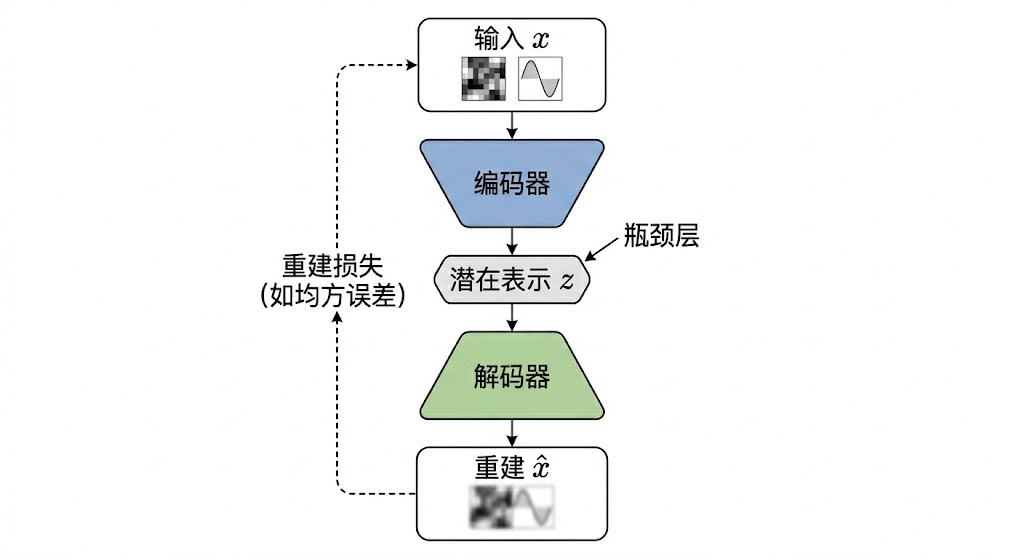
\includegraphics[width=0.8\textwidth]{fig/Autoencoders.jpg}
    \caption{自编码器结构}
    \label{fig:AE}
\end{figure}

在介绍了自编码器的数学形式后，读者可能已经注意到：潜在表示 \(z\) 的维度被有意设置得比输入 \(x\) 小得多。这种结构有一个形象的名称——“瓶颈”。

\begin{definition}[][瓶颈结构（Bottleneck Architecture）]
在自编码器中，瓶颈结构是指编码器将输入映射到一个维度远小于输入空间的潜在空间，迫使信息通过一个狭窄的“通道”。这种设计强迫网络丢弃冗余信息，只保留数据中最本质的特征，从而实现高效的压缩表示。从几何上看，瓶颈就像瓶子的细颈——所有信息必须被压缩后才能通过，然后再由解码器扩展回原始空间。瓶颈的维度决定了压缩的程度，是控制自编码器学习能力的关键超参数。
\end{definition}

正是这个瓶颈结构，让自编码器不能简单地“复制粘贴”，而必须学会提取数据中的核心规律。接下来的问题就是：如何确保网络真的学到了有用的特征，而不是通过某种取巧的方式绕过压缩？这种“压缩”真的能抓住最重要的特征吗？如果网络发现直接复制输入最省事，它会不会偷懒？另外，现实世界的数据往往充满噪声，模型怎样才能学会忽略那些无关的干扰？还有，如果我想用自编码器生成全新的、合理的数据，而不是仅仅重建已有的样本，又该怎么做？我们可以在瓶颈之外引入更多的约束，让自编码器朝着更理想的方向演化。

让我们顺着这些思考，一步步探索自编码器的改进方向。

\subsubsection*{自编码器能学到什么？从“偷懒”说起}

假设我们让自编码器学习手写数字的表示。如果潜在空间的维度与输入一样大（比如784维），网络完全可以学会一个恒等映射——直接把输入复制到输出，这样损失函数就为零了。但这样得到的“表示”毫无意义，因为它根本没有压缩任何信息。因此，我们必须迫使网络寻找更高效的信息表达方式。一个自然的方法是“限制潜在空间的维度”，让它远小于输入维度。这迫使网络必须舍弃一些冗余信息，只保留最重要的特征。

但还有没有其他方法？读者可能注意到，我们之前学习的L1正则化会让权重变得稀疏。类似的思路也可以用在自编码器上：如果我们强制潜在表示中大多数神经元为零，只允许少数几个神经元激活，那么网络就必须用这有限的几个“通道”去编码数据中的关键模式。这就引出了“稀疏自编码器”：在损失函数中加入对隐藏层输出的稀疏约束（例如L1惩罚），迫使编码更加“节俭”，从而突出最重要的特征。

\subsubsection*{当输入不干净时，自编码器还能学到本质吗？}

现实中的数据往往不完美——图片可能有噪点，文本可能有错字，传感器可能产生干扰。一个理想的自编码器应该能够抓住数据中稳定的结构，而不是被这些细小的扰动牵着鼻子走。如果我们直接让网络学习重建带噪声的输入，它可能会把噪声也当作需要保留的信息。

那么，能不能让网络学会“去噪”？一个巧妙的做法是：在输入中人为添加噪声（比如随机把一些像素置零），但要求网络重建原始的、干净的数据。这样一来，模型必须学会忽略那些随机的扰动，只关注数据中真正稳定的模式。这正是“去噪自编码器”的核心思想。它强迫网络成为一个“去噪器”，从而学到更鲁棒的特征表示。从这个角度看，去噪自编码器也是一种正则化手段——它让模型不能过于依赖输入的每一个细节，类似于我们之前学过的Dropout。

\subsubsection*{从“压缩”到“生成”：我们能创造新数据吗？}

到目前为止，自编码器做的事情都是：给定一个输入，输出一个重建。但如果读者思考得更深一点，可能会问：既然潜在空间 \(z\) 是数据的压缩表示，那么从这个空间里随机选一个点，解码器能不能生成一个合理的、从未见过的新样本？比如，从手写数字的潜在空间里取一个点，能不能生成一个看起来像手写数字的图像？

这就引出了一个更深层次的问题：我们需要知道潜在空间的分布是什么样的。在基础自编码器中，我们只学到了从 \(x\) 到 \(z\) 的映射，但不知道 \(z\) 在整个空间中的分布规律——因此无法随机采样生成新样本。为了能够“创造”新数据，研究者们提出了“变分自编码器（VAE）”。它不再学习一个固定的 \(z\)，而是学习潜在变量的概率分布（通常假设为高斯分布），让解码器学会从这个分布中采样并生成新的、与训练数据相似但不完全相同的样本。VAE不仅是一个压缩工具，更是生成模型的重要代表。

\subsubsection*{这些变体告诉我们什么？}

回顾这一路的思考，我们看到了自编码器是如何从基础的“复制-压缩”框架，一步步演变成更强大的工具的：
\begin{itemize}
\item 担心网络偷懒？——用“稀疏约束”让它必须选择最重要的特征。
\item 担心网络偷懒？——用“稀疏约束”让它必须选择最重要的特征。
\item 想生成新数据？——用“概率建模（VAE）”让它学会潜在空间的分布。
\end{itemize}

这些变体不是凭空出现的，而是研究者们在实践中发现问题、解决问题的自然产物。它们让自编码器在不同任务中各显神通：稀疏自编码器用于特征选择，去噪自编码器用于预训练和降噪，VAE用于生成图像、文本等。

在深度学习发展的早期，自编码器曾扮演过重要角色——它们被用来逐层预训练深度网络，正如我们前面提到的“逐层贪婪预训练”。随着数据量和计算能力的增长，这种预训练方式虽然逐渐被端到端的训练取代，但自编码器本身所蕴含的思想（学习压缩表示、对抗噪声、生成新数据）依然深刻地影响着后续的模型设计。特别是我们即将学习的卷积神经网络，它的许多核心思想（如层次化特征学习）都可以在自编码器的框架下找到影子。

\subsection{卷积神经网络（Convolutional Neural Network, CNN）}
\begin{remark}
在上一节中，我们学习了自编码器如何通过瓶颈结构学习数据的压缩表示。对于图像数据，自编码器也能处理，只需将图像像素展平成向量，然后送入全连接层。但读者可能会注意到一个严重的问题：一张$224\times 224$ 的图像，展开后就有5万多个维度，如果直接用全连接层，光是第一层的参数就可能高达几百万甚至几十亿。这不仅计算量惊人，还容易导致过拟合。更重要的是，把像素强行拉直会丢失图像的空间结构——相邻像素之间的位置关系，对图像理解至关重要。

那么，有没有一种方法既能保留空间结构，又能大幅减少参数？这就要回到图像本身的特性：一幅图像中，重要的往往是局部模式，比如边缘、角点、纹理。而且这些模式出现在图像的不同位置时，本质上是一样的。例如，一只猫的耳朵可能出现在左上角，也可能在右下角，但识别耳朵所需的“检测器”应该是相同的。这些观察，正是卷积神经网络（Convolutional Neural Network, CNN）的设计根基。
\end{remark}

传统全连接层中，每个神经元与上一层所有神经元相连，相当于用一个巨大的矩阵去捕捉全局关系。而卷积网络换了一个思路：每个神经元只与输入的一小块区域连接，这一小块区域称为感受野。这样，模型首先学习到的是局部的模式，比如边缘、纹理。然后，随着层数加深，将局部模式组合成更高级的特征，比如形状、物体部件。

这种“局部连接”大大减少了参数数量。假设输入是 \(224\times224\) 的图像，如果用 \(3\times3\) 的卷积核，每个卷积核只有9个参数，而不是全连接层的数万个参数。更重要的是，由于图像中同一模式可能出现在任何位置，我们让同一个卷积核在整个图像上滑动，即权重共享。这样一来，无论耳朵出现在哪里，同一个检测器都能起作用。这种设计天然赋予模型平移不变性——物体在图像中移动，网络依然能识别。

在理解了CNN的设计理念之后，我们来看看它最核心的操作——卷积。这个操作正是“局部连接”和“权重共享”在数学上的具体实现。

\begin{definition}[][卷积（Convolution）]
在卷积神经网络中，卷积是指用一个小型可学习的权重矩阵（称为卷积核或滤波器）在输入数据上滑动，计算窗口内元素与卷积核对应位置的加权和。对于二维图像输入 \(I\) 和卷积核 \(K\)（大小为 \(m \times n\)），输出特征图在位置 \((i,j)\) 的值定义为：
\[(I * K)_{i,j} = \sum_{p=0}^{m-1} \sum_{q=0}^{n-1} I_{i+p, j+q} \cdot K_{p,q}\]
这个运算可以理解为：卷积核在输入上滑动，每到一个位置，就将其覆盖的区域与核做逐元素相乘并求和，得到一个输出值。通过使用多个不同的卷积核，网络可以学习到多种局部特征（如边缘、纹理、角点）。
\end{definition}
卷积操作具有以下关键特性：
\begin{itemize}
    \item 局部连接：每个输出单元只与输入的一小块区域相连，减少了参数数量。
    \item 权重共享：同一个卷积核在整张图像上滑动，参数被重复使用，进一步压缩参数量，并使模型具有平移不变性。
\end{itemize}
但一个卷积核只能检测一种模式（比如垂直边缘），而图像中往往需要几十甚至上百种不同的特征。因此，实际应用中我们会同时使用多个卷积核，每个核生成一张特征图（feature map）。这些特征图堆叠在一起，就构成了卷积层的输出。每个卷积核都是可学习的，网络在训练过程中会自己发现哪些特征对当前任务最重要。得到特征图后，通常还会紧跟着一个非线性激活函数（比如ReLU），为模型引入非线性，这与我们之前学习的全连接网络中的激活函数作用相同。

\subsubsection{卷积层}

卷积层是CNN的基础构建块。它接收输入（可能是原始图像，也可能是上一层的特征图），用一组可学习的卷积核在输入上滑动，计算每个位置的加权和。数学上，对于一个输入 \(I\) 和卷积核 \(K\)（大小为 \(m\times n\)），输出特征图中位置 \((i,j)\) 的值为：
\[
(I * K)_{i,j} = \sum_{p=0}^{m-1} \sum_{q=0}^{n-1} I_{i+p, j+q} \cdot K_{p,q}
\]
这一运算可以理解为：卷积核在输入上从左到右、从上到下依次滑动，每到一个位置，就把覆盖区域与核做逐元素相乘并求和，得到一个输出值。通常，我们会同时使用 \(C_{\text{out}}\) 个不同的卷积核，因此卷积层的输出是一个 \(C_{\text{out}}\) 个通道的特征图，每个通道对应一种检测到的特征。

在实际实现中，还需要指定步长（stride）和填充（padding）。步长控制卷积核每次滑动的像素数，步长越大，输出尺寸越小；填充则是在输入边界周围补零，使得输出尺寸能够保持或仅略微缩小，同时也能让卷积核覆盖到边缘像素。

\subsubsection{池化层}

在卷积层之后，通常会加入池化层（pooling layer）。它的主要作用是降低特征图的尺寸，从而减少后续层的参数数量和计算量，同时也能增强模型对微小位移的鲁棒性——这正是我们之前提到的平移不变性。池化层在输入上滑动一个窗口（通常是 \(2\times2\)），对窗口内的值进行聚合，常见的聚合方式有：
\begin{itemize}
\item 最大池化：取窗口内的最大值。它能保留窗口中最显著的特征，抑制非极大值，从而增强特征的不变性。
\item 平均池化：取窗口内的平均值。它更能保留整体的背景信息，但在图像分类任务中通常不如最大池化常用。
\end{itemize}
例如，对于一个 \(2\times2\) 的窗口，最大池化会输出窗口内四个数的最大值；如果步长也为2，那么输出尺寸就会减半。这种下采样操作极大地降低了后续层的计算量，同时也让网络对小的位置变化不再敏感。

\subsubsection{全连接层}

经过若干卷积层和池化层的逐级抽象后，特征图已经变得非常“高级”——例如，在图像分类任务中，最后的特征图可能已经能捕捉到物体的类别信息。这时，我们需要将这些二维特征图转换为一维向量，然后送入一个或多个全连接层（fully connected layer），完成最终的分类或回归。全连接层就是我们之前学习的普通神经网络层，每个神经元与上一层的所有输出相连。在输出层，通常使用Softmax函数将得分转换为概率分布，这与多分类任务的输出层设计完全一致。

\begin{figure}[htbp]
    \centering
    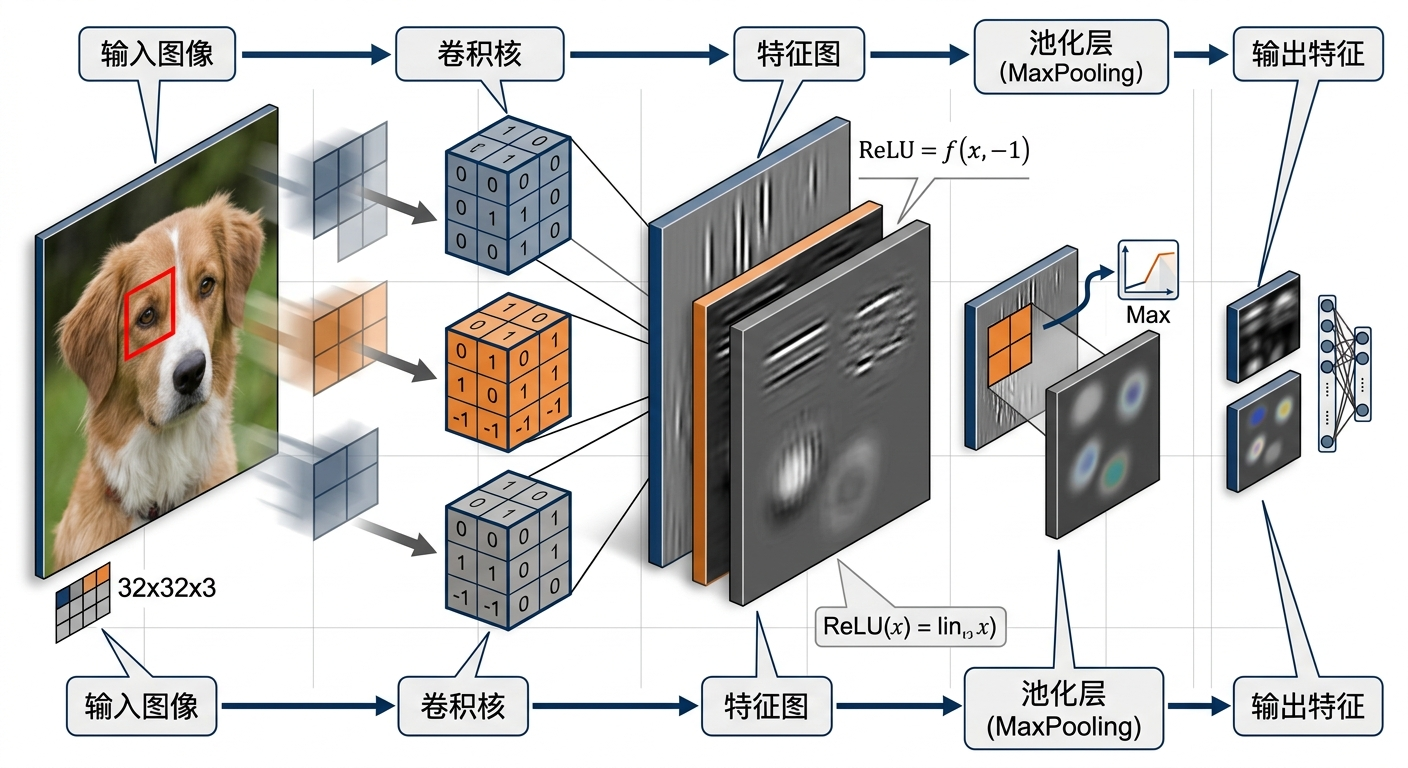
\includegraphics[width=0.8\textwidth]{fig/cnn.jpg}
    \caption{卷积神经网络}
    \label{fig:cnn}
\end{figure}

\subsubsection{经典架构的演进}

自2012年AlexNet在ImageNet竞赛中一战成名后，研究者们开始思考一个朴素的问题：如果网络更深，性能会不会更好？这个念头驱使着人们不断探索更深、更复杂的架构。

最初，AlexNet证明了深度（8层）加上ReLU、Dropout和GPU训练，就能在图像识别上碾压传统方法。但它的成功也留下了一个开放的问题：能不能再深一点？VGG（2014）给出了肯定的答案——它用统一的3×3小卷积核堆叠出16～19层的网络，结构简洁规整，在保持参数量可控的前提下，进一步提升了性能。然而，VGG也暴露了深度的代价：随着层数增加，训练变得异常缓慢，且梯度消失的问题再次浮现，尤其是当网络超过20层时，反向传播的信号已经很难到达浅层。

于是，研究者们不得不直面一个看似矛盾的现象：深度是提升性能的关键，但过深的网络却难以训练。2015年，微软亚洲研究院的何恺明团队提出了ResNet，给出了一个优雅的解决方案——他们不再让网络直接学习原始的映射，而是学习残差：让网络拟合恒等映射与原始目标之间的差值，并引入跳跃连接（skip connection）将输入直接加到输出上。这样一来，梯度可以沿着跳跃连接直接传递到浅层，彻底解决了梯度消失问题。ResNet成功训练出152层的网络，将ImageNet错误率降到了3.6\%，超越了人类水平。

从AlexNet到VGG再到ResNet，这条演进路径清晰地揭示了一个规律：每次架构突破，本质上都是在解决“如何让网络更深”这个核心难题。而解决过程中，我们之前学到的ReLU、Dropout、正则化等技术，都成了这些经典架构的必备组件。

现在，我们学习了卷积神经网络如何利用“局部连接”和“权重共享”高效处理图像这类空间结构数据。但现实中还有另一类重要的数据，它们的结构不是空间上的，而是时间上的。比如一段文字，单词的先后顺序决定了句子的含义；一段语音，音节的时序关系承载着信息；一段股价走势，历史数据影响着未来的预测。这类数据被称为序列数据，处理它们的关键在于：模型需要具备记忆能力——它必须能够记住前面看到的内容，并利用这些信息影响对后续输入的判断。

这正是循环神经网络（Recurrent Neural Network, RNN）的设计初衷。它通过引入一个“隐藏状态”来充当记忆，让网络能够沿着时间轴传递信息。

\subsection{循环神经网络（RNN）}

\begin{remark}
想象你在读一句话：“我今天去了……，因为想买点水果。”要猜出“……”是什么，你需要记住前面说的是“去了”某个地方，而这个地方通常与买水果相关。
\end{remark}
传统的前馈网络没有这种“记住前面”的能力——每个输入都是独立处理的。RNN则通过一种巧妙的设计解决了这个问题：它在每一时刻都会把上一时刻的“记忆”传递过来，与当前输入一起决定当前输出。从数学上看，RNN的状态更新公式为：
\[
h_t = \tanh(W_{hh}h_{t-1} + W_{xh}x_t + b_h)
\]
这里：
\begin{itemize}
\item $h_{t-1}$ 是上一时刻的记忆，$W_{hh}$ 是记忆如何影响当前时刻的权重；
\item $x_t$ 是当前输入，$W_{xh}$ 是输入如何影响当前时刻的权重；
\item $\tanh$ 激活函数将结果压缩到 $(-1,1)$ 之间，使数值稳定；
\item 最终的输出通常由 $h_t$ 经过另一个全连接层得到。
\end{itemize}

\begin{figure}[htbp]
    \centering
    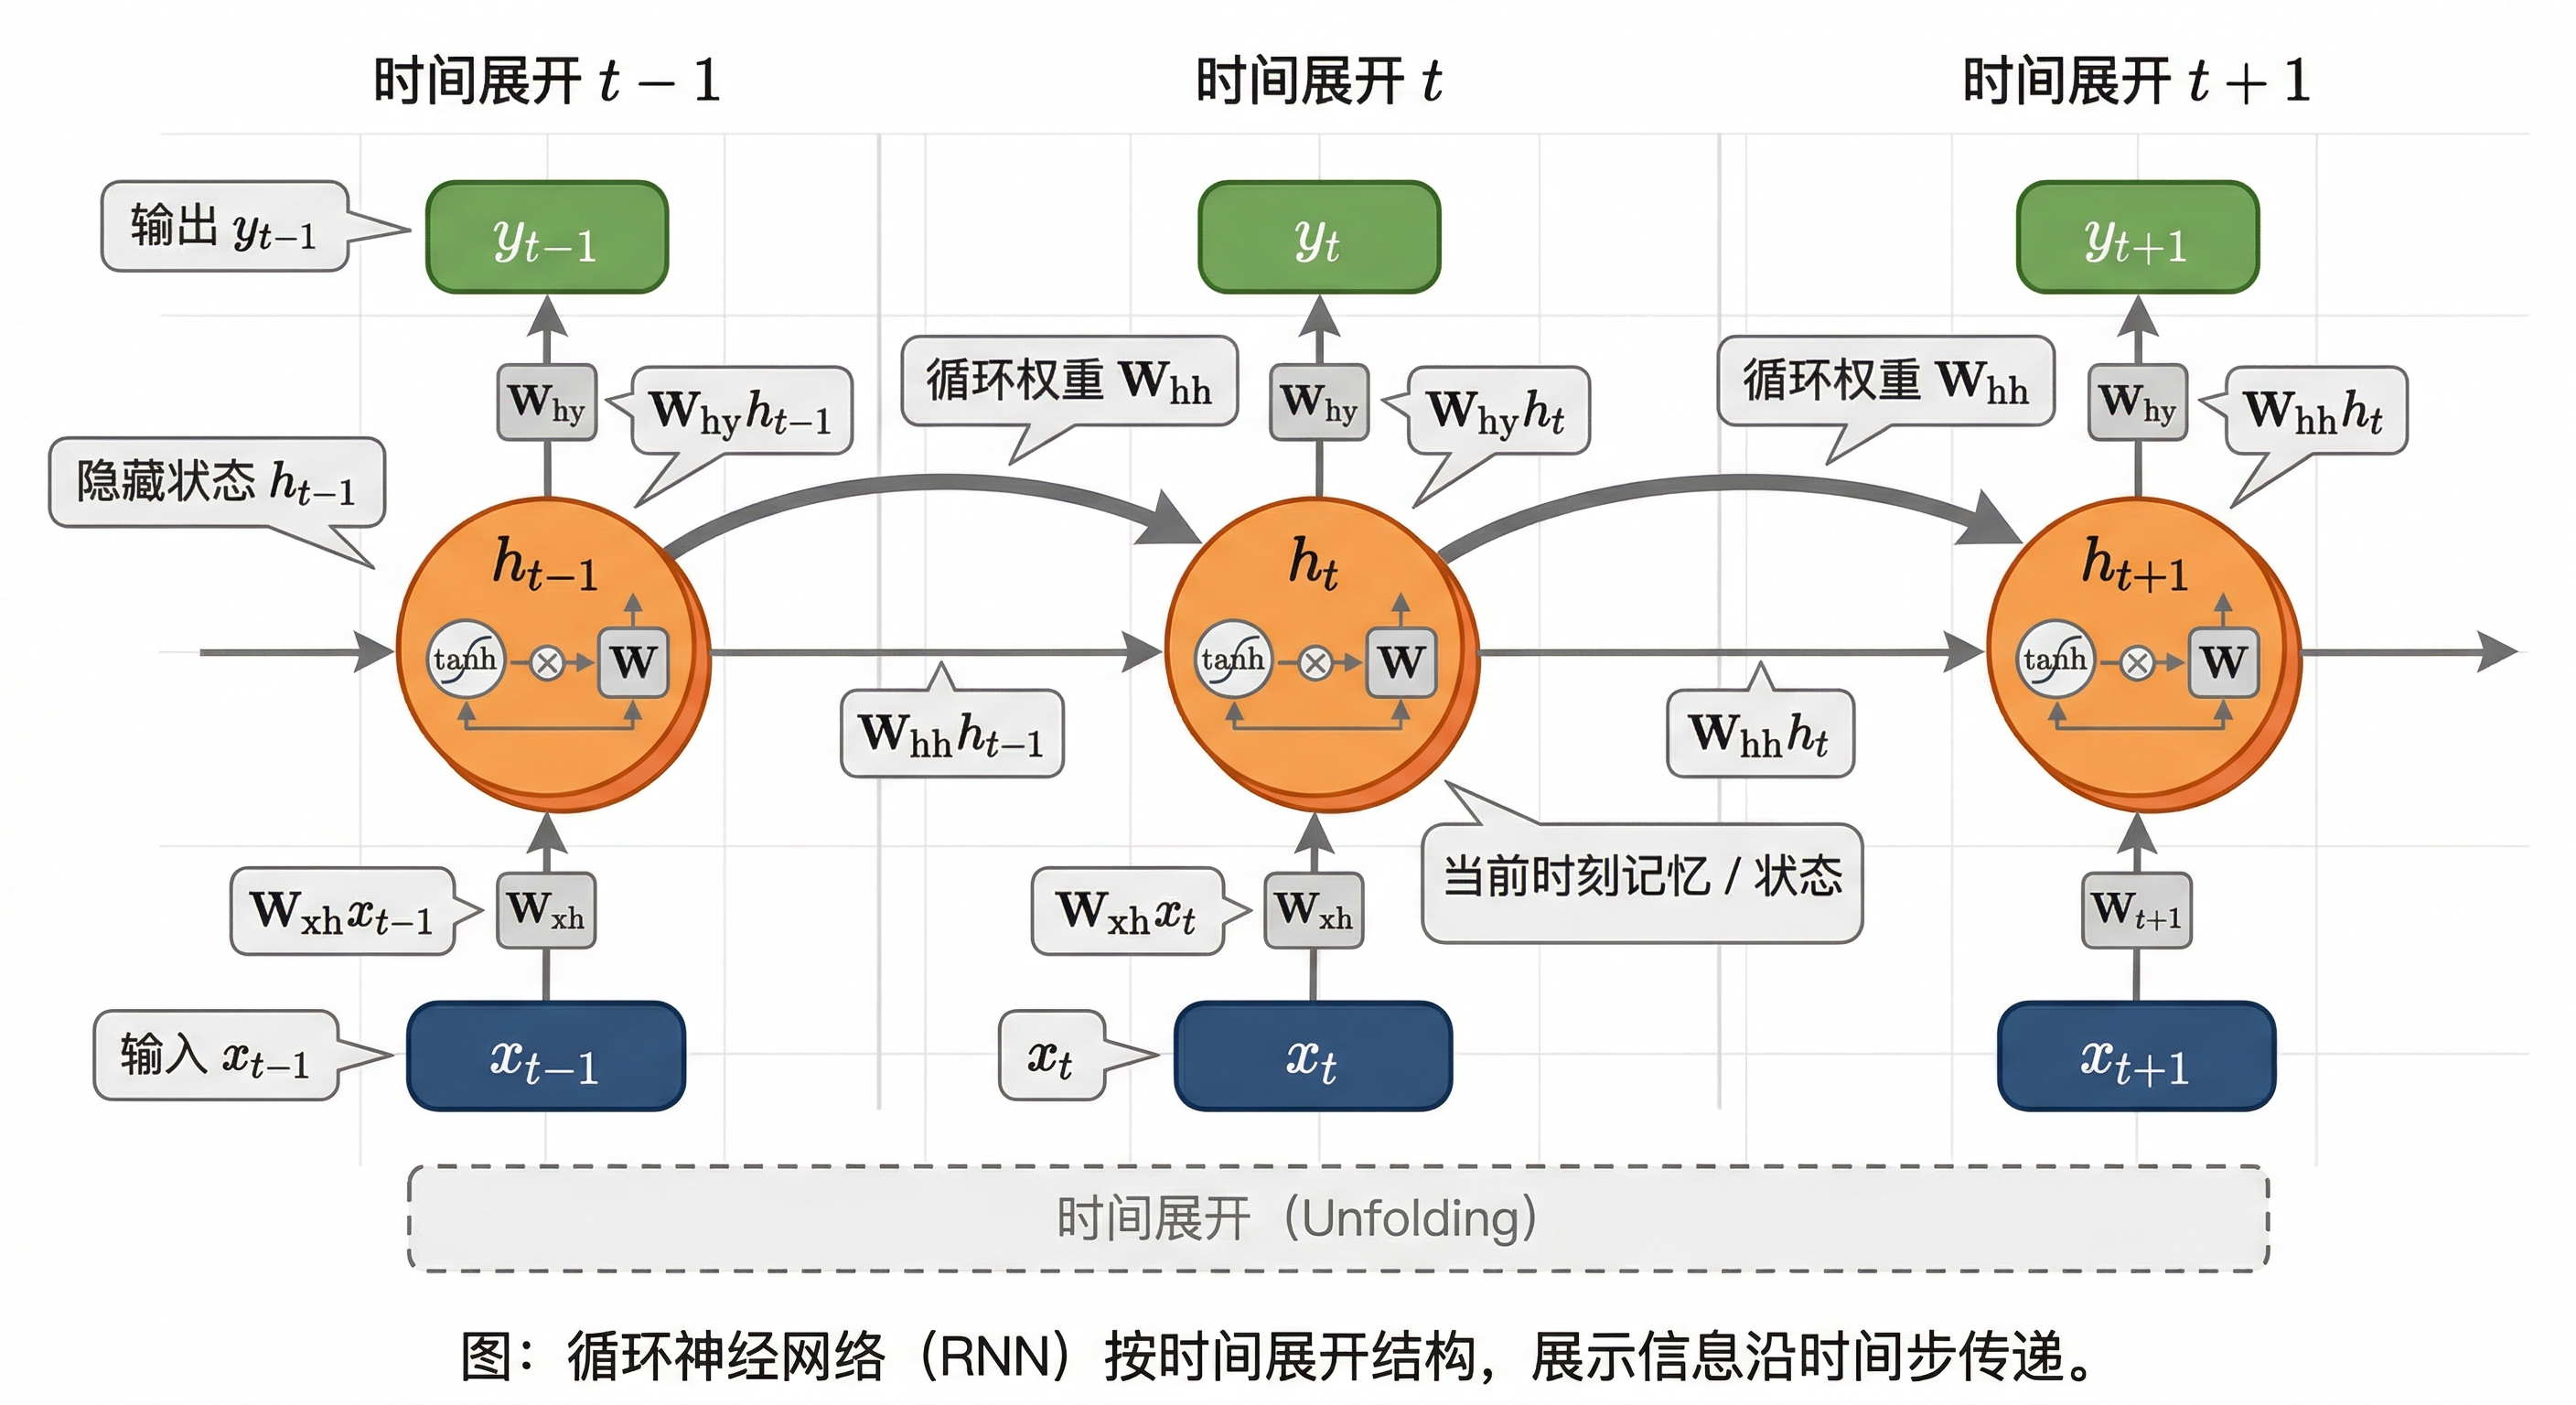
\includegraphics[width=0.8\textwidth]{fig/rnn.jpg}
    \caption{循环神经网络}
    \label{fig:rnn}
\end{figure}

\subsubsection{RNN的困境：梯度消失与长期依赖}

理论上，RNN可以记住很久以前的信息——因为隐藏状态会沿着时间链一直传递下去。但实践中，标准RNN很难学习到超过10步的依赖关系。这是什么原因呢？

读者可能还记得，在深层前馈网络中，梯度消失是由链式法则连乘导致的。RNN在时间上展开后，本质上就是一个\textbf{时间上的深层网络}——每一时刻相当于一层，时间越长，网络越深。在反向传播时，误差信号需要沿着时间链往回传播，每经过一个时间步就要乘上一个 $\tanh$ 的导数（通常小于1）。经过几十步的连乘，梯度就会指数级衰减，使得早期时刻的记忆几乎无法被更新。

这个现象被称为\textbf{长期依赖问题}。它意味着标准RNN虽然能记住几秒内的信息，但对于更长的序列（如一段话或一篇文档）往往力不从心。例如，要让RNN根据文章开头的一句话“他在北京出生”，去预测结尾处“所以他很爱吃……”，模型需要跨越大量文本，把“北京”这个信息保留到最后——这对标准RNN来说是个巨大挑战。

\subsubsection{从RNN到LSTM：门控机制的引入}

为了解决长期依赖问题，研究者们设计了更精巧的循环单元，其中最著名的是\textbf{长短时记忆网络（Long Short-Term Memory, LSTM）}。LSTM的核心思想是：让网络自己学会“什么该记住，什么该忘记，什么该输出”。它通过引入三个\textbf{门控}（输入门、遗忘门、输出门）来精细控制信息的流动，使得重要信息可以在记忆单元中长期保存，不受梯度消失的干扰。

LSTM的出现，让循环神经网络真正具备了处理长序列的能力，在机器翻译、语音识别、文本生成等领域大放异彩。在下一节中，我们将深入拆解LSTM的内部结构，看看这些“门”是如何协同工作的，以及它们如何让记忆变得“长效”。

\subsection{LSTM：长短期记忆网络}

LSTM是由Hochreiter和Schmidhuber在1997年提出的，它通过引入一个精巧的“门控”机制，让网络自己学会管理记忆。就像我们的大脑会判断“这条信息重要，要记住”，“那条信息过时了，该忘掉”，“当前场景下我应该输出什么”，LSTM的每个门都是一个带有Sigmoid激活函数的子网络，输出0到1之间的数值，用来控制信息通过的比例。0表示“完全不让通过”，1表示“全部让通过”。

让我们一步步拆解LSTM的内部结构。假设当前时刻的输入是 \(x_t\)，上一时刻的隐藏状态是 \(h_{t-1}\)，上一时刻的“记忆”是 \(C_{t-1}\)（LSTM中专门有一个称为细胞状态的通道，用来长期保存信息）。LSTM会依次执行三个操作：
\begin{enumerate}
    \item 遗忘门：决定从细胞状态中丢弃什么信息。它看着 \(h_{t-1}\) 和 \(x_t\)，输出一个0到1之间的值给细胞状态中每个元素，1表示“完全保留”，0表示“完全遗忘”。
   \[
   f_t = \sigma(W_f \cdot [h_{t-1}, x_t] + b_f)
   \]
   比如在处理文本时，遗忘门可能会判断“前一句话的主语已经不再重要，该忘掉了”。
   \item 输入门：决定将哪些新信息存入细胞状态。它包含两个部分：一个Sigmoid层决定哪些值要更新（输入门），一个tanh层生成候选值 \(\tilde{C}_t\)，然后两者相乘，得到要添加到细胞状态的新信息。
   \[i_t = \sigma(W_i \cdot [h_{t-1}, x_t] + b_i) ,~~\tilde{C}_t = \tanh(W_C \cdot [h_{t-1}, x_t] + b_C)\]
   例如，读到一个新名词“李华”，输入门可能会决定把这个新信息存入记忆。
   \item 细胞状态更新：结合遗忘门和输入门，更新旧的细胞状态 \(C_{t-1}\)：
   \[
   C_t = f_t \odot C_{t-1} + i_t \odot \tilde{C}_t
   \]
   这里 \(\odot\) 表示逐元素相乘。这个公式直观地表达了：我们保留一部分旧记忆（ \(f_t \odot C_{t-1}\) ），再加入一部分新信息（ \(i_t \odot \tilde{C}_t\) ）。
   \item 输出门：决定基于当前的细胞状态输出什么。首先用Sigmoid层决定哪些部分会被输出，然后将细胞状态通过tanh压缩到-1到1之间，再与输出门相乘，得到最终的隐藏状态 \(h_t\)。
   \[o_t = \sigma(W_o \cdot [h_{t-1}, x_t] + b_o) ,~~ h_t= o_t \odot \tanh(C_t)\]
   输出门就像一个“过滤器”，决定当前场景下哪些记忆应该被表达出来。例如，在预测下一个词时，可能只需要输出与当前语境相关的部分记忆。
\end{enumerate}

\begin{figure}[htbp]
    \centering
    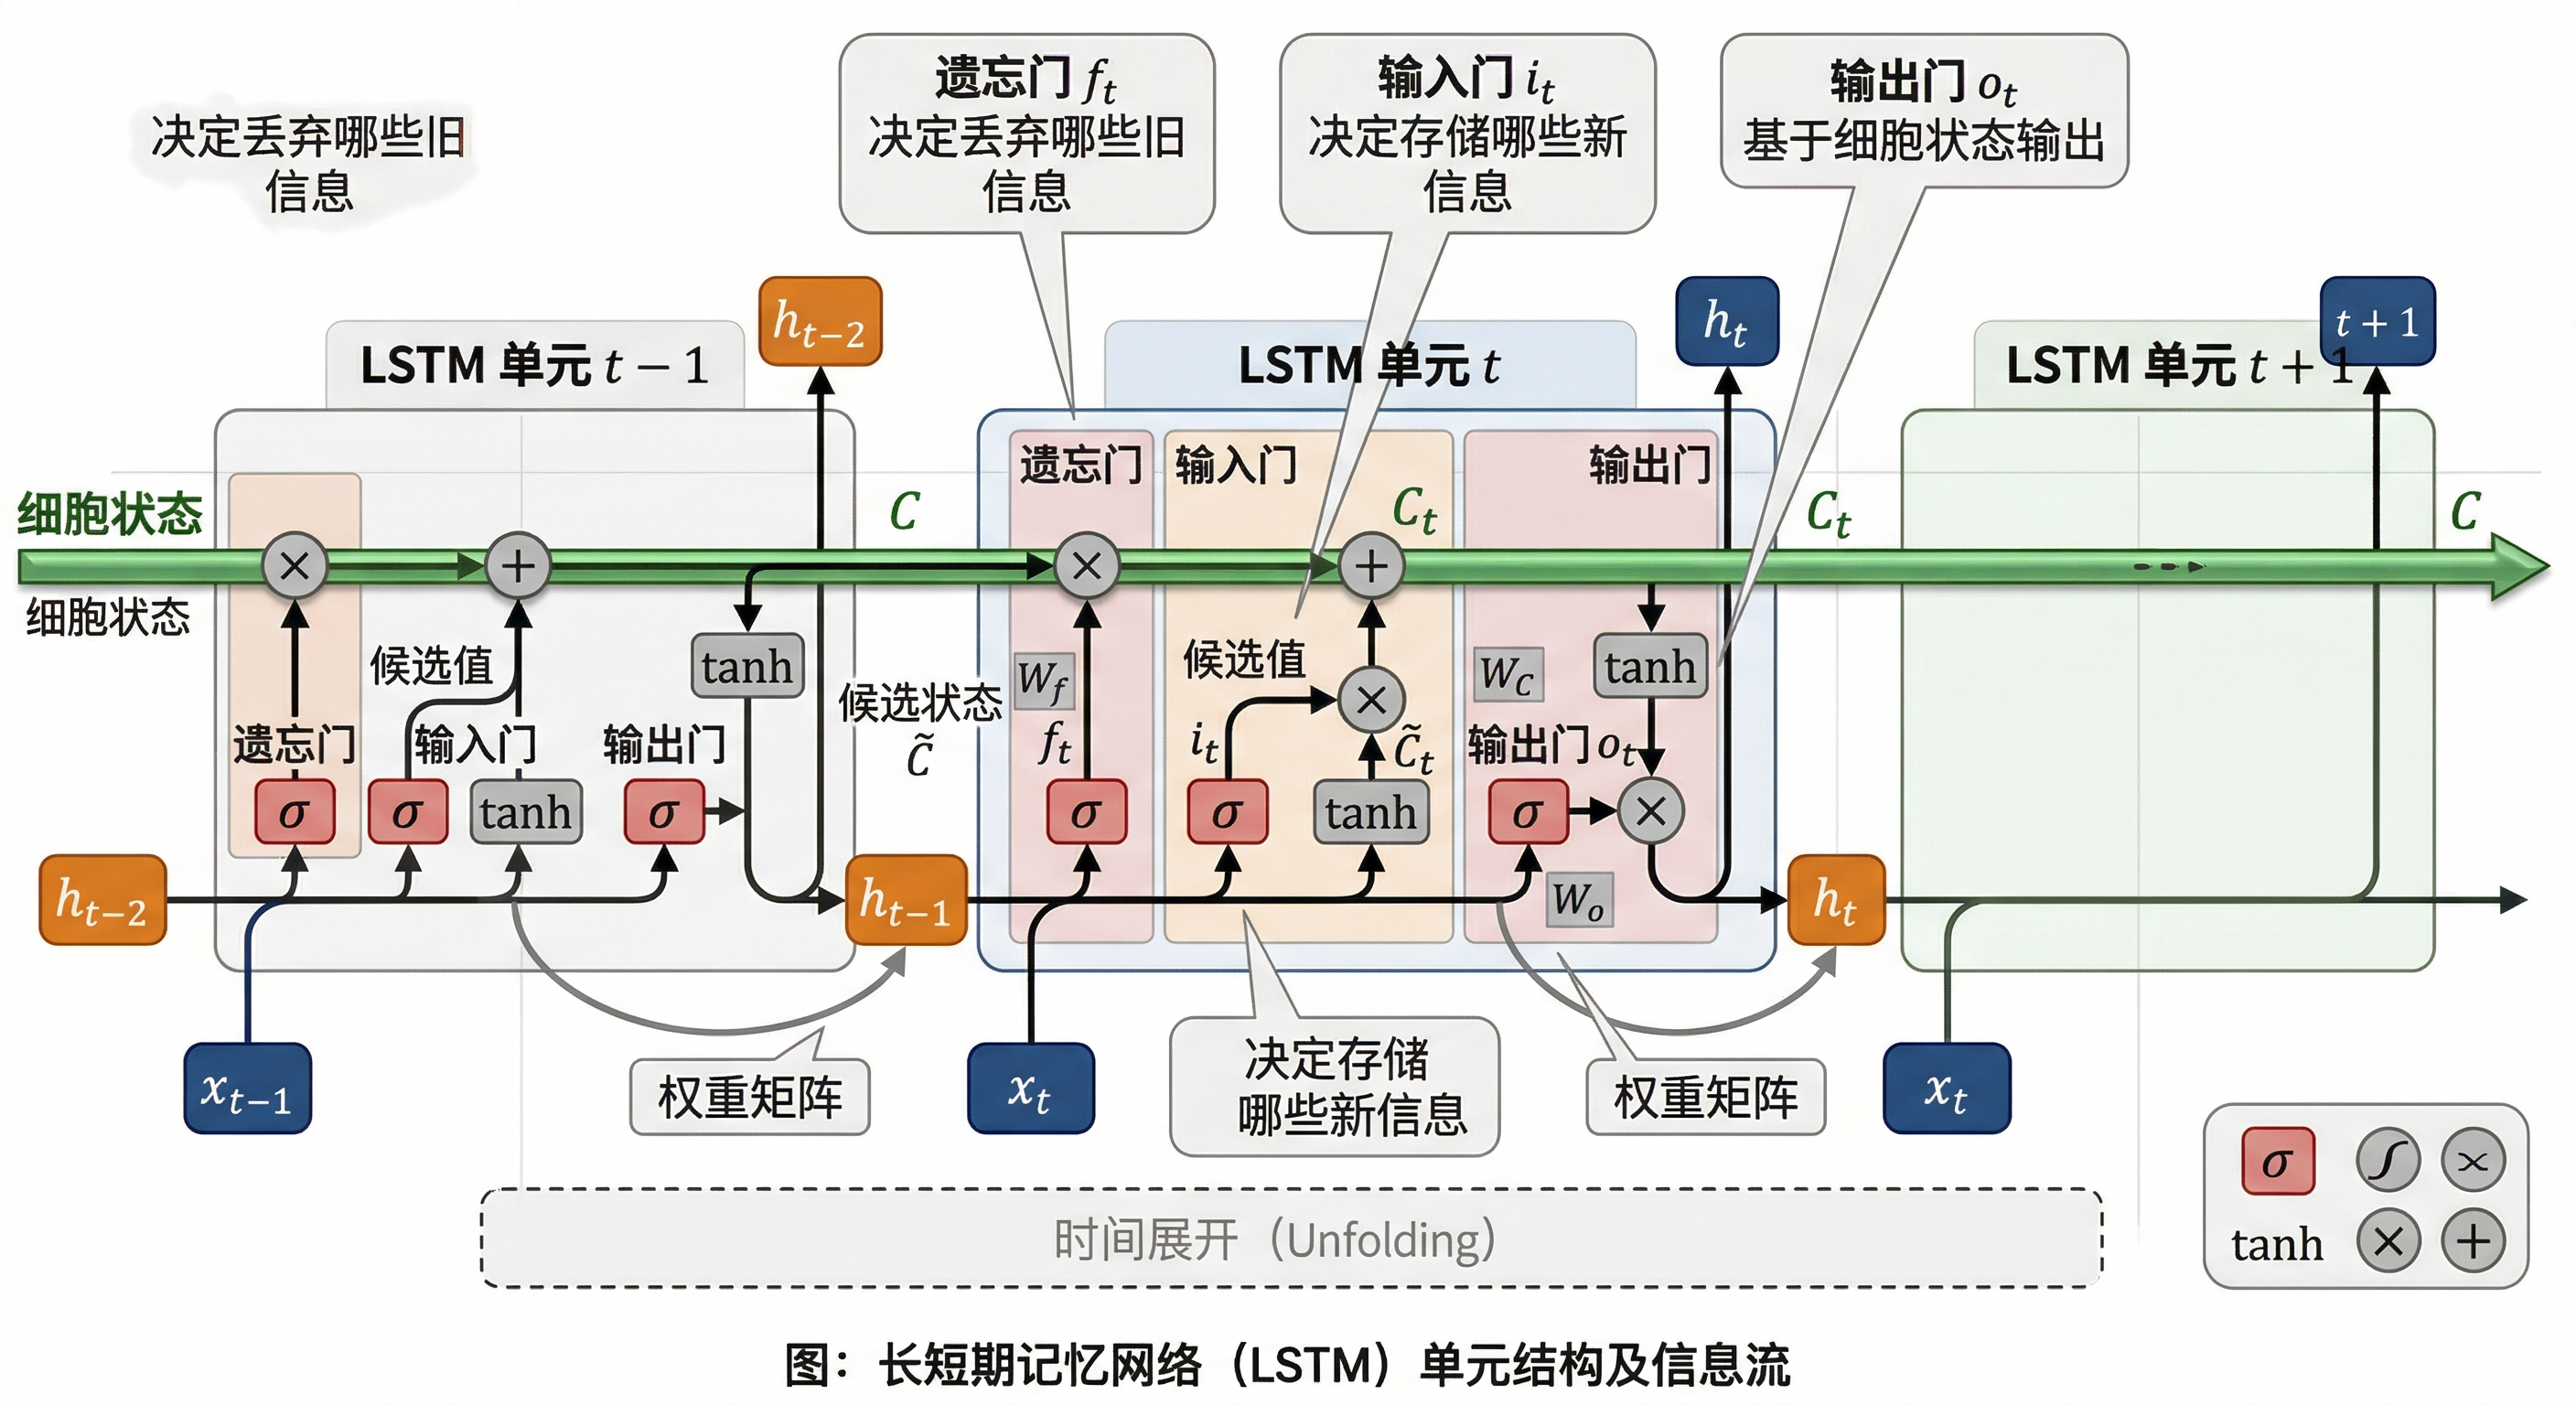
\includegraphics[width=0.95\textwidth]{fig/LSTM.jpg}
    \caption{长短期记忆网络}
    \label{fig:LSTM}
\end{figure}

\subsection{生成对抗网络（GANs）}

在上一节中，我们学习了LSTM如何通过门控机制捕获序列中的长期依赖关系。这类模型擅长处理已有的数据——给定一段文字，它可以翻译成另一种语言；给定一段语音，它可以转写成文本。但读者可能会想：有没有一种模型不仅能理解数据，还能创造出全新的、以假乱真的数据？比如，能不能让模型自己画出一张从来没有人画过的猫的图片，或者写出一段从来没有出现过的优美句子？

这正是生成式模型的研究目标。而在众多生成式模型中，最引人注目的当属生成对抗网络（Generative Adversarial Networks, GANs）。它用一种充满博弈智慧的方式，让两个网络相互对抗、共同进化，最终学会生成极其逼真的数据。

\begin{remark}
想象一个场景：有一个造假币的团伙（生成器），他们试图制造出能以假乱真的假币；与此同时，警方有一个鉴别团队（判别器），他们不断训练自己识别假币。造假者每制造一批假币，鉴别师就指出哪些地方露出了马脚；造假者根据反馈改进工艺，生产出更逼真的假币；鉴别师也同时提升自己的鉴别能力……如此循环往复，最终造假者制造的假币足以骗过最专业的鉴别师。
\end{remark}
这正是GANs的核心思想。它由两个神经网络组成：
\begin{itemize}
\item 生成器（Generator, \(G\)）：输入一个随机噪声向量 \(z\)（可以理解为“创意种子”），输出一个伪造样本，比如一张“猫”的图片。它的目标是让生成的样本尽可能逼真，骗过判别器。
\item 判别器（Discriminator, \(D\)）：输入一个样本（可能是真实数据，也可能是生成器生成的假数据），输出一个概率，表示这个样本是真实数据的可能性。它的目标是尽可能准确地区分真假。
\end{itemize}
这两个网络的目标完全相反：生成器想方设法欺骗判别器，判别器则努力不被骗。这种对抗关系在数学上被形式化为一个\textbf{极小极大博弈}（minimax game）问题：
\[
\min_G \max_D V(D, G) = \displaystyle\mathbb{E}_{x \sim p_{\text{data}}(x)}[\log D(x)] + \mathbb{E}_{z \sim p_z(z)}[\log(1 - D(G(z)))]
\]
这个式子可能看起来有点复杂，但它的含义很直观：
\begin{itemize}
\item  第一项 \(\mathbb{E}_{x \sim p_{\text{data}}(x)}[\log D(x)]\) 表示判别器对真实数据的判断——它希望给真实数据打高分（\(D(x)\) 接近1），这样 \(\log D(x)\) 就接近0（负值很小）。
\item  第二项 \(\mathbb{E}_{z \sim p_z(z)}[\log(1 - D(G(z)))]\) 表示判别器对生成数据的判断——它希望给假数据打低分（\(D(G(z))\) 接近0），这样 \(\log(1 - D(G(z)))\) 也接近0。
\item  判别器 \(D\) 希望最大化整个表达式，即让真实数据得分高、假数据得分低。
\item  生成器 \(G\) 希望最小化这个表达式，即让假数据也能得高分，从而骗过判别器。
\end{itemize}

GANs的训练过程正是这个博弈的逐步求解：

\begin{enumerate}
    \item 训练判别器：固定生成器 \(G\) 不动，从真实数据中采样一批样本 \(x\)，从噪声中采样一批 \(z\)，生成一批假样本 \(G(z)\)。然后训练判别器 \(D\)，让它在真实样本上输出高概率，在假样本上输出低概率。这一步相当于让鉴别师学会分辨当前最逼真的假币。
    \item 训练生成器：固定判别器 \(D\) 不动，采样新的噪声 \(z\)，生成假样本，然后用判别器的输出来更新生成器。具体来说，生成器的目标是让 \(D(G(z))\) 尽可能大（即骗过判别器），因此它的损失函数是 \(-\log D(G(z))\)（或者 \(\log(1-D(G(z)))\) 的最小化）。这一步相当于让造假者根据鉴别师的反馈改进工艺。
\end{enumerate}
这两个步骤交替进行。随着训练推进，生成器越来越擅长生成逼真的样本，判别器也越来越难以分辨真假。理想情况下，两者会达到一种均衡：生成器生成的样本与真实数据分布完全一致，判别器对任何样本的判断概率都是0.5（即完全无法区分）。

\subsubsection*{GANs的力量与挑战}

自2014年Goodfellow等人提出GANs以来，它迅速成为生成式模型中最具影响力的框架之一。从生成逼真的人脸（如StyleGAN），到图像风格迁移，再到超分辨率重建和药物分子设计，GANs的应用几乎遍布人工智能的各个领域。这种成功让人不禁感叹：一个如此简洁的对抗框架，为何能迸发出如此强大的创造力？

但当我们尝试自己训练一个GAN时，往往会被现实泼一盆冷水。读者可能会发现，生成器有时会“偷懒”——它只学会生成少数几种样本，比如不管输入什么随机噪声，都只画出同一只猫，只是角度略有不同。这种现象被称为\textbf{模式崩塌}。为什么会这样？因为判别器只关心真假，不关心多样性。如果生成器能稳定地骗过判别器，它就没有动力去覆盖整个数据分布，只抓住最容易欺骗判别器的“安全区”。

另一个常见问题是训练过程中的剧烈震荡。读者可以想象，两个网络互为对手，一方变强就会迫使另一方快速追赶，如此循环。这种“你追我赶”可能导致损失函数上下波动，难以收敛。有时候判别器进步太快，生成器永远追不上；有时候生成器猛然“反超”，判别器又失去了辨别能力。这种不稳定性使得GAN的训练就像走钢丝，需要精细地平衡双方的强度。

更棘手的是，我们如何判断生成器学到了“好”的分布？传统分类任务可以用准确率、损失值来量化性能，但对于生成的图像，我们往往只能凭肉眼观察。一张模糊的图可能看起来比一张清晰但内容重复的图更“真实”，这让模型选择变得主观。即使损失值在下降，生成的样本也不一定在变好——这就是\textbf{评估困难}，至今仍是GAN领域的一大难题。

面对这些挑战，研究者们提出了大量改进方案，比如改进损失函数（WGAN）、加入正则化（梯度惩罚）、设计更稳定的网络结构（SN-GAN）等。这些努力让GANs逐渐变得更加可控和实用。但无论如何，GANs所蕴含的博弈思想依然迷人——它让模型自己学会创造，并在与对手的对抗中不断进化。在后续章节中，我们将深入探索这些改进方法，并了解GANs与其他生成模型（如变分自编码器、扩散模型）的异同。

\begin{figure}[htbp]
    \centering
    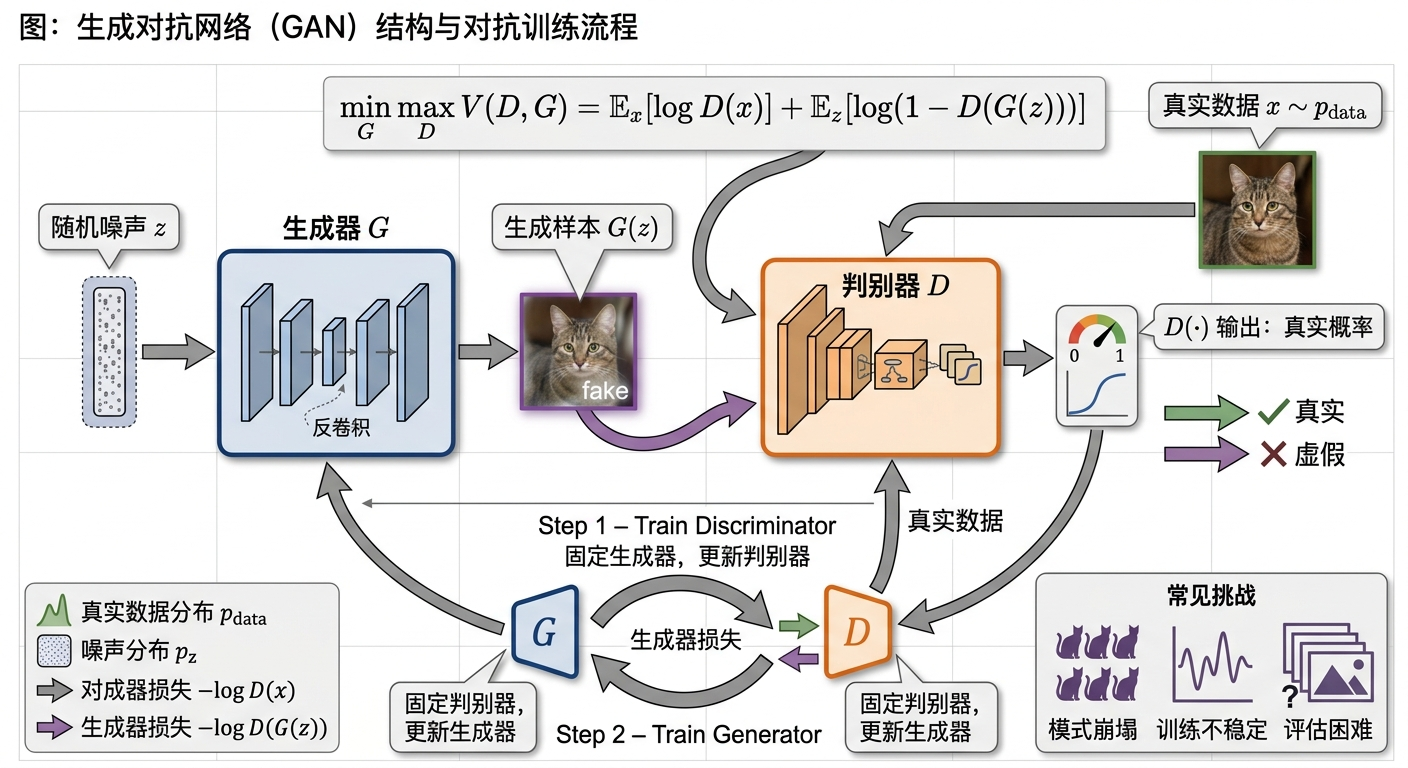
\includegraphics[width=0.95\textwidth]{fig/GAN.jpg}
    \caption{生成对抗网络}
    \label{fig:GAN}
\end{figure}

\subsection{扩散模型（Diffusion Models）}

在上一节中，我们了解了生成对抗网络（GAN）如何通过两个网络的博弈来生成逼真的数据。然而，GAN 的训练往往不稳定，容易出现模式崩塌，且需要精细地平衡生成器与判别器的能力。这让研究者们开始寻找更稳定、更可控的生成方法。一种被称为扩散模型（Diffusion Models）的新范式，在近年来异军突起，它以优雅的数学基础、稳定的训练过程和顶尖的生成质量，成为了图像生成领域的又一里程碑。你可能已经听说过由扩散模型驱动的图像生成工具，比如 DALL·E、Midjourney、Stable Diffusion——它们背后都离不开扩散模型的思想。

\begin{remark}
想象你有一张清晰的照片。现在，你反复在上面添加微小的噪声，每加一次，照片就变得更模糊一点。经过足够多次后，这张照片变成了完全随机的雪花点——你已经无法辨认出原来的内容。这个过程是**前向扩散过程**，它是有方向的：从清晰的图像逐步走向纯粹的噪声。

反过来，如果我们能学会这个过程的逆过程——从一张随机的噪声图像，一步步去除噪声，最终还原出原始的清晰图像——那我们就拥有了一个生成模型。因为我们可以先从纯噪声出发，通过逆向去噪，创造出全新的、从未见过的图像。这就是扩散模型的核心思想。
\end{remark}

\subsubsection{前向过程：逐渐加噪}

前向过程是一个固定的马尔可夫链，它逐步向数据添加高斯噪声。设原始数据为 \(x_0\)，经过 \(T\) 步后，得到纯噪声 \(x_T\)。每一步的转换定义为：
\[
q(x_t | x_{t-1}) = \mathcal{N}(x_t; \sqrt{1-\beta_t} x_{t-1}, \beta_t I)
\]
这里 \(\beta_t \in (0,1)\) 是一个预定义的噪声调度（通常很小的值，比如 0.0001 到 0.02），控制每一步添加噪声的强度。\(\mathcal{N}(\mu, \sigma^2 I)\) 表示均值为 \(\mu\)、协方差矩阵为 \(\sigma^2 I\) 的高斯分布。简单来说，\(x_t\) 就是在 \(x_{t-1}\) 的基础上加上一点点随机噪声，并适当缩小幅值，使得最终方差可控。

一个重要的性质是，我们可以直接从 \(x_0\) 一步计算出任意 \(t\) 时刻的带噪声数据，而不需要一步步迭代：
\[
x_t = \sqrt{\bar{\alpha}_t} \, x_0 + \sqrt{1 - \bar{\alpha}_t} \, \epsilon
\]
其中 \(\alpha_t = 1 - \beta_t\)，\(\bar{\alpha}_t = \prod_{i=1}^t \alpha_i\)，\(\epsilon \sim \mathcal{N}(0, I)\)。这极大地方便了训练。

\subsubsection{反向过程：学习去噪}

前向过程是固定的，而反向过程是我们需要学习的。我们的目标是训练一个神经网络 \(p_\theta\)，它能从噪声图像中逐步恢复出原始数据。反向过程也定义为一个马尔可夫链：
\[
p_\theta(x_{t-1} | x_t) = \mathcal{N}(x_{t-1}; \mu_\theta(x_t, t), \Sigma_\theta(x_t, t))
\]
也就是说，给定当前时刻的噪声图像 \(x_t\)，网络预测上一个时刻的均值 \(\mu_\theta\) 和方差 \(\Sigma_\theta\)。实践中，我们通常固定方差为常数，只学习均值。并且可以将学习目标简化为：让网络预测出**在前向过程中添加到 \(x_t\) 的噪声 \(\epsilon\)**。因此，扩散模型的训练目标非常直观：给定 \(x_t\) 和时间步 \(t\)，训练一个噪声预测网络 \(\epsilon_\theta\)，使得它预测的噪声与真实噪声尽可能接近。

\subsubsection{训练与采样}

训练过程：
1. 从训练数据中采样一个干净的样本 \(x_0\)。
2. 随机选取一个时间步 \(t\)（均匀分布）。
3. 从标准高斯分布采样一个噪声 \(\epsilon\)。
4. 计算带噪声的样本 \(x_t = \sqrt{\bar{\alpha}_t} x_0 + \sqrt{1 - \bar{\alpha}_t} \epsilon\)。
5. 将 \(x_t\) 和 \(t\) 输入网络 \(\epsilon_\theta\)，预测噪声 \(\hat{\epsilon}\)。
6. 最小化 \(\|\epsilon - \hat{\epsilon}\|^2\)（均方误差损失）。

采样过程：
1. 从标准高斯分布采样纯噪声 \(x_T\)。
2. 对于 \(t = T, T-1, \dots, 1\)：
   - 用网络预测噪声 \(\epsilon_\theta(x_t, t)\)。
   - 计算 \(x_{t-1} = \frac{1}{\sqrt{\alpha_t}} \left( x_t - \frac{1 - \alpha_t}{\sqrt{1 - \bar{\alpha}_t}} \epsilon_\theta(x_t, t) \right) + \sigma_t z\)，其中 \(z \sim \mathcal{N}(0, I)\) 是随机噪声（当 \(t>1\) 时）。
3. 最终得到 \(x_0\) 即为生成的样本。

\subsubsection{优势与挑战}

当你了解了扩散模型的前向与反向过程，可能会自然地产生几个问题：它和 GAN 相比，到底有什么不同？为什么它能生成那么高质量的图像，却又常常被人说“慢”？

不妨先回想一下 GAN 的训练方式。生成器和判别器相互博弈，任何一方太强都会让训练变得困难，所以需要精细地平衡学习率、调节网络结构，稍有不慎就会出现模式崩塌或训练崩溃。而扩散模型呢？它的目标函数就是预测噪声的均方误差，没有任何对抗成分——只需要让网络学会把带噪的图片“去噪”即可。这种简单直接的监督学习，通常意味着训练过程更稳定，收敛也更可预测。你可能会想：既然没有对抗，那是不是就没有模式崩塌的问题了？确实，因为扩散模型学的是整个数据分布的还原过程，而不是试图欺骗一个判别器，它很难出现“只记住几种样本”的情况。

再想一下生成的过程。GAN 只需要一次前向传播就能产生图像，而扩散模型需要从纯噪声开始，一步步迭代去噪，通常要几百甚至上千步。这就像盖房子，GAN 是一步到位，扩散模型是一砖一瓦慢慢搭建。那么，有没有办法让这个过程变快？事实上，研究者已经提出了很多加速方法，比如 DDIM 能用几十步就达到不错的效果，还有蒸馏技术可以把多步压缩成一步。所以采样速度慢是当前的主要挑战，但并不是无法逾越的障碍。

训练扩散模型需要大量数据和计算资源，这一点你可能也有预感——毕竟要学习那么多步的去噪过程，模型容量自然不小。不过，如今很多预训练的扩散模型已经公开，我们可以直接利用它们进行微调或条件生成，就像使用预训练的 ResNet 做图像分类一样。这样一来，即使自己的计算资源有限，也能体验到扩散模型的强大能力。

通过这些思考，你会发现扩散模型与 GAN 各有千秋。它以一种更稳定、更数学化的方式实现了高质量的生成，虽然采样速度稍慢，但这一领域正在飞速发展。在下一节，我们将实际体验如何用预训练的扩散模型生成图像，并尝试加入文本条件，看看它能创造出怎样的奇妙世界。

\subsubsection{扩散模型与现代生成式 AI}

从 2020 年的 DDPM（Denoising Diffusion Probabilistic Models）开始，扩散模型迅速成为生成式 AI 的核心技术之一。如今，我们看到的许多令人惊叹的 AI 图像生成工具，背后都离不开扩散模型的支撑。它不仅是 GAN 的有力竞争者，更在图像合成、视频生成、3D 建模、药物设计等领域展现出巨大的潜力。

理解扩散模型，意味着你掌握了当前生成式 AI 最前沿的工具之一。在下一节中，我们将结合实践，动手体验如何用扩散模型生成图像，并探索如何将它与文本条件结合，创造出更具创意的内容。






\subsection{发行版安装与更新}

本模板测试环境为 
\begin{enumerate}
\item Win11 23H2 + \TeX{} Live 2024；
\end{enumerate}

\TeX Live/Mac\TeX{} 的安装请参考知乎的文章,此处略过。

安装 \TeX{} Live 之后，安装后建议升级全部宏包，升级方法：使用 cmd 或 terminal 运行 \lstinline{tlmgr update --all}，如果 tlmgr 需要更新，请使用 cmd 运行 \lstinline{tlmgr update --self}，如果更新过程中出现了中断，请改用 \lstinline{tlmgr update --self --all --reinstall-forcibly-removed} 更新，也即

\begin{lstlisting}
tlmgr update --self 
tlmgr update --all
tlmgr update --self --all --reinstall-forcibly-removed
\end{lstlisting}

更多的内容请参考 \href{https://tex.stackexchange.com/questions/55437/how-do-i-update-my-tex-distribution}{How do I update my \TeX{} distribution?}

\subsection{其他发行版本}

由于宏包版本问题，本模板不支持 C\TeX{} 套装，请务必安装 TeX Live/Mac\TeX{}。更多关于 \TeX{} Live 的安装使用以及 C\TeX{} 与 \TeX{} Live 的兼容、系统路径问题，请参考官方文档。



\chapter{beautybook 设置说明}

本模板英文版基于基础的 book 文类, 中文版则基于ctexbook文类，所以 book或者ctexbook 的选项对于本模板也是有效的。默认编码为 UTF-8，推荐使用 \TeX{} Live 编译。

\section{语言模式}
本模板内含两套基础语言环境, 分别为 中文的\lstinline{beautybooK-CN.cls}、英文的\lstinline{beautybooK-EN.cls}。改变语言环境会改变图表标题的引导词（图，表），文章结构词（比如目录，参考文献等），以及定理环境中的引导词（比如定理，引理等）。不同语言模式的启用如下：
\begin{lstlisting}
\documentclass{beautybooK-CN} % 中文
\documentclass{beautybooK-EN} % 英文
\end{lstlisting}

除模板自带的两套语言设定之外，如果您需要使用其他语言, 可以通过更改cls文件中这几处解决, 分别为

\begin{enumerate}
    \item 更改 part环境的名称  \lstinline{Part \thepart}为  \lstinline{(你的语言中part的翻译) \thepart}
    \item 主文件,即当前文件导言区中的定理引导词
    \item 更改chapter环境中的part名称如第一条所示
    \item 记住, 仅有亚洲语言环境可以使用ctexbook文类, 即基于\lstinline{beautybooK-CN.cls}更改, 其他西语环境需要基于\lstinline{beautybooK-EN.cls}更改.
\end{enumerate}


\section{颜色主题}

本模板的颜色是可以自由配置的，可以配置的颜色参数如下：
\begin{lstlisting}
    \definecolor{bg}{HTML}{e0e0e0} % 整体风格的背景色 % 即浅色
    \definecolor{fg}{HTML}{455a64} % 整体风格的前景色  % 即深色
    %% 下面颜色位于 stys/bottompage.sty文件中
    \definecolor{coverbgcolor}{HTML}{f9b868} % 封面及封底背景色
    \definecolor{coverfgcolor}{HTML}{503D4B} % 封面及封底前景色
    \definecolor{coverbar}{HTML}{BF8E6F} % 封面竖条颜色
    \definecolor{bottomcolor}{HTML}{B3686A} % 封底说明背景颜色
    %%%%%%%%%%%%%%%%%%%%%%%%
    \colorlet{framegolden}{fg} % 古风盒子线条颜色
    \colorlet{framegray}{黛绿!5} % 古风盒子背景色
\end{lstlisting}
还有定理环境颜色可以在此文件的导言区设置,下面数学环境部分会展开讲.

这里推荐使用林莲枝开发的cncolours宏包的颜色配置,可以对照选取适合的颜色. 

\section{封面}

\subsection{封面个性化}

本模板拥有多套封面可随意取用, 其中使用方法如下:
\begin{enumerate}
    \item Springer经典封面--对应宏包 \lstinline{cover-choose=cn} (中文默认)，
    \item Springer经典封面之二--对应宏包 \lstinline{cover-choose=en} (英文默认)，
    \item Springer经典封面之三--对应宏包 \lstinline{cover-choose=enfig} (图片背景)，
    \item 中文书籍经典封面--对应宏包\lstinline{cover-choose=birkar} (三角几何风)。
    注意, 使用该封面所对应的信息不太一样, 看好上面的示例，按照要求操作即可。
\end{enumerate}

\begin{table}[htbp]
  \centering
  \caption{封面元素信息}
  \begin{tabular}{cccccc}
    \hline
    信息 & 命令 & 信息 & 命令 & 信息 & 命令 \\
    \hline
    标题 & \lstinline|\title| & 副标题 & \lstinline|\subtitle| & 作者 & \lstinline|\author| \\
    出版社 & \lstinline|\pressname| & 版本 & \lstinline|\edition| & 封面图 & \lstinline|\coverimage|\\
    徽标 & \lstinline|\presslogo| & &&&\\
    \hline
  \end{tabular}
\end{table}


\subsection{封面图}
封面图片可以自行选取. 

\subsection{徽标}

本文用到的 Logo 为wiki随意找的springer经典马标, 可以自己查询下载出版社logo, 为免侵权,在更换图片的时候请选择合适合法的图片进行替换。

\subsection{自定义封面}

另外，如果使用自定义的封面，比如 Adobe illustrator 或者其他软件制作的 A4 PDF 文档，请把 \lstinline{\makecover} 注释掉，然后借助 \lstinline{pdfpages} 宏包将自制封面插入即可。如果使用 \lstinline{titlepage} 环境，也是类似。

\section{章标题}

本模板自定义了一套标题样式, 主要是 part、chapter、section 这三个标题，具体代码见cls。可能不适合所有人的审美，可以注释掉就会回归默认ctexbook的标题样式。

\section{数学环境简介}

在我们这个模板中，我们定义了四种不同的定理模式，包括简单模式(默认的定理样式amsthm) 、有点自定义的thmtools、彩色强调盒子、以及本人开发的专有版权盒子，当然，由雾月老师给我定制的古风盒子您也可以是用来作为定理盒子，只需要在本文件导言区第一种定理样式里面加上\lstinline{ys style}即可.


\subsection{定理类环境的使用}
以下是使用效果展示
\subsubsection{amsthm}
\begin{remark}
    这是基于amsthm的注释环境
\end{remark}
\subsubsection{thmtools}
\begin{proof}[证明的说明]
    证明环境
\end{proof}

\begin{solution}[解的说明]
    解环境
\end{solution}
\subsubsection{彩色强调盒子}
\begin{defi}[名称]\label{defi:def test}
    第一种定义环境
\end{defi}

\begin{thm}[名称]\label{thm:thm test}
    第一种定理环境
\end{thm}

\begin{cor}[名称]\label{cor:cor test}
    第一种推论环境
\end{cor}

\begin{prop}[名称]\label{prop:prop test}
    第一种命题环境
\end{prop}

\begin{exam}[名称]\label{exam:exam test}
    第一种例题环境
\end{exam}

\begin{lem}[名称]\label{lem:lem test}
    第一种引理环境
\end{lem}
\clearpage
\subsubsection{个人版权的盒子共两种}

\begin{definition}[][名称][def label] 
    这是采用个人定制的盒子制作的定理环境，这是其中定义环境示例。注意：使用方法如下
    \begin{itemize}
        \item 如果你没有名称和标签，使用方法为
    \begin{lstlisting}
        \begin{definition}
            定义环境内容
        \end{definition}
    \end{lstlisting}
        \item 如果你没有标签但有名称，使用方法为
        \begin{lstlisting}
            \begin{definition}[][名称]
                定义环境内容
            \end{definition}
        \end{lstlisting}
        \item 如果你有标签，那么无论是否有名称，使用方法为
        \begin{lstlisting}
            \begin{definition}[][有就填，没有空着][标签]
                定义环境内容
            \end{definition}
        \end{lstlisting}
        \item 如果你想更改盒子的一些设定选项，比如加框线等之类的，使用方法为
        \begin{lstlisting}
            \begin{definition}[tcolorbox选项][名称有就写，没有就连带外面括号删掉][标签 (有标签下就这样子，没有标签可以把这个标签连带外面的括号删掉)]
                定义环境内容
            \end{definition}
        \end{lstlisting}
    \end{itemize}
\end{definition}

\begin{theorem}
    用法同上，引用下上面的标签 \ref{def label}或者可以\autoref{def label}.
\end{theorem}

\begin{lemma}
    用法同上，引用下上面的标签 \ref{def label}或者可以\autoref{def label}.
\end{lemma}

\begin{corollary}
    用法同上，引用下上面的标签 \ref{def label}或者可以\autoref{def label}.
\end{corollary}

\begin{example}
    用法同上，引用下上面的标签 \ref{def label}或者可以\autoref{def label}.
\end{example}

古风盒子 
\begin{fancybox}
古风盒子测试，可以任意嵌套其他环境！
\end{fancybox}

\subsection{修改计数器}

当前定理等环境计数器按章计数，如果想修改定理类环境按节计数，可以修改计数器选项 \lstinline{ counter/.code}中的\lstinline{chapter}，可用选项为 \lstinline{chapter} （默认）与 \lstinline{section}、 \lstinline{subsection}等


\lstinline{ref.bib} 为参考文献存放的文件，需要放在项目文件夹下。

\subsection{修改文献格式}

此外，本模板调用了 biblatex 宏包，并提供了 biber引擎编译参考文献，当然您也可以直接删除cls中的biblatex宏包(cls最后几行)来使用bibtex.

关于文献条目（bib item），你可以在谷歌学术，Mendeley，Endnote 中取，然后把它们添加到 \lstinline{ref.bib} 中。在文中引用的时候，引用它们的键值（bib key）即可。

文献样式默认为数字样式。
\begin{lstlisting}
\usepackage[
backend=biber, % 可改为bibtex
style=numeric, % 可改为其他样式，参考biblatex说明文档
sorting=nty
]{biblatex}
\addbibresource{ref.bib}
\end{lstlisting}



{\normalem
\printbibliography[
heading=bibintoc,
title={参考文献}
]
\printindex
\thispagestyle{empty}}
%-------------------封底 ---------------%
\bottomimage{inner_pics/ivy-ge998908f8_1280.jpg}
\ISBNcode{\EANisbn[ISBN=978-80-7340-097-2]} %
\summary{封底信息.}
\makebottomcover
\end{document} 